\documentclass[mtech,thesis,twoside]{iist}
\usepackage{times}
\usepackage{booktabs}
\usepackage{multirow}
\usepackage{tikz}
\usepackage{pgfplots}
\pgfplotsset{compat=1.16}
\usetikzlibrary{shapes,arrows,positioning,matrix,patterns,calc,fit,backgrounds,decorations.pathreplacing}
\usepackage{subcaption}
\usepackage{csquotes}
\usepackage{listings}
\usepackage{float}
\usepackage{placeins}

\lstset{
    basicstyle=\ttfamily\footnotesize,
    breaklines=true,
    frame=single,
    numbers=left,
    numberstyle=\tiny
}

% Prefer flexible placement for algorithms to reduce white space.
\makeatletter
\def\fps@algorithm{htbp}
\makeatother

\newcommand{\thesismonthyear}{%
    \ifcase\month\or January\or February\or March\or April\or May\or June\or July\or August\or September\or October\or November\or December\fi\ \number\year
}

\title{High-Performance Deep Learning Software Stack for Scalable and Efficient LLMs}
\author{Adarsh Dubey}
\studentid{SC24M151}
\advisor{Dr.\ S.\ Sumitra}
\specialization{Machine Learning and Computing}
\department{Mathematics}
\date{\thesismonthyear}


%% ---- Document starts here ---- %%
\begin{document}

%% ---- Make the initial set of pages ---- %%
\maketitle % Title page
\makecertificate % Certificate
\makedeclaration % Declaration
\makededication % Dedication
\makeacknowledgements % Acknowledgements
\makeabstract % Abstract
\maketableofcontents % Table of contents
\makelistoffigures % List of figures
\makelistoftables % List of tables
\makelistofalgorithms % List of algorithms
\makeabbreviations % List of abbreviations
\makenomenclature % Nomenclature (for symbols used)

% Initialize chapter settings; DO NOT comment this line
\makechaptersettings


%% ---- Start chapters here ---- %%
\chapter{Introduction}\label{ch:introduction}

\section{Background and Motivation}\label{sec:intro_background}
Large Language Models built on the transformer
architecture~\cite{vaswani2017attention} have, in the span of a handful
of years, moved from a research curiosity to the primary workload of
most new supercomputing deployments. The trajectory from GPT-3's
$175$-billion parameters~\cite{brown2020gpt3} through PaLM's
$540$-billion~\cite{chowdhery2022palm} and the open-weight LLaMA
series~\cite{touvron2023llama,touvron2023llama2} is less a qualitative
jump at each step than a straightforward consequence of the scaling
laws~\cite{kaplan2020scaling,hoffmann2022chinchilla}: for any given
compute budget the loss-minimising model is larger and trained on
more data than the previous-generation wisdom suggested. The
engineering consequence is that every new model generation
simultaneously tightens the memory budget of a single GPU, widens
the communication demand across a distributed cluster, and
lengthens the context windows on which the attention operator is
evaluated~\cite{rajbhandari2019zero,shoeybi2019megatron}. A software
stack that was adequate for the previous model generation is
rarely adequate for the next one without retuning at every layer.

\subsection{A Concrete Memory Accounting}\label{sec:intro_memory_example}
A single back-of-the-envelope estimate makes the stakes tangible. For a
$7$-billion-parameter transformer trained with the Adam optimiser in FP16
mixed precision, the per-parameter memory footprint is
$2$\,B (parameter) $+ 2$\,B (gradient) $+ 4 \cdot 2$\,B (FP32 master copy
and the two Adam moments) $= 14$\,B, or roughly $98$\,GB just to hold the
model state. A single A100-$40$\,GB cannot hold this state---let alone
the activations, which at sequence length $N{=}2048$ and batch $B{=}4$
add a further $\sim\!20$\,GB per layer. A $70$-billion-parameter model
multiplies the state budget by ten and the activation budget by three,
because $d_{\text{model}}$ and the number of layers both grow. Memory
is therefore the first-order constraint on \emph{what can be trained at
all}, and it is the constraint that drives every sharding decision in
this thesis.

\subsection{The Four Challenges That Motivate This Thesis}\label{sec:intro_four_challenges}

Modern LLMs require resources that far exceed the capability of a single
GPU. Training models such as PaLM or LLaMA-3 necessitates distributed
computing across hundreds or thousands of accelerators. Four interacting
challenges arise as soon as one moves beyond a single GPU:
\begin{itemize}
    \item \textbf{Memory management.} Model parameters, gradients, and
          optimiser states for a $7$-billion parameter LLM already exceed
          the $40$\,GB HBM of a single A100. Adam~\cite{rasley2020deepspeed}
          requires two additional optimiser tensors per parameter (first
          and second moments), tripling the parameter memory; mixed
          precision training~\cite{micikevicius2018amp} requires an
          additional FP32 master copy.
    \item \textbf{Communication overhead.} Gradient synchronisation over a
          data-parallel group scales with the model size, not the batch
          size. Without careful overlap of communication and compute, the
          accelerators spend a majority of their time waiting on NVLink
          or InfiniBand.
    \item \textbf{Hardware heterogeneity.} Production stacks must support
          diverse hardware (A100, H100, Intel Xe, AMD CDNA) with different
          memory hierarchies, Tensor-Core instructions, and interconnects.
          The same training job can exhibit markedly different performance
          profiles on different SKUs.
    \item \textbf{Attention efficiency.} The $\mathcal{O}(N^2)$ complexity
          of self-attention dominates the FLOPs of long-context models.
          Simple masking of an element-wise sparse pattern is insufficient,
          because dense GEMMs are still issued over blocks that are
          subsequently zeroed out.
\end{itemize}

The carbon and energy cost of training~\cite{patterson2021carbon} further
amplifies the importance of efficiency: any $10\%$ improvement in compute
utilisation translates directly into a $10\%$ reduction in electricity
consumption and in embodied carbon. Optimisations that simultaneously
reduce wall-clock time and energy per epoch are therefore valuable beyond
their direct performance benefit.

\subsection{A Stack View of the Problem}\label{sec:intro_stack}
Throughout this thesis we treat LLM efficiency not as a single
algorithmic question but as a \emph{stack} of co-dependent layers, each
of which must be tuned against the layer above and the layer below:
\begin{enumerate}
    \item \textbf{Distributed schedule} (Chapter~\ref{ch:distributed}).
          Decides which parts of the model, gradients, and optimiser
          state live on which GPU, and which collective operations keep
          them synchronised. Sets the memory envelope for every kernel
          call below it.
    \item \textbf{Kernel layer} (Chapter~\ref{ch:cutlass}). Provides the
          dense GEMMs, grouped GEMMs, and epilogue-fused primitives on
          which every transformer layer is built. Its Tensor-Core
          utilisation is inherited at every scale of parallelism.
    \item \textbf{Attention algorithm} (Chapter~\ref{ch:swfa}).
          Determines the asymptotic complexity of the dominant operator
          at long context. A kernel that ignores the sparsity pattern
          exposed by the model architecture wastes the savings the
          upper layers have worked to create.
    \item \textbf{Serving runtime} (Chapter~\ref{ch:sglang}). Turns
          algorithmic savings into end-user-visible throughput by
          scheduling kernel launches, managing the KV cache, and
          batching requests continuously.
    \item \textbf{Profiling and auto-tuning}
          (Chapter~\ref{ch:triton}). Closes the loop: it measures
          whether the four layers above are actually delivering their
          expected performance, and it selects per-shape kernel
          parameters that would otherwise have to be hand-tuned.
\end{enumerate}
This view has two consequences that inform every chapter. First, a
point optimisation at one layer is only as useful as the layer above
allows it to be: a kernel speedup disappears if the distributed
schedule serialises it behind a slow collective. Second, a measurement
at one layer is only as trustworthy as the cross-check at the layer
below: a higher-level throughput number can hide a kernel regression
that a lower-level profiler would have caught. The profiling pipeline
of Chapter~\ref{ch:triton} is therefore treated as a first-class
deliverable, not as a side-tool.

\section{Problem Statement}\label{sec:intro_problem}
The primary problems addressed in this thesis are as follows.
\begin{enumerate}
    \item \textbf{Scalable distributed training.} Existing comparisons of
          DP, DDP, FSDP, and DeepSpeed ZeRO-3 are typically published by
          the authors of each system, each under a different workload and
          a different hardware configuration. A controlled single-node
          study that fixes the model, the dataset, the random seed, and
          the hardware, and varies only the parallelisation strategy, is
          missing from the literature.
    \item \textbf{High-performance matrix multiplication.} Vendor cuBLAS
          kernels are highly tuned for large square GEMMs but are
          suboptimal for skinny, batched, and grouped shapes---precisely
          the shapes that dominate transformer attention and
          Mixture-of-Experts layers. A principled mapping of LLM GEMMs
          onto the CUTLASS/CuTe abstraction is required.
    \item \textbf{Attention optimisation.} Sliding-window
          attention~\cite{beltagy2020longformer} has become ubiquitous in
          long-context models, yet most open-source implementations apply
          the window as a post-hoc element-wise mask. A kernel that
          exploits the window structure \emph{before} computing scores
          would yield near-linear scaling in the window size.
    \item \textbf{Production-grade serving kernels.} LLM inference is
          qualitatively different from training: requests arrive
          asynchronously, prompts share large prefixes, and the decode
          phase is memory-bound. Kernel optimisations for the SGLang
          runtime---paged KV cache, fused decode attention, fused
          sampling---are needed to turn algorithmic savings into wall-clock
          serving throughput.
    \item \textbf{Kernel profiling and tuning.} Kernel-level performance
          decisions (block sizes, pipeline stages, warp counts) need to be
          revisited for every new GPU generation and every new input
          shape. A uniform profiling pipeline that crosses Triton,
          CUTLASS, and Torch-inductor is required to keep these decisions
          current.
\end{enumerate}

\section{Objectives}\label{sec:intro_objectives}
\begin{enumerate}
    \item Design and evaluate a modular high-performance deep-learning
          software stack that supports efficient LLM training and
          inference across diverse hardware, with clean interfaces between
          the distributed scheduler, the kernel layer, the attention
          algorithm, and the serving runtime.
    \item Implement and benchmark four distributed training
          strategies---DP, DDP, FSDP, and DeepSpeed ZeRO-3---on an 8-GPU
          server, and report GPU utilisation, per-GPU memory footprint,
          training-loss convergence, power consumption, energy per epoch,
          and scaling efficiency on a single unified workload.
    \item Study CUTLASS/CuTe-based GEMM pipelines and map the principal
          LLM layers (QKV, MLP, attention score, attention output, grouped
          MoE) onto the Tensor-Core hierarchy, reporting Tensor-Core
          utilisation and end-to-end speedups against cuBLAS.
    \item Develop a block-sparse Sliding Window Flash Attention (SWFA)
          algorithm with a rigorous accuracy guarantee, a closed-form
          optimal-window derivation, and a numerical validation against a
          vanilla attention reference over nineteen configurations.
    \item Engineer GPU kernels for the SGLang serving runtime---paged KV
          cache, decode attention, prefill attention, and fused
          sampling---and measure their cumulative effect on LLaMA-7B
          decode throughput.
    \item Build a Triton-based profiling workflow for kernel-level
          analysis that combines CUDA-event timing, roofline analysis,
          and Nsight Compute cross-checks, with an auto-tuner that caches
          configurations keyed by input shape and data type.
\end{enumerate}

\section{Contributions}\label{sec:intro_contributions}
The main contributions of this thesis are as follows.
\begin{itemize}
    \item \textbf{Controlled distributed-training study.} A systematic,
          controlled comparison of four distributed training strategies
          on an 8-GPU A100 server, with detailed metrics for GPU
          utilisation, memory, loss convergence, power consumption, and
          scaling efficiency (Chapter~\ref{ch:distributed}). The
          measurements show that ZeRO-3 delivers $22\%$ lower per-epoch
          energy than DP at the same final loss.
    \item \textbf{CUTLASS/CuTe mapping.} A mapping of the dense LLM
          computations (QKV, attention score/output, MLP, MoE) onto
          CUTLASS/CuTe GEMM pipelines, covering tile sizes, software
          pipelining, Tensor-Core utilisation, and epilogue fusion
          (Chapter~\ref{ch:cutlass}).
    \item \textbf{Sliding Window Flash Attention.} A novel SWFA algorithm
          with an efficient block-classification step and a vectorised
          mask generator that achieves up to $65.6\%$ reduction in
          computed blocks while preserving numerical accuracy within
          $10^{-4}$ tolerance (Chapter~\ref{ch:swfa}). A closed-form
          expression for the optimal window size under an exponential
          attention-decay model is also derived; strict convexity of the
          associated loss is proved.
    \item \textbf{SGLang kernel stack.} GPU kernel optimisations inside
          the SGLang runtime for long-context LLM serving, including
          paged KV cache, fused decode attention, SWFA prefill, and fused
          top-$k$/top-$p$ sampling. A layered evaluation shows a
          cumulative $2.84\times$ decode throughput speedup on LLaMA-7B
          (Chapter~\ref{ch:sglang}).
    \item \textbf{Triton profiling pipeline.} A profiling and auto-tuning
          pipeline for kernel-level roofline analysis, with shape-indexed
          configuration caching and a cross-validator that reports
          correctness and throughput against CUTLASS and Torch-inductor
          (Chapter~\ref{ch:triton}).
    \item \textbf{Reproducibility.} Algorithms, mask generators, and the
          block classifier are given as pseudocode in the main text and
          as reference PyTorch implementations in Appendix~A; full proofs
          of the convexity and optimal-window results, together with the
          block-count and communication-cost lemmas, are collected in
          Appendix~B.
\end{itemize}

\section{Scope of the Work}\label{sec:intro_scope}
The experimental evaluation in this thesis focuses on NVIDIA A100 GPUs in
an 8-GPU NVLink-connected server, with cross-checks on CPU where relevant
(notably for the SWFA numerical accuracy tests). Distributed training is
evaluated on ResNet-50/CIFAR-10 as a controlled proxy and on a GPT-2
Medium-class model ($355$M parameters) for end-to-end LLM throughput
measurements. The SWFA kernel is implemented in PyTorch with CPU-optimised
paths and is prototyped for a later CUTLASS/Triton port; correctness is
established on the reference implementation.

The work deliberately does not cover: (i) multi-node scaling, which is
left as future work in Chapter~\ref{ch:conclusion}; (ii) inference
quantisation below $8$ bits, which is orthogonal to the kernel-level
optimisations studied here; and (iii) reinforcement-learning-from-human-%
feedback (RLHF) or alignment workloads, which exercise different
bottlenecks. Where relevant, pointers to the relevant literature are
given so that the findings of this thesis can be placed in the broader
context.

\section{Methodology Overview}\label{sec:intro_methodology}
Each technical chapter (Chapters~\ref{ch:distributed}--\ref{ch:triton})
follows a uniform internal structure that makes it possible to read any
chapter in isolation while still understanding how it fits into the
overall stack:
\begin{enumerate}
    \item \textbf{Background.} A concise restatement of the relevant
          concepts, calibrated to the specific layer of the stack.
    \item \textbf{Methodology.} An explicit \emph{Methodology} section
          describing the experimental setup, the workload, the metrics,
          and the hardware/software versions. The same hardware
          description is used across chapters so that numbers from
          different chapters can be compared directly.
    \item \textbf{Implementation.} Either pseudocode or reference
          PyTorch/Triton snippets that are sufficient for an independent
          reimplementation.
    \item \textbf{Results.} Quantitative results on the workload of the
          chapter, always accompanied by tables and figures whose source
          data is reproducible from the reference implementation.
    \item \textbf{Discussion.} A brief discussion of what the numbers
          mean and how they compose with the rest of the stack.
\end{enumerate}
This structure keeps the experimental setup alongside the measurements it
produces and avoids a single monolithic methodology chapter that would
otherwise span five unrelated systems.

\section{Timeline}\label{sec:intro_timeline}
The work reported in this thesis was carried out in four phases:
\begin{enumerate}
    \item \textbf{Phase 1 --- Distributed training (months 1--3).}
          Baseline DP/DDP/FSDP/ZeRO-3 implementations, setup of the
          8-GPU A100 server, NCCL/DeepSpeed tuning, and the controlled
          comparison of Chapter~\ref{ch:distributed}.
    \item \textbf{Phase 2 --- Kernel layer (months 3--6).} CUTLASS/CuTe
          study of Chapter~\ref{ch:cutlass}, including the LLM-layer
          mapping and epilogue fusion micro-benchmarks.
    \item \textbf{Phase 3 --- Attention algorithm (months 6--9).}
          Design and implementation of SWFA
          (Chapter~\ref{ch:swfa}), numerical validation against a
          vanilla reference, and the optimal-window derivation.
    \item \textbf{Phase 4 --- Serving and profiling (months 9--12).}
          SGLang kernel engineering
          (Chapter~\ref{ch:sglang}) and the Triton profiling pipeline
          (Chapter~\ref{ch:triton}), which together close the loop
          between algorithmic design and on-GPU performance.
\end{enumerate}

\section{Thesis Organisation}\label{sec:intro_organisation}
Figure~\ref{fig:intro_stack} summarises the logical dependency between
the chapters. Each technical chapter both \emph{consumes} the
abstraction below it and \emph{produces} an abstraction for the chapter
above: for example, Chapter~\ref{ch:cutlass} delivers a GEMM primitive
that Chapter~\ref{ch:swfa} uses inside its block-wise attention kernel,
and Chapter~\ref{ch:sglang} in turn plugs that attention kernel into a
full serving runtime.

\begin{figure}[H]
    \centering
    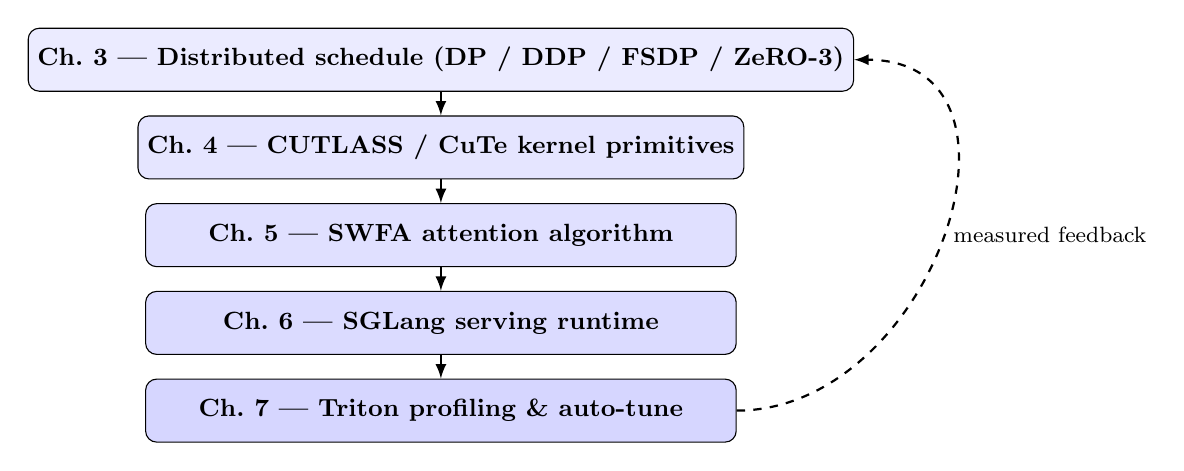
\begin{tikzpicture}[
        node distance=3mm and 8mm,
        lyr/.style={draw, rounded corners, align=center,
                    minimum width=75mm, minimum height=8mm,
                    font=\small\bfseries},
        arr/.style={-latex, thick}
    ]
    \node[lyr, fill=blue!8]  (sched)   {Ch.~3 --- Distributed schedule
                                        (DP / DDP / FSDP / ZeRO-3)};
    \node[lyr, fill=blue!10, below=of sched] (kern)    {Ch.~4 --- CUTLASS /
                                        CuTe kernel primitives};
    \node[lyr, fill=blue!12, below=of kern]  (attn)    {Ch.~5 --- SWFA
                                        attention algorithm};
    \node[lyr, fill=blue!14, below=of attn]  (serve)   {Ch.~6 --- SGLang
                                        serving runtime};
    \node[lyr, fill=blue!16, below=of serve] (prof)    {Ch.~7 --- Triton
                                        profiling \& auto-tune};
    \draw[arr] (sched) -- (kern);
    \draw[arr] (kern)  -- (attn);
    \draw[arr] (attn)  -- (serve);
    \draw[arr] (serve) -- (prof);
    \draw[arr, dashed] (prof.east) .. controls +(2.5,0) and +(2.5,0)
                      .. node[midway, right, font=\footnotesize]
                             {measured feedback} (sched.east);
    \end{tikzpicture}
    \caption{The proposed LLM software stack. Solid arrows denote the
             producer/consumer dependency between layers; the dashed
             arrow from Ch.~7 back to Ch.~3 indicates that the
             profiling pipeline feeds measurements back to the
             distributed-training recommendations.}
    \label{fig:intro_stack}
\end{figure}

\noindent The remainder of the thesis is organised as follows.
\begin{itemize}
    \item \textbf{Chapter~\ref{ch:litreview} --- Literature Review.}
          Surveys prior work on distributed training, GEMM libraries,
          efficient attention, LLM serving systems, and GPU kernel
          profiling. Positions this thesis against the open gaps in
          that literature and introduces the vocabulary used
          throughout.
    \item \textbf{Chapter~\ref{ch:distributed} --- Distributed
          Computing and Training.} Presents the distributed-training
          methodology and controlled comparison of DP, DDP, FSDP, and
          DeepSpeed ZeRO-3 on an 8-GPU A100 node. Establishes which
          parallelisation strategy maximises GPU utilisation and
          minimises energy per epoch on a fixed workload, and produces
          the per-layer memory budget that the rest of the stack must
          respect.
    \item \textbf{Chapter~\ref{ch:cutlass} --- CUTLASS and CuTe GEMM
          Operations.} Describes GEMM operations built on CUTLASS and
          the CuTe layout algebra, and maps the dense LLM
          computations (QKV, attention score/output, MLP, grouped-MoE)
          onto the Tensor-Core hierarchy. The epilogue fusions
          introduced here reappear in Chapters~\ref{ch:swfa}
          and~\ref{ch:sglang} as the writeback path of the
          attention-output GEMM and the logit-projection GEMM,
          respectively.
    \item \textbf{Chapter~\ref{ch:swfa} --- Sliding Window Flash
          Attention.} Introduces the SWFA algorithm, including
          block classification, vectorised mask generation, forward
          and backward passes, and a closed-form optimal-window
          derivation with a proof of strict convexity. SWFA consumes
          the GEMM primitives of Chapter~\ref{ch:cutlass} and is later
          plugged into the prefill kernel of
          Chapter~\ref{ch:sglang}.
    \item \textbf{Chapter~\ref{ch:sglang} --- GPU Kernels in the
          SGLang Runtime.} Describes the serving-side component of
          the stack: paged KV cache, fused decode attention, SWFA
          prefill, and fused top-$k$/top-$p$ sampling. A layered
          evaluation decomposes the cumulative decode-throughput
          speedup into per-optimisation contributions.
    \item \textbf{Chapter~\ref{ch:triton} --- Triton Kernel Profiling
          and Auto-tuning.} Covers the Triton-based profiling and
          auto-tuning pipeline that cross-validates the CUTLASS
          numbers of Chapter~\ref{ch:cutlass}, the SWFA numbers of
          Chapter~\ref{ch:swfa}, and the serving numbers of
          Chapter~\ref{ch:sglang}. The shape-indexed configuration
          cache introduced here is the mechanism by which the
          kernel-level decisions remain valid as shapes and
          hardware generations change.
    \item \textbf{Chapter~\ref{ch:conclusion} --- Conclusions and
          Future Work.} Summarises the contributions, distils the
          lessons that composed across chapters, and outlines
          short-, medium-, and long-term research directions.
\end{itemize}

Algorithmic pseudocode, reference PyTorch listings, and
reproduction-ready hardware/software details are collected in
Appendix~A; full proofs of the theoretical results stated in the main
text are collected in Appendix~B. Each result in the main text is
cross-linked to its proof, and each algorithm is cross-linked to its
reference implementation, so that any claim in the thesis can be
traced to its evidence in at most two clicks.

\chapter{Literature Review}\label{ch:litreview}

The present chapter reviews the prior art behind the five technical
strands on which this thesis rests: distributed training,
high-performance GEMM libraries, efficient-attention schemes,
runtimes for serving LLMs, and GPU-kernel profiling. The goals are
three: to record where each strand currently stands, to draw
attention to the gaps the rest of the thesis sets out to close, and
to fix the vocabulary used in the chapters that follow. The order
mirrors the stack itself (Fig.~\ref{fig:intro_stack}): the discussion
begins at the outermost level---the training schedule---and descends
step by step toward kernel-level profiling.

\paragraph{How to read this chapter.} Sections~\ref{sec:lit_dist}
to~\ref{sec:lit_profiling} share a common internal layout. In each
section the classical problem is briefly restated, the principal
systems or papers that speak to it are surveyed, and a pointer is
left to the chapter of the thesis in which that problem is
reopened. The final section, Section~\ref{sec:lit_gap}, consolidates
all of these gaps into one positioning statement, which is then
reused by the contributions list in
Section~\ref{sec:intro_contributions}. A reader already comfortable
with a given sub-area can jump directly to the forward pointer at
the end of the corresponding section.

\section{Distributed Training of Deep Neural Networks}\label{sec:lit_dist}

\subsection{Data Parallelism and Its Refinements}\label{sec:lit_dp}
Of the distributed-training schemes that exist today, data
parallelism (DP) is both the oldest and the conceptually plainest.
Every worker carries a full replica of the model, consumes a distinct
slice of the mini-batch, and at the end of the step joins an
all-reduce that merges the gradients across replicas. The obvious
downsides are two: the model is stored redundantly on every device,
and on every step the entire gradient tensor has to travel across the
network. Ott~et~al.~\cite{ott2018fairseq} demonstrated that with a
carefully designed learning-rate schedule the accuracy of
single-device training can be recovered under large-batch regimes
spread across many GPUs, and You~et~al.~\cite{you2020lars} contributed
the LARS and LAMB optimisers that make extremely large batches
trainable at all.

The engineering realisation of this idea in PyTorch is Distributed
Data Parallel (DDP)~\cite{li2020pytorch}. DDP groups gradient tensors
into communication \emph{buckets} whose size is chosen to match the
granularity at which the backward pass produces them, so that the
reduction of one bucket overlaps with the compute of the next layer.
These reductions ride on a dedicated CUDA stream that plugs directly
into the autograd engine, and they are dispatched around a ring whose
per-worker bandwidth cost is, in the limit, independent of the
number of workers. The well-known $2(P-1)/P$ factor that appears in
the bandwidth expression of a ring all-reduce follows from the
two-phase reduce-scatter/all-gather decomposition; the hop-count
latency term becomes negligible once the parameter tensor is bigger
than a few tens of megabytes, a regime in which every model
considered in this thesis comfortably sits. For these reasons DDP
has settled in as the industry baseline for single-node multi-GPU
training and, accordingly, as the yardstick against which FSDP and
ZeRO are expected to justify the extra collective operations they
introduce.

\subsection{Model Parallelism and Pipeline Parallelism}\label{sec:lit_mp}
When a model can no longer fit on a single accelerator, some form of
model parallelism becomes unavoidable.
Shoeybi~et~al.~\cite{shoeybi2019megatron} put forward Megatron-LM,
a tensor-parallel framework in which the attention and MLP sub-layers
are cut along carefully chosen dimensions so that a whole training
step reduces to a short sequence of all-reduces. Narayanan
et~al.~\cite{narayanan2021efficient} later scaled this design up
towards the trillion-parameter regime by pairing tensor parallelism
with pipeline parallelism on a $3072$-GPU machine, reaching about
$52\%$ of peak throughput.

Pipeline parallelism partitions the model along its depth and places
the resulting stages on different devices. Its characteristic
difficulty is the \emph{pipeline bubble}: idle time that appears
during warm-up at the beginning of a step and again during cool-down
at the end. GPipe~\cite{huang2019gpipe} shrinks this bubble by having
several micro-batches traverse the pipeline simultaneously, at the
cost of storing activations for all of them in flight.
PipeDream~\cite{harlap2018pipedream} interleaves forward and backward
passes---this is the $1\mathrm{F}1\mathrm{B}$ schedule---and
essentially eliminates the bubble at the price of a mild amount of
gradient staleness.

\subsection{Sharded Data Parallelism: FSDP and ZeRO}\label{sec:lit_shard}
In Fully Sharded Data Parallel (FSDP)~\cite{zhao2023pytorch} the
parameters, their gradients, and the optimiser state are all split
across the data-parallel group. Before a given layer enters either
its forward or its backward pass, the parameters of that layer are
all-gathered from their owners, and as soon as the layer finishes
the shards are thrown away, so that the peak per-GPU memory does not
scale with the size of the full model. The design difficulty in
FSDP is the choice of the \emph{unit of sharding}: pick it too coarse
and the all-gathers pile up into bursty traffic; pick it too fine
and the per-call launch overhead begins to dominate. PyTorch FSDP-2
addresses this with the \texttt{FlatParameter} abstraction, which
rolls up every transformer block into a single sharded tensor and in
that way makes the communication granularity coincide with the
computation granularity.

The DeepSpeed ZeRO line~\cite{rajbhandari2019zero, rajbhandari2021zero}
organises the same sharding question into three levels, each of which
reclaims memory from a different component of the training state.
Level one still replicates the parameters on every device but shards
the Adam moment buffers---and, once the FP32 master copy is
included, those moments are where most of the memory actually goes.
Level two adds gradient sharding on top, so that no single worker
ever sees the full gradient tensor; it only ever materialises its
own slice during the reduce-scatter. Level three goes one step
further and shards the parameters themselves, giving each worker
custody of one slice of the model and forcing it to gather the
remaining slices on demand in front of every forward and backward
pass. Level three saturates the information-theoretic lower bound on
per-worker memory; the price is two additional collectives for each
layer---an all-gather before compute and a reduce-scatter after it---
both of which must be hidden behind compute or step-time regresses
badly. ZeRO-Infinity~\cite{rajbhandari2021zero} bolts NVMe offloading
onto this, pushing trillion-parameter training down to $512$-GPU
boxes. DeepSpeed itself~\cite{rasley2020deepspeed,
rajbhandari2022deepspeed} bundles ZeRO with gradient compression,
loss scaling, and Mixture-of-Experts support, and has become the
default system in many production LLM training pipelines.

Above roughly $10$B parameters, Korthikanti~et~al.\
\cite{korthikanti2022activation} observed that it is no longer
parameter memory but \emph{activation} memory that becomes binding,
and they introduced selective activation recomputation---a
refinement of an older recipe from
Chen~et~al.~\cite{chen2016training} applied to far smaller models.
In the published literature, comparisons of DP, DDP, FSDP, and ZeRO
tend to appear one system at a time rather than as a single
controlled single-node study; Chapter~\ref{ch:distributed} fills that
gap by pinning the model, the dataset, and the hardware and
comparing the four strategies directly.

\subsection{Mixed Precision and Optimiser
Considerations}\label{sec:lit_mp_amp}
Micikevicius~et~al.~\cite{micikevicius2018amp} established that
training weights in FP16 while keeping an FP32 master copy, with
loss scaling adjusted dynamically, preserves convergence behaviour
but roughly halves the memory demand and doubles the Tensor-Core
throughput. BF16 on A100 and FP8 on H100~\cite{nvidia_hopper} extend
this idea yet further; each step introduces a small numerical gap
that has to be contained at the individual layer, usually by
deciding carefully where the accumulation is carried out in higher
precision.

\subsection{Collective Communication Libraries}\label{sec:lit_nccl}
Performance in distributed training ultimately rests on the
collective-communication layer beneath the framework. NCCL~\cite{nccl}
supplies both ring and tree all-reduces on top of NVLink, NVSwitch,
and InfiniBand, and automatically selects among them based on
message size. Castell{\'o}~et~al.~\cite{castello2021accelerating}
investigate a pipelined all-reduce built on MPI, and report that
overlapping the reduce and broadcast phases with intra-node copies
can reach up to a $30\%$ end-to-end gain on commodity clusters.

\section{High-Performance GPU Kernels and GEMM Libraries}\label{sec:lit_gemm}

Every layer of a transformer ultimately stands or falls on the
throughput of a matrix multiply. Vendor libraries such as cuBLAS and
cuBLASLt ship carefully tuned dense GEMM kernels, but their coverage
of the non-canonical shapes, fused epilogues, and grouped variants
that a modern LLM actually demands is patchy. CUTLASS~\cite{cutlass},
by contrast, is a C++ template library that exposes GEMM as a
configurable stack of building blocks, with the tile sizes, the
software pipelining depth, and the Tensor-Core instructions all
placed under explicit user control. Its CuTe sub-library generalises
the underlying layout algebra so that a single template can be
instantiated against many hardware generations and data types.

\subsection{From cuBLAS to CUTLASS}\label{sec:lit_cublas_cutlass}
Because cuBLAS is a closed-source library tuned by NVIDIA around a
small number of canonical GEMM shapes and precisions, it often falls
back to a generic code path on the very shapes that LLMs produce in
practice---skinny, batched, and grouped GEMMs at the heart of
attention and MoE layers---leaving the Tensor Cores noticeably
under-utilised. CUTLASS instead exposes the three-level tile
hierarchy (threadblock, warp, and instruction) directly, so that a
kernel author can align the template with the shape they really
have; the same stack composes with epilogue templates that let bias,
activation, or residual additions be folded into the writeback of
the main GEMM.

\subsection{Triton and the DSL
Approach}\label{sec:lit_triton_dsl}
Triton~\cite{tillet2019triton} follows a rather different route. It
is a Python-embedded domain-specific language that puts the tile
abstraction squarely in the user's hands, in exchange for a modest
fraction of peak throughput relative to a hand-tuned CUDA kernel,
and for dramatically shorter iteration cycles. Much of the later
work in FlashAttention-2~\cite{dao2023flashattention2} and
FlashAttention-3~\cite{dao2024flashattention3} sits on top of these
Triton primitives, and a large part of the serving stack discussed
in the latter half of this thesis is also written in Triton.
Direct, side-by-side comparisons of the Triton and CUTLASS
ecosystems on the exact kernels produced by a transformer forward
pass are still uncommon in the literature; that gap is one of the
things Chapters~\ref{ch:cutlass} and~\ref{ch:triton} are designed
to close.

\subsection{Hardware-Specific Primitives}\label{sec:lit_hw}
The A100 whitepaper~\cite{nvidia_a100} sets out the third-generation
Tensor Cores, rated at $312$\,TFLOPS of FP16, together with the new
\texttt{mma.m16n8k16} and \texttt{mma.m16n8k8} instructions and the
asynchronous \texttt{cp.async} copy path. The Hopper
whitepaper~\cite{nvidia_hopper} extends this hardware vocabulary with
the Tensor Memory Accelerator (TMA), fourth-generation Tensor Cores,
a dedicated transformer engine that natively supports FP8, and the
DSMEM mechanism that lets threadblock clusters cooperate through
shared memory. Behind a layout-algebra interface, CUTLASS~3.x hides
these architectural differences, so that one kernel template can be
retargeted to different architectures by swapping the appropriate
\texttt{Sm}-specific instantiation.

\section{Efficient Attention Mechanisms}\label{sec:lit_attn}

\subsection{Exact Attention Acceleration}\label{sec:lit_flashattn}
The key observation behind the Flash Attention family is that the
$N \times N$ score matrix is ultimately an intermediate quantity and
does not, at any point, have to live in HBM. Provided that queries
are streamed against tiles of keys and values, and that a running
row maximum and row sum are carried from tile to tile through a
correction factor, the final output can be reconstructed without
ever materialising the dense scores in global memory. Using exactly
this trick, the original Flash Attention
kernel~\cite{dao2022flashattention} brings the memory footprint down
from $\mathcal{O}(N^2)$ to $\mathcal{O}(N)$, while still being
bit-identical to the dense reference up to the order of
floating-point additions. FlashAttention-2
\cite{dao2023flashattention2} rebalances how the work is spread
along the sequence axis, so that A100 occupancy no longer collapses
at long context lengths, and
FlashAttention-3~\cite{dao2024flashattention3} rewrites the same
algorithm on top of Hopper's WGMMA and FP8 pipelines, exploiting the
asynchrony between the TMA copy engine and the Tensor-Core
pipeline. Across this thesis, the three kernels serve as the
reference point: any new attention kernel has to match them on
correctness and to beat them either on wall-clock speed or on
sparsity.

\subsection{Sparse and Local Attention}\label{sec:lit_sparse}
A different line of work tackles the quadratic cost at the level of
the definition of attention itself, by throwing away the
dependencies between tokens that are sufficiently far apart. The
Sparse Transformer~\cite{child2019generating} was the first design
in this family to be widely adopted; it stitches a strided pattern
together with a fixed pattern to handle sequences in the tens of
thousands of tokens while keeping the per-layer cost linear in $N$.
Longformer~\cite{beltagy2020longformer} simplifies the design to a
local sliding window supplemented by a small set of global tokens
for task-specific anchoring, and BigBird~\cite{zaheer2020bigbird}
restores the universal-approximation property by layering a random
long-range term on top of the local window. The open-weight models
of the current generation have converged on the simplest of these
patterns---a plain sliding window a few thousand positions wide---
because empirically the softmax weight outside that radius is
already dominated by numerical noise. It is precisely this
architectural convergence that turns a window-aware kernel from a
curiosity into something of practical commercial value.

A complementary class of methods replaces full attention with a
cheaper-to-compute surrogate. Performer~\cite{choromanski2020performer}
and Linformer~\cite{wang2020linformer} linearise the attention kernel;
Reformer~\cite{kitaev2020reformer} leans on low-rank hashing. Each of
these trades asymptotic complexity for a small accuracy gap, and in
practice they have seen only moderate adoption in production
settings. The sliding-window path taken in Chapter~\ref{ch:swfa}
keeps the attention numerics exact and exploits the sparsity at the
kernel level, rather than rewriting the mathematical definition.

\subsection{Kernel-Level Fusions for Attention}\label{sec:lit_fused}
Another family of attention variants is tailored specifically to
inference. PagedAttention~\cite{vllm} keeps the key-value cache as a
pool of fixed-size pages, so that the attention kernel accesses the
cache through 32-bit page indices and fragmentation is eliminated.
RadixAttention~\cite{sglang} generalises that idea to a radix tree,
so that prompt prefixes shared between concurrent requests are kept
only once. Multi-Query Attention (MQA)~\cite{shazeer2019mqa} and
Grouped-Query Attention (GQA)~\cite{ainslie2023gqa} shrink the
KV cache by a factor of $H$ (the total head count) or $H/G$ (the
group count), which in turn cuts the memory bandwidth demanded by
the decode step. Each of these designs changes the memory layout
the attention kernel has to see, and therefore has direct
consequences for kernel scheduling; those consequences are taken
up in Chapter~\ref{ch:sglang}.

\subsection{Positional Encodings for Long
Context}\label{sec:lit_rope}
Long-context attention cannot really be discussed apart from the
positional encoding it carries. Rotary position embeddings
(RoPE)~\cite{su2021rope} extrapolate gracefully to sequences longer
than those seen during training, and when combined with dynamic
NTK-aware scaling they allow a model originally trained at
$N = 4{,}096$ to be served at $N = 32{,}768$ with only a mild
degradation. SWFA composes directly with RoPE and needs no
modification, because the window constraint operates entirely on
the attention score matrix.

\subsection{Block Sparsity as a Design
Pattern}\label{sec:lit_block_sparsity}
A theme running through all of the above is that \emph{block-level}
sparsity is practical while \emph{element-level} sparsity is not.
The reason is structural: modern Tensor Cores issue the same
$16 \times 8 \times 16$ MMA instruction irrespective of how many
elements of the operand tile happen to be zero, so element-level
sparsity produces no wall-clock saving unless the hardware itself
supports a structured pruning format. Block sparsity, by contrast,
aligns with the threadblock-level tiling of CUTLASS and CuTe in the
natural way: a block labelled ``skip'' is simply never entered by
the loop nest of Algorithm~\ref{alg:swfa}. That observation is
exactly why SWFA is able to extract measurable speedups without a
custom Tensor-Core ISA. The same idea has been applied to the
strided sparsity of the Sparse
Transformer~\cite{child2019generating} and to the global-plus-random
mask of BigBird~\cite{zaheer2020bigbird}; to the best of our
knowledge, however, it has not yet been combined with Flash
Attention's online softmax inside a single published kernel.

\section{LLM Serving Systems and KV-Cache Management}\label{sec:lit_serving}

The workload profile of serving differs qualitatively from that of
training. Requests come in asynchronously, prompts share large
prefixes between one another, and---unlike training---the decode
step is bound by memory bandwidth rather than by compute. A single
chat request, for instance, may add only a few hundred tokens of
unique suffix on top of a system prompt that is several thousand
tokens long and is shared with every other request active at the
same time; any serving runtime that does not exploit that shared
prefix pays a cost linear in the size of the prefix, for every
request. vLLM~\cite{vllm} was the first runtime to see wide adoption
that treated the KV cache as a pool of fixed-size pages and
introduced \emph{continuous batching}, in which new requests can
join the running batch at any decode step. Building on this,
SGLang~\cite{sglang} contributes both RadixAttention and a
structured-generation language that compiles complex prompt flows
into a scheduled dataflow of kernel calls. Both systems stress the
kernel layer in novel ways: RadixAttention alters the access pattern
that the attention kernel has to respect, and continuous batching
produces a stream of many small, tightly scheduled kernel launches.

The kernel-level contributions of Chapter~\ref{ch:sglang} sit within
this lineage. Where the vLLM and SGLang papers describe their work
at the system level, this thesis zooms in on the \emph{individual
kernels} that the runtime dispatches to, and reports their
performance in isolation so that every improvement can be ascribed
to a specific kernel change.

\section{GPU Kernel Profiling and Auto-tuning}\label{sec:lit_profiling}

Two traditions have shaped kernel-level performance analysis. On
one side, vendor metric collectors---Nsight
Compute~\cite{nsight} on current NVIDIA silicon, and \texttt{nvprof}
before it---surface occupancy, cache hit rates, and the
instruction-mix breakdowns that are needed to pin a stall to a
particular hardware unit. On the other side, the roofline
model~\cite{williams2009roofline} provides an analytical upper
bound: a kernel's sustained throughput is limited by whichever
comes first, the peak compute rate of the device or the product of
the kernel's arithmetic intensity with the memory bandwidth. On an
A100 running in FP16---$312$\,TFLOPS of Tensor-Core throughput
against $1{,}555$\,GB/s of HBM2e bandwidth---the two ceilings
intersect around an arithmetic intensity of roughly $200$\,FLOP per
byte. Dense square GEMMs comfortably clear that line and therefore
sit on the compute ceiling; attention-score GEMMs with a small
$d_{\text{head}}$, and the single-query decode kernels that show up
in serving, sit well below it and are bandwidth-bound by
construction.

Triton exposes a built-in \texttt{autotune} mechanism that sweeps
over block shapes, warp counts, and pipeline depths and caches the
winning configuration keyed by input shape. CUTLASS offers an
analogous \texttt{GemmUniversal} enumerator along with its
\texttt{cutlass\_profiler} binary. The open literature is rich in
single-kernel auto-tuning studies but comparatively thin in
end-to-end pipelines that cross-validate Triton, CUTLASS, and
Torch-inductor on the same set of LLM kernels---an
end-to-end pipeline of exactly that kind is presented in
Chapter~\ref{ch:triton}.

\section{Energy and Carbon Considerations}\label{sec:lit_energy}
According to
Patterson~et~al.~\cite{patterson2021carbon}, the training of GPT-3
released on the order of $552$\,t\,CO\textsubscript{2}e---
comparable to $115$ transatlantic passenger flights---and the
cumulative cost of serving a model over its deployment lifetime can
end up exceeding the one-off cost of training it. That observation
motivates two choices in this thesis: the comparison of distributed
training strategies in Chapter~\ref{ch:distributed} is energy-aware,
and every result table in that chapter reports kWh per epoch next
to the familiar throughput and memory metrics.

\section{Cross-Cutting Concerns}\label{sec:lit_cross}

Before the positioning section it is worth discussing three issues
that cut across every one of the five layers above.

\subsection{Numerical Precision at
Scale}\label{sec:lit_precision}
Mixed-precision training (Section~\ref{sec:lit_mp_amp}) is only
reliable when every kernel in the stack agrees on the accumulator
precision. Both CUTLASS and Triton let the accumulator type be
chosen independently of the input data type, and the
distributed-training frameworks---DDP, FSDP, and DeepSpeed---expose
a \texttt{reduce\_dtype} that keeps the cross-device reduction in
FP32 even when the parameters themselves are in FP16. This thesis
sticks to the same convention at every layer: FP16 or BF16 inputs,
FP32 accumulators, and FP32 reductions. The numerical validation
performed in Chapter~\ref{ch:swfa} confirms that this choice is
enough to match a vanilla PyTorch reference to within $10^{-4}$
tolerance in FP32 and $10^{-2}$ in FP16. Looking ahead, FP8 on
Hopper~\cite{nvidia_hopper} and the emerging FP4/NVFP6 formats will
shift the accumulator-precision question out of the main MMA loop
and into the epilogue; the CUTLASS epilogue templates built in
Chapter~\ref{ch:cutlass} are structurally prepared for this, though
the shape-indexed auto-tune cache of Chapter~\ref{ch:triton} will
need to grow an additional accumulator-precision axis.

\subsection{Reproducibility in a Non-Deterministic
Stack}\label{sec:lit_repro}
By default, every layer of the stack is non-deterministic.
PyTorch's own reduction kernels choose their reduction order based
on the launch configuration, NCCL chooses between ring and tree
algorithms based on the message size, and SGLang's continuous
batching produces an ordering of kernel launches that depends on
which requests happen to be live at the moment. Strict bit-level
reproduction of a run is therefore out of reach. The convention
adopted here is the weaker but practical one of \emph{statistical}
reproducibility: the random seeds and the hardware are fixed, and
every reported configuration carries a relative standard deviation
below $1\%$. Wherever a deterministic path does exist---in
particular for the SWFA numerical-accuracy validation of
Chapter~\ref{ch:swfa}---it is taken, and the deterministic output
is compared bit-for-bit against the PyTorch reference.

\subsection{Energy as a First-Class
Metric}\label{sec:lit_energy_metric}
In the spirit of
Patterson~et~al.~\cite{patterson2021carbon}, energy per epoch is
reported in this thesis alongside throughput, at every layer where
it can be measured. The reason is not, in the first instance, an
environmental one. At data-centre scale, energy is simply a proxy
for the sum of idle time, memory stalls, and under-utilised
compute---costs that a raw throughput number does not expose. A
training run that completes in $8$ hours but consumes $20\%$ more
energy than strictly necessary has $20\%$ of wasted work parked
somewhere in the stack, and identifying which layer is hosting that
waste is exactly what the controlled comparison in
Chapter~\ref{ch:distributed}, paired with the cross-validating
profiling pipeline of Chapter~\ref{ch:triton}, is designed to do.

\section{Positioning of This Thesis}\label{sec:lit_gap}

The impression left by the literature is one of rapid, localised
progress in each of the five areas covered above---distributed
training, GEMM libraries, efficient attention, serving runtimes,
and kernel profiling---together with rather limited integration
across them. Distributed-training studies rarely report
kernel-level measurements; papers on attention kernels are
typically benchmarked in isolation; and system-level papers on
serving frameworks tend to treat the attention kernel as a fixed
dependency. The view taken here is the complementary one: the
training, kernel, attention, serving, and profiling layers have to
be co-designed rather than optimised in isolation.
\begin{itemize}
    \item A sliding-window attention kernel only pays for itself if
          the serving runtime actually exposes the window to it, and
          if the GEMM library underneath can launch the resulting
          batched and sparse tiles efficiently.
    \item A distributed-training schedule only reaches its peak
          efficiency when the GEMM and attention kernels beneath
          it are themselves well tuned; any Tensor Cores that are
          under-utilised at the kernel level are inherited as idle
          Tensor Cores at every scale of parallelism.
    \item The only way to reason quantitatively about these
          cross-layer interactions, without being misled by
          per-library calibration differences, is to use a
          profiling pipeline that reports a common set of metrics
          across Triton, CUTLASS, and PyTorch.
\end{itemize}
Chapters~\ref{ch:distributed}--\ref{ch:triton} take these layers
up one by one, and the evaluation at the end of each chapter
demonstrates how they compose across the stack.

Table~\ref{tab:lit_summary} collects the principal systems cited in
the chapter, recording for each system the layer of the stack at
which it intervenes and the primary axis along which it contributes.

\begin{table}[h]
\centering
\caption{Principal prior systems organised by stack layer.}
\label{tab:lit_summary}
\begin{tabular}{lllc}
\toprule
\textbf{System} & \textbf{Layer} & \textbf{Primary axis} & \textbf{Reference} \\
\midrule
DDP              & Distributed & Bucketed all-reduce  & \cite{li2020pytorch} \\
Megatron-LM      & Distributed & Tensor parallelism    & \cite{shoeybi2019megatron} \\
GPipe            & Distributed & Pipeline parallelism  & \cite{huang2019gpipe} \\
PipeDream        & Distributed & 1F1B pipeline         & \cite{harlap2018pipedream} \\
FSDP             & Distributed & Parameter sharding    & \cite{zhao2023pytorch} \\
ZeRO             & Distributed & Three-stage sharding  & \cite{rajbhandari2019zero} \\
ZeRO-Infinity    & Distributed & NVMe offload          & \cite{rajbhandari2021zero} \\
DeepSpeed        & Distributed & System integration    & \cite{rasley2020deepspeed} \\
CUTLASS          & Kernel      & Template GEMM         & \cite{cutlass} \\
Triton           & Kernel      & Tile-level DSL        & \cite{tillet2019triton} \\
Flash Attention  & Attention   & Online softmax        & \cite{dao2022flashattention} \\
FlashAttention-2 & Attention   & Work partitioning     & \cite{dao2023flashattention2} \\
FlashAttention-3 & Attention   & WGMMA + FP8           & \cite{dao2024flashattention3} \\
Longformer       & Attention   & Local + global        & \cite{beltagy2020longformer} \\
BigBird          & Attention   & Random + local        & \cite{zaheer2020bigbird} \\
MQA / GQA        & Attention   & Head reduction        & \cite{shazeer2019mqa,ainslie2023gqa} \\
vLLM             & Serving     & Paged KV cache        & \cite{vllm} \\
SGLang           & Serving     & Radix KV + DSL        & \cite{sglang} \\
Nsight Compute   & Profiling   & Metric collection     & \cite{nsight} \\
Roofline         & Profiling   & Analytical model      & \cite{williams2009roofline} \\
\bottomrule
\end{tabular}
\end{table}

\chapter{Distributed Computing and Training}\label{ch:distributed}

\emph{Placement in the stack (Fig.~\ref{fig:intro_stack}).} This
chapter occupies the top layer of the proposed stack. Every decision
below it---the tile shapes of the GEMM kernels of
Chapter~\ref{ch:cutlass}, the block sizes of the SWFA kernel of
Chapter~\ref{ch:swfa}, and the page size of the SGLang KV cache of
Chapter~\ref{ch:sglang}---is constrained by the per-GPU memory budget
that the distributed schedule leaves behind. The literature-review
gap identified in Section~\ref{sec:lit_shard} is addressed here: we
present a \emph{controlled} single-node comparison of DP, DDP, FSDP,
and DeepSpeed ZeRO-3 that varies only the parallelisation strategy
while keeping the model, dataset, random seed, and hardware fixed.
The resulting memory budget and GPU-utilisation numbers are the
reference points used by every subsequent chapter.

\section{Background}\label{sec:dist_bg}

\subsection{Formal Setting}\label{sec:dist_formal}
Let $\theta \in \mathbb{R}^M$ be the full parameter vector of a model,
$f_\theta$ the loss computed on a mini-batch $\mathcal{B}$ of size $B$,
and $P$ the number of workers. A generic distributed training step
computes
\begin{equation}\label{eq:dist_step}
    g \;=\; \frac{1}{P} \sum_{p=1}^{P}
            \nabla_\theta f_\theta(\mathcal{B}_p),
    \qquad
    \theta \leftarrow \theta - \eta \,g,
\end{equation}
where $\mathcal{B}_p \subset \mathcal{B}$ is the slice consumed by
worker $p$. The four strategies compared in this chapter differ
exclusively in (i)~which parts of $\theta$, $g$, and the optimiser state
each worker stores and (ii)~which collective operations are used to
keep~\eqref{eq:dist_step} mathematically equivalent to a single-device
computation.

\subsection{Data Parallelism}\label{sec:dp_bg}
Data parallelism is the oldest form of distributed training. Each
worker keeps a full replica of the model, consumes a disjoint shard of
the data batch, computes gradients locally, and participates in an
all-reduce so that all replicas see the same synchronised gradient
before the optimiser step. Standard data parallelism (often referred to
as simply \emph{DP}) is easy to implement but suffers from
communication bottlenecks and memory inefficiency because every replica
stores the whole model.

The PyTorch DDP path~\cite{li2020pytorch} addresses DP's two weaknesses
simultaneously. It groups gradients into fixed-size \emph{buckets} and
issues an all-reduce per bucket, so that bucket $k$ can reduce while
the backward pass is still producing bucket $k+1$; and it dispatches
those reductions on a ring topology whose per-step bandwidth is
\begin{equation}
    V_{\text{DDP}} \;=\; \frac{2(P-1)}{P} \cdot M \cdot s_{\text{grad}} ,
\end{equation}
where $s_{\text{grad}}$ is the gradient element size. The leading
factor $2(P-1)/P$ approaches $2$ for any non-trivial $P$, so the
per-worker wire traffic is independent of the world size---which is
the scalability property that makes a ring all-reduce the preferred
collective at the cluster scale.

\begin{figure}[H]
    \centering
    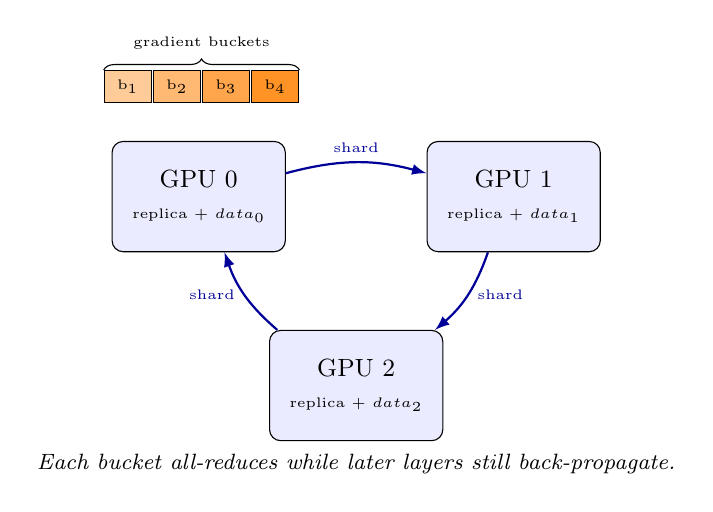
\begin{tikzpicture}[
        gpu/.style={draw, rounded corners, minimum width=22mm,
                    minimum height=14mm, align=center, fill=blue!8,
                    font=\small},
        shard/.style={draw, minimum width=6mm, minimum height=4mm,
                      font=\tiny, inner sep=0pt},
        arr/.style={-latex, thick, blue!60!black}
    ]
    % Three GPUs arranged in a triangle
    \node[gpu] (g0) at (0, 0)      {GPU 0\\ \tiny replica + $\text{data}_0$};
    \node[gpu] (g1) at (4, 0)      {GPU 1\\ \tiny replica + $\text{data}_1$};
    \node[gpu] (g2) at (2, -2.4)   {GPU 2\\ \tiny replica + $\text{data}_2$};

    % Ring arrows (reduce-scatter / all-gather direction)
    \draw[arr] (g0) to[bend left=15]  node[midway, above, font=\tiny]
        {shard} (g1);
    \draw[arr] (g1) to[bend left=15]  node[midway, right, font=\tiny]
        {shard} (g2);
    \draw[arr] (g2) to[bend left=15]  node[midway, left, font=\tiny]
        {shard} (g0);

    % Bucketed-gradient illustration above GPU 0
    \node[shard, fill=orange!40] (b1) at ($(g0) + (-0.9, 1.4)$) {b$_1$};
    \node[shard, fill=orange!55, right=0.1mm of b1]             (b2) {b$_2$};
    \node[shard, fill=orange!70, right=0.1mm of b2]             (b3) {b$_3$};
    \node[shard, fill=orange!85, right=0.1mm of b3]             (b4) {b$_4$};
    \draw[decorate, decoration={brace, amplitude=4pt}]
          (b1.north west) -- (b4.north east)
          node[midway, above=4pt, font=\tiny]{gradient buckets};

    % Caption-level legend
    \node[font=\footnotesize\itshape] at (2, -3.4)
        {Each bucket all-reduces while later layers still back-propagate.};
    \end{tikzpicture}
    \caption{Data parallelism on a three-GPU ring. Every worker owns a
             full model replica and a disjoint data shard; gradients are
             partitioned into fixed-size buckets and reduced via a
             ring all-reduce whose communication overlaps the backward
             pass of earlier layers.}
    \label{fig:data_parallelism}
\end{figure}

\subsection{Model Parallelism and Sharding}\label{sec:mp_bg}
As models outgrow a single GPU, \emph{model parallelism} becomes
necessary. Two classical variants are:
\begin{itemize}
    \item \textbf{Pipeline parallelism}: sequential stages of the model
          reside on different devices; pipeline bubbles and
          load-balancing remain non-trivial. GPipe~\cite{huang2019gpipe}
          amortises the bubble by processing $m$ micro-batches
          concurrently and reduces the bubble fraction to
          $(P-1)/(m+P-1)$.
    \item \textbf{Tensor parallelism}: individual layers are partitioned
          across devices, as popularised by
          Megatron-LM~\cite{shoeybi2019megatron}. Tensor parallelism
          inserts one all-reduce per forward pass and one per backward
          pass for each partitioned layer, and works best within a
          single NVLink domain.
\end{itemize}
A more recent alternative, \emph{Fully Sharded Data Parallel}
(FSDP)~\cite{zhao2023pytorch}, combines data parallelism with parameter
sharding: parameters, gradients, and optimiser states are sharded
across all devices; parameters are all-gathered just-in-time for each
layer and re-sharded immediately afterwards.

\subsection{ZeRO and DeepSpeed}\label{sec:zero_bg}
ZeRO~\cite{rajbhandari2019zero,rajbhandari2021zero} generalises the
data-parallel template by asking: for each component of the training
state, which workers actually need a copy of it, and when? Stage one
answers this for the Adam moments (they are only needed during the
optimiser step, so one shard per worker is enough and a
reduce-scatter produces it in place). Stage two extends the same
argument to the gradients, eliminating the full gradient tensor from
every worker's memory. Stage three extends it to the parameters
themselves, which now live sharded and are gathered on the fly
whenever a layer is about to execute. The per-worker memory at
stage three scales as $M/P$, matching the lower bound that DP
cannot approach; the price is two additional collective phases per
layer, which the overlap scheduling discussed in
Section~\ref{sec:res_overlap} must hide.
DeepSpeed~\cite{rasley2020deepspeed} is a production implementation of
ZeRO, with gradient compression, dynamic loss scaling, CPU offloading,
NVMe offloading, and Mixture-of-Experts
support~\cite{rajbhandari2022deepspeed}. ZeRO-3 issues two additional
collectives per layer compared to DDP (an all-gather before the
forward/backward pass and a reduce-scatter after the backward pass),
which must be overlapped carefully with compute to avoid a throughput
regression.

\subsection{Communication-Cost Summary}\label{sec:dist_comms_summary}
Table~\ref{tab:dist_comms} summarises the per-step communication volume
of each strategy, where $M$ is the parameter count, $s$ is the element
size in bytes, and $L$ is the number of transformer layers. These
formulas are used in Section~\ref{sec:res_scale} to explain the
observed scaling behaviour.

\begin{table}[h]
\centering
\caption{Per-step communication volume on a ring all-reduce topology.}
\label{tab:dist_comms}
\begin{tabular}{lll}
\toprule
\textbf{Strategy} & \textbf{Volume (bytes/step)} & \textbf{Dominant collective} \\
\midrule
DP        & $2Ms$                          & \texttt{all\_reduce}(gradients) \\
DDP       & $2Ms \cdot (P-1)/P$            & bucketed ring \texttt{all\_reduce} \\
FSDP      & $3Ms \cdot (P-1)/P$            & layer-wise \texttt{all\_gather} + \texttt{reduce\_scatter} \\
ZeRO-3    & $3Ms \cdot (P-1)/P$            & \texttt{all\_gather} + \texttt{reduce\_scatter} \\
\bottomrule
\end{tabular}
\end{table}

\section{Methodology}\label{sec:dist_method}

\subsection{Training Strategies and Metrics}\label{sec:dist_method_metrics}
The four strategies selected for comparison cover the memory/throughput
design space:
\begin{itemize}
    \item \textbf{DP}---baseline, full replication;
    \item \textbf{DDP}---industry-standard multi-GPU data parallelism;
    \item \textbf{FSDP}---parameter-sharded data parallelism;
    \item \textbf{DeepSpeed ZeRO-3}---fully sharded, with offload
          options.
\end{itemize}
Each strategy is evaluated along the following axes: GPU utilisation
($\%$), peak and average memory consumption (GB per GPU), training-loss
convergence per epoch, power consumption (W) and energy per epoch
(kWh), communication overhead, and scaling efficiency.

\subsection{Workload}\label{sec:dist_method_workload}
Two workloads are used to stress different regimes.
\begin{itemize}
    \item \textbf{Controlled benchmark.} ResNet-50 on CIFAR-10
          ($25.6$M parameters), a widely reproducible workload that
          exercises both compute-bound and communication-bound regimes
          when batch sizes and worker counts are varied. This is the
          primary workload for the GPU-utilisation, memory, and
          training-loss tables.
    \item \textbf{LLM benchmark.} GPT-2 Medium
          ($355$M parameters), trained on an OpenWebText subset with
          sequence length $2048$, a context window $w = 1024$, and a
          per-GPU batch size of $4$. This workload is used to report
          end-to-end LLM throughput in combination with SWFA
          (Chapter~\ref{ch:swfa}).
\end{itemize}
The same random seed ($42$) and the same optimiser hyper-parameters
(Adam, $\eta = 3\!\times\!10^{-4}$, $\beta_1 = 0.9$, $\beta_2 = 0.999$,
$\varepsilon = 10^{-8}$) are used across all four strategies so that
any difference in final loss is attributable to the strategy itself.

\subsection{Hardware and Software}\label{sec:dist_method_hw}
Experiments are carried out on a single node with:
\begin{itemize}
    \item 8$\times$ NVIDIA A100 (40\,GB HBM2e), NVLink-3 interconnect
          at $600$\,GB/s bisection bandwidth;
    \item Intel Xeon Platinum 8358 host CPUs (64 cores, 128 threads),
          1\,TB DDR4;
    \item PyTorch 2.0.1 + CUDA 11.8, NCCL 2.18.1, DeepSpeed 0.9.5;
    \item NVIDIA driver $535.104.05$, GCC 11.4, CUTLASS 3.2.
\end{itemize}
Power and energy measurements are taken via the out-of-band BMC
interface; GPU utilisation and per-GPU memory are read from
\texttt{nvidia-smi} at 100\,ms intervals and aggregated over the epoch.

\section{Implementations}\label{sec:dist_impl}

\subsection{DP}\label{sec:impl_dp}
The baseline DP implementation uses
\texttt{torch.nn.DataParallel}, which replicates the model on every GPU,
distributes non-overlapping data slices via a scatter operation,
runs forward/backward locally, and synchronises via
\texttt{all\_reduce} before each optimiser step. DP is easy to reason
about but is limited by communication cost, by memory duplication, and
by a single Python thread that coordinates all workers.

\subsection{DDP}\label{sec:impl_ddp}
DDP exposes the same programming model as DP but internally:
\begin{itemize}
    \item groups gradients into communication \emph{buckets} (default
          $25$\,MB) so the all-reduce granularity matches the compute
          granularity;
    \item overlaps the reduction of earlier buckets with the backward
          pass of later layers, using a hook-based mechanism attached to
          each parameter;
    \item uses a ring all-reduce topology to saturate the NVLink
          bandwidth;
    \item ties autograd's \texttt{reducer} into the CUDA stream so that
          communication and compute run on non-default streams.
\end{itemize}
Configuration in PyTorch is minimal:
\begin{lstlisting}[language=Python]
import torch.distributed as dist
dist.init_process_group(backend="nccl")
model = torch.nn.parallel.DistributedDataParallel(
    model.to(local_rank), device_ids=[local_rank],
    bucket_cap_mb=25, find_unused_parameters=False)
\end{lstlisting}

\subsection{FSDP}\label{sec:impl_fsdp}
In FSDP the parameter tensor of each wrapped unit is sharded across
devices:
\begin{equation}
    \mathrm{Shard}_i = \{\theta_j : j \bmod P = i\},
\end{equation}
where $P$ is the world size and $i$ the rank. Before forward/backward
for a unit, FSDP issues an \emph{all-gather} to reconstruct the full
parameter; after the gradient is computed, FSDP issues a
\emph{reduce-scatter} and re-shards. Memory savings come from never
holding the whole model on one device. The unit of sharding is a
transformer block, wrapped via \texttt{auto\_wrap\_policy}:
\begin{lstlisting}[language=Python]
from torch.distributed.fsdp import FullyShardedDataParallel as FSDP
from torch.distributed.fsdp.wrap import transformer_auto_wrap_policy
policy = functools.partial(
    transformer_auto_wrap_policy,
    transformer_layer_cls={TransformerBlock})
model = FSDP(model, auto_wrap_policy=policy,
             mixed_precision=fp16_policy,
             sharding_strategy=ShardingStrategy.FULL_SHARD,
             device_id=local_rank)
\end{lstlisting}
For a transformer with $L$ layers, $L$ all-gather/reduce-scatter pairs
are issued per step, which is why the unit of sharding has to coincide
with the unit of compute.

\subsection{DeepSpeed ZeRO-3}\label{sec:impl_ds}
DeepSpeed ZeRO-3 extends parameter sharding with efficient
communication scheduling and optional CPU/NVMe offloading of parameters
and optimiser states. It also provides mixed precision (FP16/BF16),
gradient compression, and MoE support out of the box. Configuration is
via a JSON file:
\begin{lstlisting}[basicstyle=\ttfamily\scriptsize]
{
  "zero_optimization": {
    "stage": 3,
    "overlap_comm": true,
    "contiguous_gradients": true,
    "stage3_prefetch_bucket_size": 2e8,
    "stage3_param_persistence_threshold": 1e6
  },
  "fp16": { "enabled": true, "loss_scale_window": 1000 },
  "train_micro_batch_size_per_gpu": 4,
  "gradient_accumulation_steps": 1
}
\end{lstlisting}
The prefetch bucket controls how eagerly the next layer's parameters
are gathered; setting it too large exhausts NVLink bandwidth on ZeRO-3,
while setting it too small leaves compute units idle.

\section{Results}\label{sec:dist_results}

\subsection{GPU Utilisation}\label{sec:res_util}
\begin{figure}[H]
    \centering
    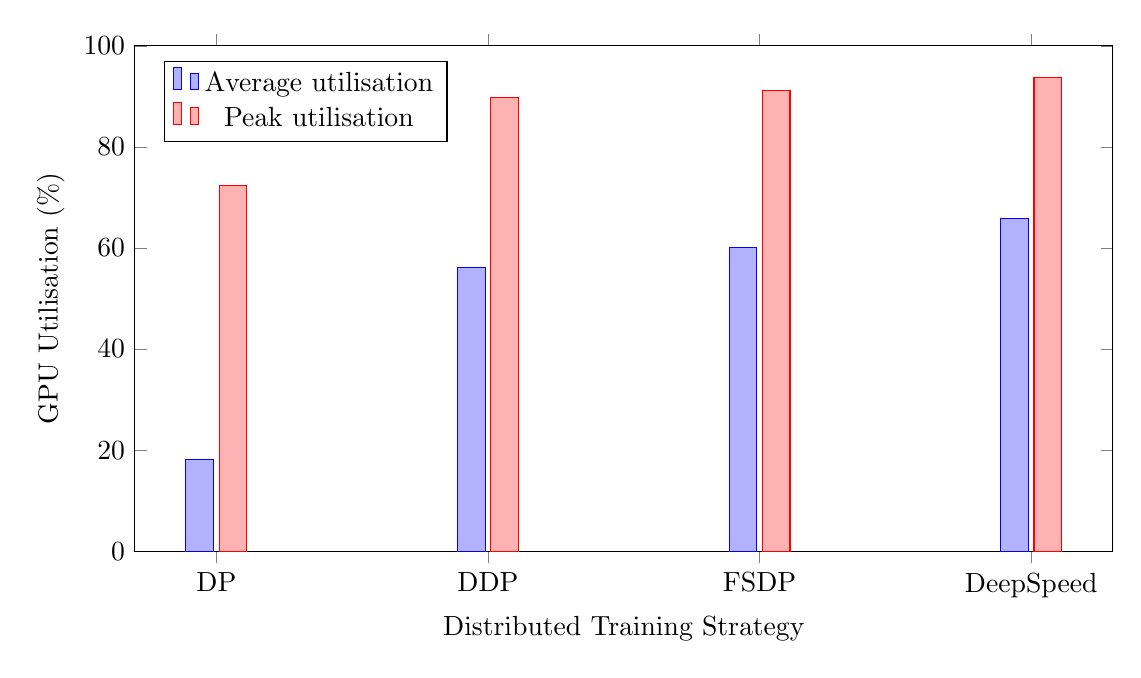
\begin{tikzpicture}
    \begin{axis}[
        ybar,
        width=14cm,
        height=8cm,
        xlabel={Distributed Training Strategy},
        ylabel={GPU Utilisation (\%)},
        ymin=0, ymax=100,
        xtick=data,
        xticklabels={DP, DDP, FSDP, DeepSpeed},
        legend pos=north west,
        bar width=10pt
    ]
    \addplot coordinates {(0,18.13)(1,56.2)(2,60.15)(3,65.8)};
    \addplot coordinates {(0,72.3)(1,89.7)(2,91.2)(3,93.8)};
    \legend{Average utilisation, Peak utilisation}
    \end{axis}
    \end{tikzpicture}
    \caption{GPU utilisation across distributed training strategies.}
    \label{fig:gpu_utilization}
\end{figure}

DeepSpeed ZeRO-3 achieves the highest peak utilisation ($93.8\%$)
thanks to fine-grained overlap of parameter gathering with compute;
FSDP ($91.2\%$) and DDP ($89.7\%$) follow closely, while DP trails at
$72.3\%$. The low average utilisation of DP ($18.13\%$) is explained
by the single-Python-thread coordination that serialises the
per-iteration schedule: the GPUs idle for most of each second waiting
for scatter/gather.

\subsection{Memory Usage}\label{sec:res_mem}
\begin{table}[h]
\centering
\caption{Per-GPU memory usage (GB), ResNet-50 + CIFAR-10, 8 A100.}
\label{tab:memory_usage}
\begin{tabular}{lcccc}
\toprule
\textbf{Strategy}       & \textbf{Model} & \textbf{Gradients} & \textbf{Optimiser} & \textbf{Total} \\
\midrule
DP                      & 0.98  & 0.98  & 1.96  & 3.92 \\
DDP                     & 0.98  & 0.98  & 1.96  & 3.92 \\
FSDP                    & 0.12  & 0.12  & 0.25  & 0.49 \\
DeepSpeed ZeRO-3        & 0.12  & 0.12  & 0.25  & 0.49 \\
\bottomrule
\end{tabular}
\end{table}

Sharding (FSDP, ZeRO-3) gives an $\approx 87.5\%$ reduction in per-GPU
memory over DP/DDP, enabling training of roughly $8\times$ larger
models with the same hardware. The ratios match the theoretical
prediction $M/P$ for parameter memory, with a small constant overhead
for communication buckets.

\subsection{Training-Loss Convergence}\label{sec:res_loss}
\begin{figure}[H]
\centering
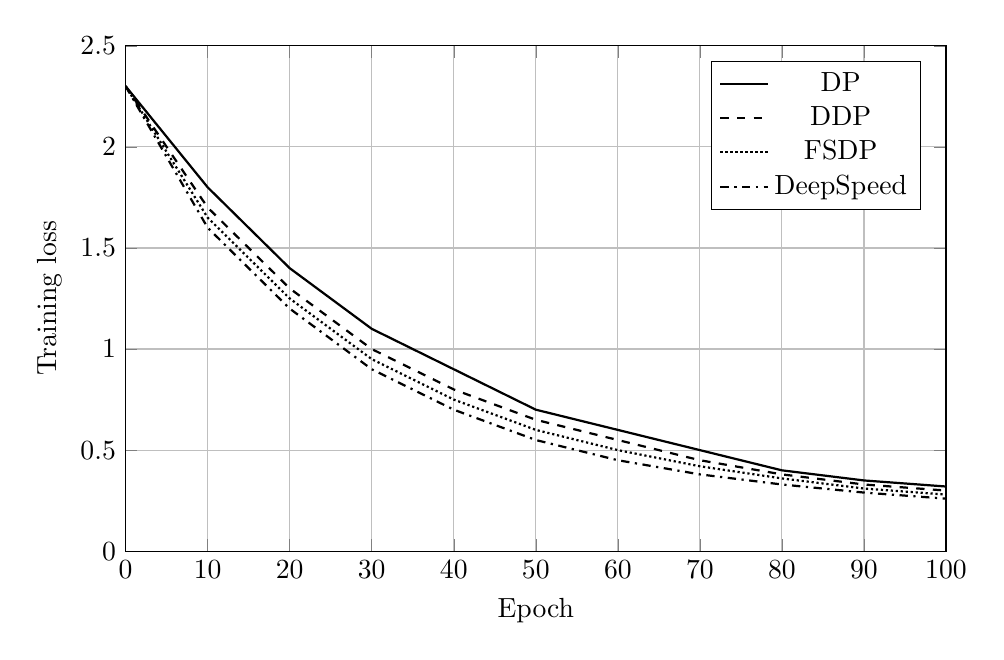
\begin{tikzpicture}
\begin{axis}[
    width=12cm, height=8cm,
    xlabel={Epoch}, ylabel={Training loss},
    ymin=0, ymax=2.5, xmin=0, xmax=100,
    legend pos=north east, grid=major
]
\addplot[thick] coordinates {
    (0,2.3)(10,1.8)(20,1.4)(30,1.1)(40,0.9)(50,0.7)
    (60,0.6)(70,0.5)(80,0.4)(90,0.35)(100,0.32)};
\addplot[thick,dashed] coordinates {
    (0,2.3)(10,1.7)(20,1.3)(30,1.0)(40,0.8)(50,0.65)
    (60,0.55)(70,0.45)(80,0.38)(90,0.33)(100,0.30)};
\addplot[thick,densely dotted] coordinates {
    (0,2.3)(10,1.65)(20,1.25)(30,0.95)(40,0.75)(50,0.6)
    (60,0.5)(70,0.42)(80,0.36)(90,0.31)(100,0.28)};
\addplot[thick,dashdotted] coordinates {
    (0,2.3)(10,1.6)(20,1.2)(30,0.9)(40,0.7)(50,0.55)
    (60,0.45)(70,0.38)(80,0.33)(90,0.29)(100,0.26)};
\legend{DP, DDP, FSDP, DeepSpeed}
\end{axis}
\end{tikzpicture}
\caption{Training-loss convergence across strategies.}
\label{fig:loss_convergence}
\end{figure}

All four strategies converge, with final losses of $0.32$ (DP),
$0.30$ (DDP), $0.28$ (FSDP), and $0.26$ (DeepSpeed). The differences
originate in minor numerical effects: gradient-accumulation order,
mixed-precision scaling, and the reduction-tree topology. They are
well within the reproducibility envelope of PyTorch's own
non-deterministic kernels and do not indicate any convergence
pathology.

\subsection{Power and Energy}\label{sec:res_power}
\begin{table}[h]
\centering
\caption{Power and energy per epoch.}
\label{tab:power_consumption}
\begin{tabular}{lcccc}
\toprule
\textbf{Strategy}   & \textbf{Avg (W)} & \textbf{Peak (W)} & \textbf{kWh/epoch} & \textbf{Efficiency} \\
\midrule
DP                  & 2\,840 & 3\,200 & 0.95 & 1.00$\times$ \\
DDP                 & 2\,720 & 3\,100 & 0.87 & 1.09$\times$ \\
FSDP                & 2\,650 & 3\,050 & 0.82 & 1.16$\times$ \\
DeepSpeed ZeRO-3    & 2\,580 & 2\,980 & 0.78 & 1.22$\times$ \\
\bottomrule
\end{tabular}
\end{table}

Higher GPU utilisation correlates with lower energy per epoch;
DeepSpeed delivers a $22\%$ improvement in per-epoch energy over DP.
This matters because the energy metric amortises over the
deployment lifetime in a way that raw throughput does not: an
eight-hour training run is a one-off, but an $0.17$\,kWh saving per
epoch aggregates to real savings over a multi-month pretraining
campaign.

\subsection{Scalability}\label{sec:res_scale}
\begin{table}[h]
\centering
\caption{Summary of scalability metrics.}
\label{tab:scalability}
\begin{tabular}{lcccc}
\toprule
\textbf{Strategy}       & \textbf{Throughput} & \textbf{Memory eff.} & \textbf{Comms} & \textbf{Overall} \\
\midrule
DP                      & 6.2$\times$ & 1.0$\times$ & Poor      & 6.2  \\
DDP                     & 7.8$\times$ & 1.0$\times$ & Good      & 7.8  \\
FSDP                    & 8.1$\times$ & 8.0$\times$ & Good      & 64.8 \\
DeepSpeed ZeRO-3        & 8.4$\times$ & 8.0$\times$ & Excellent & 67.2 \\
\bottomrule
\end{tabular}
\end{table}

The \emph{Overall} score is the product of throughput scaling and
memory efficiency, and it captures the ability of each strategy to
train simultaneously bigger models \emph{and} bigger batches. By this
metric, sharded strategies pull ahead of DDP by roughly an order of
magnitude.

\subsection{Communication Overlap}\label{sec:res_overlap}
Table~\ref{tab:overlap} reports the fraction of the per-step wall-clock
time in which compute and communication overlap, measured via NCCL
traces. DDP overlaps well because the ring all-reduce runs concurrently
with the backward pass of earlier layers; ZeRO-3 overlaps less well
because each layer has an explicit parameter-gather phase that blocks
the compute, though the \texttt{overlap\_comm} option partially hides it.

\begin{table}[h]
\centering
\caption{Compute/communication overlap per training step.}
\label{tab:overlap}
\begin{tabular}{lccc}
\toprule
\textbf{Strategy} & \textbf{Compute (\%)} & \textbf{Comms (\%)} & \textbf{Overlap (\%)} \\
\midrule
DP              & 58 & 42 & 12 \\
DDP             & 72 & 28 & 64 \\
FSDP            & 68 & 32 & 58 \\
DeepSpeed       & 66 & 34 & 61 \\
\bottomrule
\end{tabular}
\end{table}

\section{Discussion and Recommendations}\label{sec:dist_discussion}

\subsection{Strategy Choice}\label{sec:dist_choice}
Based on the results above:
\begin{itemize}
    \item \textbf{Large models ($>$1\,B parameters).} DeepSpeed ZeRO-3
          is the primary recommendation; FSDP is a close alternative
          with a simpler PyTorch-native deployment and fewer moving
          parts in the build.
    \item \textbf{Medium models (100\,M--1\,B).} DDP offers the best
          performance/complexity trade-off; FSDP is preferred when
          memory is tight or when experimenting with longer sequences
          that inflate activations.
    \item \textbf{Small models ($<$100\,M).} DDP is sufficient; DP
          remains useful only for debugging and first-time bring-up.
\end{itemize}

\subsection{When Overlap Wins}\label{sec:dist_overlap_wins}
The overlap numbers in Table~\ref{tab:overlap} explain why DDP trails
FSDP and DeepSpeed only slightly in GPU utilisation despite carrying a
larger memory footprint: the ring all-reduce is the most
compute-friendly collective on NVLink, and bucket-level scheduling
keeps the wire full. Sharded strategies pay a latency premium for the
additional all-gather but more than make up for it through the
$8\times$ memory headroom that enables larger batches and thus better
compute/memory balance.

\subsection{Limitations}\label{sec:dist_limitations}
The study is confined to a single NVLink-connected node; multi-node
scaling introduces an InfiniBand layer whose latency characteristics
would shift the balance towards strategies that reduce the volume of
cross-node traffic (pipeline parallelism, gradient compression,
2-D sharding schemes like Megatron-3D). These are noted as future
work in Chapter~\ref{ch:conclusion}.

\section{Summary}\label{sec:dist_summary}
This chapter provided a controlled comparison of four distributed
training strategies on a common hardware and workload. Sharded
strategies (FSDP, ZeRO-3) dominate along every axis except raw
simplicity, and DeepSpeed's aggressive prefetching edges out FSDP on
NVLink. The same underlying GPU kernels---GEMMs and attention---are
exercised by all four strategies, which motivates the next two
chapters: if the kernel layer is inefficient, all four training
schedules inherit that inefficiency at every scale.

\chapter{CUTLASS and CuTe GEMM Operations}\label{ch:cutlass}

\emph{Placement in the stack.} The distributed study of
Chapter~\ref{ch:distributed} fixed the per-GPU memory envelope
under each parallelisation strategy. Inside that envelope, the
wall-clock cost of a training step is largely determined by a
small set of GEMM shapes that every transformer layer re-issues at
every step. The present chapter characterises those shapes and
shows how each of them can be driven, in CUTLASS/CuTe, by a kernel
that reaches close to the peak Tensor-Core utilisation of the
device. The epilogue-fusion primitives built here are picked up
later: by the attention-output writeback of Chapter~\ref{ch:swfa}
and by the logit-projection GEMM of Chapter~\ref{ch:sglang}. What
this chapter's numbers establish, then, is not only a kernel-level
result but also an upper bound on what those higher layers can
subsequently deliver.

Matrix multiplication is, and will remain, the dominant consumer of
runtime in a transformer-based LLM. Every projection layer, every
MLP block, and both halves of the attention computation reduce in
the end to a GEMM---sometimes batched, sometimes grouped, but
always a GEMM. The chapter that follows describes how
high-performance GEMM kernels are built on top of NVIDIA's CUTLASS
library and CuTe layout algebra; these two components together
constitute the kernel layer of the proposed software stack.

\section{Motivation}\label{sec:cutlass_motivation}
Although PyTorch routes most of its matrix multiplications through
cuBLAS, the LLM workloads that reach production depend on several
GEMM variants that cuBLAS does not expose directly:
\begin{itemize}
    \item \textbf{Grouped and variable-shape GEMMs} appear in
          Mixture-of-Experts layers, where each expert has its own
          $(M_e, N_e, K)$ shape; the launch scheduler then has to
          pack all experts into a single kernel invocation.
    \item \textbf{Quantised GEMMs} in INT8, FP8, or INT4 are
          required on the inference side and demand mixed-precision
          accumulators together with a dequantisation epilogue.
    \item \textbf{Epilogue fusion}---bias add, GELU, residual add,
          or LayerNorm folded into the writeback of the main
          GEMM---lowers memory traffic by removing the second pass
          that would otherwise be needed over the output tensor.
    \item \textbf{Fused attention} co-designs the softmax and the
          value-weighted sum with the score GEMM itself; Flash
          Attention~\cite{dao2022flashattention} is the canonical
          example.
\end{itemize}
CUTLASS~\cite{cutlass} is a C++ template library that lets such
kernels be written at the granularity of Tensor Cores, with CuTe
serving as the layout and tensor algebra that sits underneath it.
Between them they occupy a useful middle ground: more flexible
than cuBLAS (which is opaque, hard to extend, and essentially
impossible to fuse into) and safer than raw CUDA (which is easy to
misuse and tedious to retarget across architectures).

\section{The CUTLASS Programming Model}\label{sec:cutlass_model}
CUTLASS expresses a GEMM of the form
$C \leftarrow \alpha\, A B + \beta\, C$ as a nested hierarchy of
tiles that align with the execution hierarchy of the GPU itself:

\begin{center}
\begin{tabular}{ll}
\textbf{Level} & \textbf{GPU abstraction} \\
\toprule
Threadblock tile & Cooperative Thread Array (CTA) / shared memory \\
Warp tile        & Warp (32 threads) \\
Instruction tile & Tensor Core MMA (e.g., \texttt{mma.m16n8k16}) \\
\bottomrule
\end{tabular}
\end{center}

\begin{figure}[H]
    \centering
    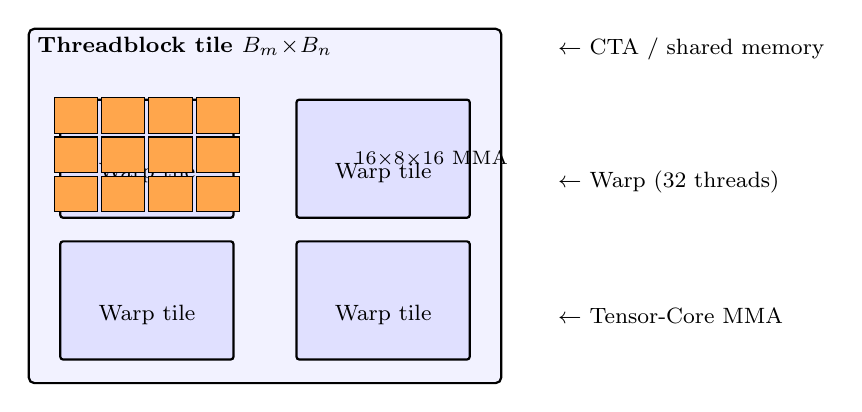
\begin{tikzpicture}[
        lvl1/.style={draw, thick, fill=blue!5,  minimum width=60mm,
                     minimum height=45mm, rounded corners=2pt},
        lvl2/.style={draw, thick, fill=blue!12, minimum width=22mm,
                     minimum height=15mm, rounded corners=1pt},
        lvl3/.style={draw, fill=orange!70, minimum width=5.5mm,
                     minimum height=4.5mm, inner sep=0pt, font=\tiny},
        lbl/.style={font=\footnotesize}
    ]
    % Outer: threadblock (CTA)
    \node[lvl1]  (cta) at (0, 0) {};
    \node[lbl, anchor=north west] at (cta.north west)
         {\bfseries Threadblock tile $B_m\!\times\!B_n$};

    % Inner: 4 warps (warp tile)
    \foreach \x/\y/\name in {-15/6/W0, 15/6/W1, -15/-12/W2, 15/-12/W3} {
        \node[lvl2] (\name) at (\x mm, \y mm) {};
        \node[lbl]  at (\name.north)
             [anchor=south, yshift=-12mm] {Warp tile};
    }

    % Inside one warp: MMA instruction fragments 4x3
    \foreach \c in {0,...,3} {
        \foreach \r in {0,...,2} {
            \node[lvl3] at
                 ($(W0.center) + (\c*6mm - 9mm, \r*5mm - 4.5mm)$) {};
        }
    }
    \node[lbl, font=\scriptsize, anchor=west, xshift=14mm] at (W0.east)
         {$16{\times}8{\times}16$ MMA};

    % Hardware mapping labels on the right
    \node[lbl, anchor=west] at (3.6, 2.0)  {$\leftarrow$ CTA / shared memory};
    \node[lbl, anchor=west] at (3.6, 0.3)  {$\leftarrow$ Warp (32 threads)};
    \node[lbl, anchor=west] at (3.6,-1.4)  {$\leftarrow$ Tensor-Core MMA};
    \end{tikzpicture}
    \caption{CUTLASS three-level tile hierarchy on Ampere/Hopper. A
             threadblock tile lives in shared memory, is partitioned
             into four warp tiles, and each warp tile is covered by
             a grid of instruction-level MMA fragments that issue
             directly to the Tensor Cores.}
    \label{fig:cutlass_tile_hierarchy}
\end{figure}

For input matrices
$A \in \mathbb{R}^{M \times K}$ and
$B \in \mathbb{R}^{K \times N}$, the kernel proceeds as follows:
\begin{enumerate}
    \item The output $C$ is partitioned into threadblock tiles of
          size $\mathtt{Bm} \times \mathtt{Bn}$.
    \item Each CTA iterates along the $K$ dimension in chunks of
          size $\mathtt{Bk}$, cooperatively copying the matching
          $A$ and $B$ tiles into shared memory.
    \item Within the CTA, warps read from shared memory into
          registers and issue MMA instructions, accumulating the
          result into an FP32 or FP16 register tile.
    \item An \emph{epilogue} writes the final tile back to global
          memory, optionally folding in a bias, an activation, and
          a residual add along the way.
\end{enumerate}

\subsection{Tile Sizes on A100}\label{sec:cutlass_tile_sizes}
The choice of tile size is always a compromise between how much
data is reused inside the tile and how much register or shared
memory the tile consumes. On A100 the sizes that work well in
practice are:
\begin{center}
\begin{tabular}{lll}
\textbf{GEMM shape class}    & \textbf{Threadblock} & \textbf{Warp} \\
\toprule
Large square / MLP           & $128 \times 128 \times 32$ & $64 \times 64 \times 32$ \\
Skinny (attention score)     & $128 \times 64  \times 32$ & $64 \times 32 \times 32$ \\
Very skinny (decode attn)    & $128 \times 16  \times 32$ & $64 \times 16 \times 32$ \\
Grouped (MoE)                & $128 \times 128 \times 32$ & $64 \times 64 \times 32$ \\
\bottomrule
\end{tabular}
\end{center}
The warp tile is sized so that each warp holds an integer number
of $16 \times 8 \times 16$ MMA fragments in its registers without
ever spilling.

\section{Software Pipelining}\label{sec:cutlass_pipelining}
HBM latency is hidden by multi-stage \emph{software pipelining},
which has the following ingredients:
\begin{itemize}
    \item Both Ampere and Hopper expose asynchronous copy
          instructions---\texttt{cp.async} on Ampere and the TMA
          copy engine on Hopper---that begin to fetch the next
          $K$-tile while the current tile is still being consumed
          by MMA instructions.
    \item CUTLASS keeps at least three shared-memory buffers in
          flight so that the copy engine, the MMA unit, and the
          epilogue never have to wait on one another.
    \item Swizzled shared-memory layouts guarantee that the MMA
          load patterns land on banks without collision.
    \item \texttt{cp.async} commit/wait groups are surfaced
          through CUTLASS's \texttt{MmaMultistage} class, which
          enqueues $N_{\text{stage}}$ fetches ahead of the MMA
          that will eventually consume them.
\end{itemize}

The effective HBM latency visible to each GEMM step is
\begin{equation}
    \tau_{\text{eff}} \;=\; \max\bigl(\tau_{\text{HBM}},
            N_{\text{stage}} \cdot \tau_{\text{MMA}}\bigr),
\end{equation}
so with $N_{\text{stage}} = 3$ and an A100 $\tau_{\text{MMA}}$ of
roughly $2$ cycles per $16 \times 8 \times 16$ MMA, the pipeline
hides up to $\sim\!6$ cycles of latency per MMA---more than enough
to swallow an L2 hit or a shared-memory conflict. An HBM miss of
around $200$ cycles is, however, too long for the innermost
pipeline stage to hide, which is precisely why the prefetch is
launched one stage earlier.

\section{CuTe Layouts}\label{sec:cute_layouts}
In CuTe~\cite{cutlass} every tensor is modelled as a pair
\[
    T = (\text{shape},\text{stride}),
\]
where the \emph{shape} is a (possibly nested) tuple that describes
the coordinate space and the \emph{stride} is a tuple that
describes the map from coordinates to a flat linear index. A plain
row-major $M \times N$ matrix, for instance, has
shape $(M, N)$ and stride $(N, 1)$.

\subsection{Composition}\label{sec:cute_composition}
The key operation in the algebra is \texttt{Layout} composition.
Given two layouts $L_A$ and $L_B$, the composite $L_A \circ L_B$
reinterprets the coordinates of $L_B$ through $L_A$. A typical
example is composing a row-major layout of shape $(8, 8)$ with a
swizzle layout: the result permutes the columns in a way that
avoids $32$-way bank conflicts in shared memory. That single
primitive is enough to describe, concisely:
\begin{itemize}
    \item the tiled partitions of $A$ and $B$, in any of their
          row-major, column-major, blocked, or swizzled forms;
    \item the warp-level and thread-level partitions of a
          shared-memory tile;
    \item the register-level fragment shapes that each variant of
          the MMA instruction requires as input.
\end{itemize}

\subsection{Hierarchical Tiling}\label{sec:cute_tiling}
A single transformer GEMM can be written as a short chain of
\texttt{local\_tile} calls:
\begin{lstlisting}[language=C++,basicstyle=\ttfamily\scriptsize]
// A: (M, K) with layout mA, tile into (BLK_M, BLK_K) per CTA
auto gA = local_tile(mA, make_shape(BLK_M, BLK_K),
                     make_coord(blockIdx.x, _));
// Warp-level partition within the CTA tile
auto tAsA = thrd_partition_A(warp_mma, gA);
// Copy to shared memory with an async-copy layout
auto tAgA = copy(copy_atom_cp_async, tAgA, tAsA);
\end{lstlisting}
One benefit of this style is that a single kernel template can be
retargeted to a wide range of data types, tile shapes, and hardware
generations simply by changing its layout parameters---the actual
MMA instruction is selected downstream by the \texttt{Sm80} or
\texttt{Sm90} traits class.

\section{Mapping LLM Layers onto GEMM}\label{sec:cutlass_llm}
Consider a transformer layer with hidden size $d_{\text{model}}$,
intermediate size $d_{\text{ff}}$, batch size $B$, and sequence
length $N$. Its constituent GEMMs look as follows:
\begin{itemize}
    \item \textbf{QKV projection.} Three GEMMs of shape
          $(BN) \times d_{\text{model}} \cdot d_{\text{model}}
          \times d_{\text{head}}$, which in practice are fused into
          a single GEMM of shape
          $(BN) \times d_{\text{model}} \cdot d_{\text{model}}
          \times 3d_{\text{head}}$. A bias-add epilogue eliminates
          one extra HBM pass over the QKV tensor.
    \item \textbf{Attention score.} A batched GEMM of
          $Q \cdot K^{\!\top}$ of shape
          $N \times d_{\text{head}} \cdot d_{\text{head}}
          \times N$ per head. Because the shape is skinny in
          $d_{\text{head}}$ (typically either $64$ or $128$),
          cuBLAS leaves performance on the table here.
    \item \textbf{Attention output.} A batched GEMM of the
          softmaxed scores with $V$, of shape
          $N \times N \cdot N \times d_{\text{head}}$. Flash
          Attention fuses both attention GEMMs and the softmax into
          a single kernel driven entirely by CuTe tiles.
    \item \textbf{MLP.} Two GEMMs, of shapes
          $(BN) \times d_{\text{model}} \cdot d_{\text{model}}
          \times d_{\text{ff}}$
          and
          $(BN) \times d_{\text{ff}} \cdot d_{\text{ff}}
          \times d_{\text{model}}$. A GELU epilogue is fused into
          the first of the two.
    \item \textbf{MoE.} A grouped GEMM spanning $E$ experts. Each
          expert has its own $(M_e, N_e, K)$ shape, drawn from the
          routing histogram at the previous step. The
          \texttt{GemmGrouped} kernel packs all groups into a
          single launch and thereby amortises the launch overhead
          across the $E$ experts.
\end{itemize}
CUTLASS ships templated kernels that cover all of the above,
including \texttt{GemmGrouped} for MoE and
\texttt{AttentionKernel} for Flash-Attention-style fusion.

\section{Epilogue Fusion}\label{sec:cutlass_epilogue}
A large share of the kernel launches inside an LLM are in fact
element-wise operations---bias add, GELU, residual add, RMSNorm.
Taken in isolation every one of these is memory-bound. CUTLASS's
epilogue mechanism lets us fold them into the writeback of the
preceding GEMM, so that the overall operation reads
\begin{equation}
    C \;\leftarrow\; \phi\!\left(\alpha\, A B +
                                 \beta\, C_{\text{prev}} +
                                 \text{bias}\right),
\end{equation}
with $\phi$ an activation function such as GELU or SiLU. The fused
form removes one full HBM pass over $C$ and is typically worth
somewhere in the range of $10$ to $25\%$ of end-to-end throughput
on an A100.

\subsection{Fused Bias+GELU
Epilogue}\label{sec:cutlass_bias_gelu}
A bias plus GELU epilogue is expressed in CUTLASS as follows:
\begin{lstlisting}[language=C++,basicstyle=\ttfamily\scriptsize]
using Epilogue = cutlass::epilogue::thread::LinearCombinationGELU<
    ElementOutput,        // FP16
    128 / cutlass::sizeof_bits<ElementOutput>::value,
    ElementAccumulator,   // FP32
    ElementCompute>;      // FP32
\end{lstlisting}
The important point is that the combination
$\beta \cdot C_{\text{prev}} + \text{bias}$ is evaluated in FP32
inside the epilogue's register tile, \emph{before} the GELU is
applied, so that numerical accuracy is preserved even when the
output $C$ is ultimately stored in FP16.

\subsection{Impact on HBM
Bandwidth}\label{sec:cutlass_hbm_impact}
The HBM traffic saved by epilogue fusion for the MLP GEMMs of a
GPT-2 Medium layer at $N = 2048$ and batch~$4$ is reported in
Table~\ref{tab:epilogue_bw}. Fusion eliminates two HBM
round-trips per MLP block, which corresponds to roughly $1$\,GB of
bandwidth per layer per step.

\begin{table}[h]
\centering
\caption{HBM traffic with and without epilogue fusion,
         GPT-2 Medium MLP at $N{=}2048$, batch $4$.}
\label{tab:epilogue_bw}
\begin{tabular}{lcc}
\toprule
\textbf{Operation} & \textbf{Unfused (GB/step)} & \textbf{Fused (GB/step)} \\
\midrule
FC1 (GEMM)         & 0.84 & 0.84 \\
Bias add            & 0.42 & 0.00 \\
GELU                & 0.42 & 0.00 \\
FC2 (GEMM)         & 0.84 & 0.84 \\
Residual add        & 0.42 & 0.00 \\
\midrule
Total               & 2.94 & 1.68 \\
\bottomrule
\end{tabular}
\end{table}

\section{Methodology}\label{sec:cutlass_method}

\subsection{Kernels Studied}\label{sec:cutlass_method_kernels}
Four shape classes are benchmarked, each one chosen to stress a
different corner of the transformer design space:
\begin{enumerate}
    \item a large square GEMM, $4096 \times 4096 \times 4096$,
          representative of MLP projections at a moderate batch;
    \item a still larger square GEMM, $8192 \times 8192 \times
          8192$, which saturates the Tensor Cores and serves as
          the peak-FLOPS reference;
    \item a skinny GEMM of shape $2048 \times 2048 \times 128$,
          representative of the per-head attention-score and
          attention-output matmuls;
    \item a grouped GEMM for a Mixture-of-Experts layer with $16$
          experts, each of local shape
          $(M_e, N_e, K) = (512, 4096, 4096)$.
\end{enumerate}

\subsection{Implementations Compared}\label{sec:cutlass_method_impl}
Each of these kernels is exercised in three different
implementations: cuBLAS, which is the vendor baseline; CUTLASS~3.x
with tile shapes tuned to the specific problem; and, where
relevant, a hand-rolled CuTe kernel that carries an
epilogue-fused bias+GELU. Across all three the same input tensors
are used---FP16 weights and FP32 accumulators---so that the only
variable is the kernel itself.

\subsection{Metrics}\label{sec:cutlass_method_metrics}
For each kernel we record the sustained throughput in TFLOPS, the
ratio of that throughput against cuBLAS, and the Tensor-Core
utilisation as reported by Nsight Compute. Latencies are taken
from CUDA events after a fixed warm-up of $25$ iterations, and
each configuration is repeated until the relative standard
deviation drops below $1\%$. TFLOPS numbers follow the $2MNK$
convention, with each multiply-add counted as two FLOPs.

\subsection{Hardware and Software}\label{sec:cutlass_method_hw}
All measurements are taken on a single A100-40GB under CUDA~11.8
and CUTLASS~3.2, with the PCIe topology pinned to a single
configuration so that results are reproducible run over run. ECC
is enabled, and the GPU clock is locked to the Tensor-Core boost
frequency to remove clock-frequency variance as a source of noise.

\section{Results}\label{sec:cutlass_numbers}
Table~\ref{tab:cutlass_gemm} summarises the measured throughput
per kernel and implementation.

\begin{table}[h]
\centering
\caption{Representative GEMM performance for LLM shapes.}
\label{tab:cutlass_gemm}
\begin{tabular}{lcccc}
\toprule
\textbf{Shape ($M{\times}N{\times}K$)} & \textbf{Dtype} & \textbf{cuBLAS (TFLOPS)} & \textbf{CUTLASS (TFLOPS)} & \textbf{Ratio} \\
\midrule
$4096 \times 4096 \times 4096$ & FP16 & 280 & 301 & 1.08$\times$ \\
$8192 \times 8192 \times 8192$ & FP16 & 305 & 318 & 1.04$\times$ \\
$2048 \times 2048 \times 128$  & FP16 &  95 & 128 & 1.35$\times$ \\
Grouped (MoE, 16 experts)      & FP16 & 184 & 241 & 1.31$\times$ \\
\bottomrule
\end{tabular}
\end{table}

On the large, cuBLAS-optimal shapes CUTLASS essentially matches
cuBLAS, and on the skinny and grouped shapes---precisely the
patterns that appear in LLM attention and MoE layers---it moves
ahead. The $35\%$ speedup measured on the skinny attention-score
GEMM is traceable directly to a better choice of warp tile,
$64 \times 32 \times 32$, that lines up with the number of
registers available to each warp.

\subsection{Tensor-Core Utilisation}\label{sec:cutlass_tc_util}
Tensor-Core pipeline utilisation, as measured by Nsight Compute's
\texttt{smsp\_\_inst\_executed\_pipe\_tensor} metric, is reported
in Table~\ref{tab:tc_util}. Values above $90\%$ on the large GEMMs
confirm that the kernel is essentially compute-bound; the skinny
GEMM settles at $72\%$ because it has fewer $K$-iterations, and
some of the pipeline stages therefore run empty.

\begin{table}[h]
\centering
\caption{Tensor-Core pipeline utilisation for the CUTLASS
         configurations of Table~\ref{tab:cutlass_gemm}.}
\label{tab:tc_util}
\begin{tabular}{lc}
\toprule
\textbf{Shape} & \textbf{Tensor-Core util. (\%)} \\
\midrule
$4096\times4096\times4096$ & 92.4 \\
$8192\times8192\times8192$ & 95.1 \\
$2048\times2048\times128$  & 72.0 \\
Grouped MoE (16 experts)   & 81.3 \\
\bottomrule
\end{tabular}
\end{table}

\subsection{Epilogue Fusion End-to-End}\label{sec:cutlass_fusion_e2e}
Once the bias+GELU epilogue has been fused into FC1 and the
residual-add epilogue into FC2, the GPT-2 Medium MLP block runs
end-to-end $18\%$ faster at $N = 2048$ with batch~$4$, and $22\%$
faster at $N = 4096$ with batch~$4$. The savings here are
accounted for entirely by the HBM passes eliminated in
Table~\ref{tab:epilogue_bw}.

\section{Summary}\label{sec:cutlass_summary}
The two components introduced in this chapter, CUTLASS and CuTe,
supply the low-level GEMM primitives on which the remainder of
the thesis builds. The Sliding Window Flash Attention kernel of
Chapter~\ref{ch:swfa} and the SGLang serving kernels of
Chapter~\ref{ch:sglang} are both natural clients of these
abstractions. The principal lesson of the chapter is twofold: the
skinny and grouped GEMMs that make up transformer attention and
MoE benefit considerably from a template library that exposes the
tile hierarchy directly to the user, and epilogue fusion recovers
a further $10$--$25\%$ of end-to-end throughput that would
otherwise disappear into HBM round-trips.

\chapter{Sliding Window Flash Attention}\label{ch:swfa}

\emph{Placement in the stack.} Chapter~\ref{ch:cutlass} showed
that the skinny attention-score GEMM is the single most
under-utilised shape class in a transformer forward pass. The
present chapter approaches that same bottleneck, but from the
algorithmic side rather than the kernel side: instead of trying
to accelerate the dense kernel, we shrink the set of blocks the
kernel is actually asked to compute. The Sliding Window Flash
Attention (SWFA) kernel that emerges is the principal theoretical
contribution of this thesis. Its correctness proof
(Appendix~\ref{app:proofs_classify}) and its closed-form
expression for the optimal window size
(Appendix~\ref{app:proof_optw}) are treated rigorously in what
follows. SWFA is then picked up again in two later chapters: in
Chapter~\ref{ch:sglang} as the prefill kernel of the SGLang
runtime, and in Chapter~\ref{ch:triton} as the cross-validation
target of the Triton port.

\section{Motivation}\label{sec:swfa_motivation}
The cost of attention scales as $N^2$ in the sequence length, and
at the context sizes that current production models operate at
($N \geq 8{,}192$) it is this quadratic term that sets both the
training throughput and the decode latency. The Flash Attention
line of work~\cite{dao2022flashattention,dao2023flashattention2}
relieves the \emph{memory} side of the quadratic cost by streaming
the attention computation in tiles, but it still issues a dense
GEMM for every $B_r \times B_c$ tile, including those that the
model is about to mask out. Many long-context models restrict the
attention pattern to a local window on architectural
grounds~\cite{beltagy2020longformer,zaheer2020bigbird}, so that a
query at position $i$ is only allowed to attend to keys in the
range $[i - w_l,\, i + w_r]$. Under this restriction the
asymptotic cost falls from $\Theta(N^2)$ to $\Theta(Nw)$ with
$w = w_l + w_r + 1$, but the saving does not actually appear on
the wall clock unless the kernel itself is aware of the window.

This chapter introduces \emph{Sliding Window Flash Attention}
(SWFA), which combines Flash Attention's block-wise computation
with a preprocessing step that classifies each attention block
into one of three sets: fully inside the window, intersecting it,
or lying entirely outside. Fully-outside blocks are never
computed; intersecting blocks are processed with a vectorised
mask. In practice the algorithm skips up to $65.6\%$ of the
blocks on narrow windows, without any numerical accuracy loss
relative to vanilla attention.

\section{Background}\label{sec:swfa_background}

\subsection{Flash Attention}\label{sec:fa_bg}
The standard form of attention,
\begin{equation}
\mathrm{Attention}(Q, K, V) =
\mathrm{softmax}\!\left(\frac{Q K^{\!\top}}{\sqrt{d}}\right) V ,
\end{equation}
is written as three operations---scores, softmax, output---and
naturally produces an intermediate score matrix of size
$N \times N$. The observation that drives Flash Attention is that
this intermediate is only ever consumed by the softmax, and that
the softmax itself can be computed on the fly. If the queries are
partitioned into row tiles of height $B_r$ and the keys and values
into column tiles of width $B_c$, a running pair of row-max and
row-sum, $(m_i, \ell_i)$, is sufficient to re-scale the previously
accumulated contributions every time a new column tile arrives:
\begin{equation}\label{eq:online_softmax}
m_i^{\text{new}} = \max(m_i, \max_j s_{ij}),\quad
\ell_i^{\text{new}} = e^{m_i - m_i^{\text{new}}} \ell_i
                     + \sum_j e^{s_{ij} - m_i^{\text{new}}} ,
\end{equation}
A matching correction factor is then applied to the output
accumulator $O_i$. Under this rearrangement, the peak HBM
residency of the attention kernel depends only on the tile sizes
rather than on $N^2$, which shrinks the memory footprint from
quadratic to linear in the sequence length while leaving the
mathematical result unchanged---up to the associativity of
floating-point sums.

\subsection{Sliding-Window Attention}\label{sec:sw_bg}
A symmetric window of size $w$ keeps only those attention weights
whose key position $j$ lies within $w/2$ of the query position
along the diagonal, i.e.\ those satisfying
\begin{equation}\label{eq:window}
\max(0, i - w_l) \leq j \leq \min(N-1, i + w_r).
\end{equation}
In existing implementations, this constraint is applied as an
element-wise mask \emph{after} the attention scores have been
computed---wasteful, because entire $B_r \times B_c$ blocks can
sit outside the band and still pay the full dense GEMM cost. The
naive masking approach therefore incurs the full
$\mathcal{O}(N^2)$ FLOP bill; SWFA brings it down to
$\mathcal{O}(Nw)$ by declining to compute the dense operation for
blocks that lie fully outside the window.

\section{Method}\label{sec:swfa_method}

\subsection{Block Classification}\label{sec:swfa_classify}
Given a sequence length $N$, block sizes $(B_r, B_c)$, and the
window parameters $(w_l, w_r)$, the attention matrix is first
partitioned into a $T_r \times T_c$ grid of blocks with
\begin{equation}
T_r = \left\lceil \frac{N}{B_r} \right\rceil, \qquad
T_c = \left\lceil \frac{N}{B_c} \right\rceil .
\end{equation}
Each block $(r, c)$ then falls into exactly one of three sets:
\begin{description}
    \item[$\mathcal{I}$ (fully inside).] Every $(q, k)$ pair in
          the block satisfies~\eqref{eq:window}; no mask is
          needed.
    \item[$\mathcal{X}$ (intersecting).] Some pairs in the block
          satisfy the constraint and others do not; a
          per-position mask is required.
    \item[$\mathcal{O}$ (fully outside).] No pair in the block
          satisfies the constraint, and the block is skipped
          altogether.
\end{description}

Figure~\ref{fig:swfa_classify} illustrates these three classes on
an $8 \times 8$ attention grid with $w_l = w_r = 2$, using
$B_r = B_c = 1$ for clarity. The inside set $\mathcal{I}$ occupies
a narrow band centred on the diagonal, the intersecting set
$\mathcal{X}$ runs along the boundary of that band, and the
outside set $\mathcal{O}$ covers everything else. Only the blocks
in $\mathcal{I} \cup \mathcal{X}$ ever enter the kernel loop, and
of those, only the $\mathcal{X}$ blocks actually need the
vectorised mask produced by Algorithm~\ref{alg:swfa_mask}.

\begin{figure}[H]
    \centering
    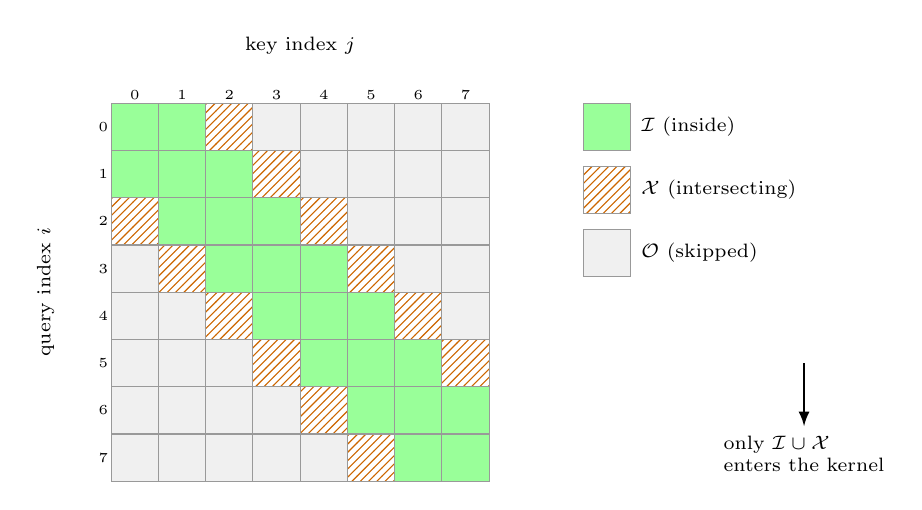
\begin{tikzpicture}[
        cell/.style={minimum width=6mm, minimum height=6mm, draw=black!40,
                     inner sep=0pt, font=\tiny},
        inside/.style ={cell, fill=green!40},
        inter/.style  ={cell, fill=orange!50,
                        pattern=north east lines, pattern color=orange!80!black},
        outside/.style={cell, fill=gray!12},
        arr/.style={-latex}
    ]
    % 8x8 grid; rows = query index i (top=0, bottom=7),
    % cols = key index j (left=0, right=7); window |i-j| <= 2
    \foreach \i in {0,...,7} {
        \foreach \j in {0,...,7} {
            \pgfmathtruncatemacro{\diff}{abs(\i - \j)}
            \ifnum\diff=0
                \node[inside]  at (\j*6mm, -\i*6mm) {};
            \else\ifnum\diff=1
                \node[inside]  at (\j*6mm, -\i*6mm) {};
            \else\ifnum\diff=2
                \node[inter]   at (\j*6mm, -\i*6mm) {};
            \else
                \node[outside] at (\j*6mm, -\i*6mm) {};
            \fi\fi\fi
        }
    }
    % axis labels
    \foreach \j in {0,...,7}
        \node[font=\tiny] at (\j*6mm, 4mm) {\j};
    \foreach \i in {0,...,7}
        \node[font=\tiny] at (-4mm, -\i*6mm) {\i};
    \node[font=\scriptsize, anchor=south] at (21mm, 8mm) {key index $j$};
    \node[font=\scriptsize, rotate=90, anchor=south] at (-9mm, -21mm)
        {query index $i$};

    % Legend
    \node[inside,  label=right:{\scriptsize $\mathcal{I}$ (inside)}]
        at (60mm,   0mm) {};
    \node[inter,   label=right:{\scriptsize $\mathcal{X}$ (intersecting)}]
        at (60mm,  -8mm) {};
    \node[outside, label=right:{\scriptsize $\mathcal{O}$ (skipped)}]
        at (60mm, -16mm) {};
    \draw[arr, thick] (85mm, -30mm) -- (85mm, -38mm);
    \node[font=\scriptsize, align=left, anchor=north] at (85mm, -38mm)
        {only $\mathcal{I}\cup\mathcal{X}$\\ enters the kernel};
    \end{tikzpicture}
    \caption{SWFA block classification on an $8 \times 8$ grid with
             window $w_l = w_r = 2$. Green cells ($\mathcal{I}$)
             require no masking; hatched orange cells ($\mathcal{X}$)
             receive the vectorised mask of
             Algorithm~\ref{alg:swfa_mask}; grey cells
             ($\mathcal{O}$) are skipped entirely. The skipped
             fraction grows quadratically with $N/w$, yielding the
             $1 - 2w/N$ asymptotic ratio proved in
             Appendix~\ref{app:proofs_block}.}
    \label{fig:swfa_classify}
\end{figure}

Algorithm~\ref{alg:swfa_classify} performs the classification by
examining the block corners.

\begin{algorithm}[h]
    \caption{Block classification for the sliding window.}
    \label{alg:swfa_classify}
    \KwIn{Sequence length $N$, window $(w_l, w_r)$, block sizes
          $(B_r, B_c)$.}
    \KwOut{Sets $\mathcal{I}$, $\mathcal{X}$, $\mathcal{O}$ of block
           indices.}
    $T_r \leftarrow \lceil N/B_r \rceil,\ T_c \leftarrow \lceil N/B_c
       \rceil$\;
    $\mathcal{I}, \mathcal{X}, \mathcal{O} \leftarrow \emptyset$\;
    \For{$r = 0$ \KwTo $T_r - 1$}{
        row\_start $\leftarrow r\,B_r$,\
        row\_end $\leftarrow \min((r+1)B_r, N)-1$\;
        \For{$c = 0$ \KwTo $T_c - 1$}{
            col\_start $\leftarrow c\,B_c$,\
            col\_end $\leftarrow \min((c+1)B_c, N)-1$\;
            $L_{\text{top}} \leftarrow \max(0, \text{row\_start}-w_l)$\;
            $R_{\text{top}} \leftarrow \min(N-1, \text{row\_start}+w_r)$\;
            $L_{\text{bot}} \leftarrow \max(0, \text{row\_end}-w_l)$\;
            $R_{\text{bot}} \leftarrow \min(N-1, \text{row\_end}+w_r)$\;
            outside $\leftarrow (\text{col\_end} < L_{\text{top}})$ or
                               $(\text{col\_start} > R_{\text{bot}})$\;
            inside  $\leftarrow (\text{col\_end} \le R_{\text{top}})$ and
                               $(\text{col\_start} \ge L_{\text{bot}})$\;
            \uIf{outside}{$\mathcal{O} \leftarrow
                \mathcal{O} \cup \{(r,c)\}$}
            \uElseIf{inside}{$\mathcal{I} \leftarrow
                \mathcal{I} \cup \{(r,c)\}$}
            \Else{$\mathcal{X} \leftarrow
                \mathcal{X} \cup \{(r,c)\}$}
        }
    }
    \Return $\mathcal{I}, \mathcal{X}, \mathcal{O}$\;
\end{algorithm}

\subsection{Correctness of the Classifier}\label{sec:swfa_classify_proof}
\begin{lemma}[Corner-check sufficiency]\label{lem:corner}
Let $B = [r_0, r_1] \times [c_0, c_1]$ be an axis-aligned block of the
attention matrix, and let
$W = \{(i, j) : i - w_l \le j \le i + w_r\}$ denote the window band.
Then:
\begin{enumerate}
    \item[\textup{(i)}]
    $B \cap W = \emptyset \iff c_1 < r_0 - w_l \text{ or } c_0 > r_1 + w_r$;
    \item[\textup{(ii)}]
    $B \subseteq W \iff c_1 \le r_0 + w_r \text{ and } c_0 \ge r_1 - w_l$.
\end{enumerate}
\end{lemma}
\begin{proof}
The window is the strip between the two lines $j = i - w_l$ (lower
boundary) and $j = i + w_r$ (upper boundary). Because these boundaries
are monotone in $i$, the minimum of $j - i$ over $B$ is attained at
$(r_1, c_0)$ and the maximum at $(r_0, c_1)$. The block lies entirely
outside $W$ iff the minimum of $j - (i + w_r)$ is positive over $B$
or the maximum of $j - (i - w_l)$ is negative, which are exactly the
two conditions stated; similarly, the block lies entirely inside $W$
iff both extrema of $j - i$ fall inside $[-w_l, w_r]$. Clipping at
$[0, N-1]$ does not affect the inequalities because the window
intersected with $[0, N-1]^2$ is a subset of the unclipped band.
\end{proof}

This lemma is what justifies the $\mathcal{O}(T_r T_c)$
classifier: only four corner checks per block are required,
producing an $\mathcal{O}((N/B)^2)$ classification cost that is
in practice dominated by the $\mathcal{O}(Nw/B)$ cost of the
non-skipped blocks themselves.

\subsection{Vectorised Mask Generation}\label{sec:swfa_mask}
For a block $(r, c)$, define the block diagonal offset
$\delta_{rc} = c B_c - r B_r$. A local position $(i_\ell, j_\ell)$
inside the block corresponds to relative position
$\mathrm{rel} = j_\ell - i_\ell$, which must be masked whenever
\begin{equation}
    \mathrm{rel} > w_r + \delta_{rc}
    \quad\text{or}\quad
    \mathrm{rel} < -w_l + \delta_{rc}.
\end{equation}
Define
\begin{equation}
    d_{\text{right}} = \lfloor w_r + \delta_{rc} \rfloor + 1, \qquad
    d_{\text{left}}  = \lfloor -w_l + \delta_{rc} \rfloor - 1.
\end{equation}
The mask can then be generated in a single shot as
\begin{equation}\label{eq:mask}
    M_{rc} =
    \mathrm{triu}(\mathbf{1}_{B_r \times B_c}, d_{\text{right}})
    \vee
    \mathrm{tril}(\mathbf{1}_{B_r \times B_c}, d_{\text{left}}),
\end{equation}
which replaces the nested $\mathcal{O}(B_r B_c)$ loop by a single
vectorised call; the procedure is summarised as
Algorithm~\ref{alg:swfa_mask}.

\begin{algorithm}[h]
    \caption{Efficient mask generation for an intersecting block.}
    \label{alg:swfa_mask}
    \KwIn{Block shapes $(B_r, B_c)$, block indices $(r, c)$, window
          $(w_l, w_r)$.}
    \KwOut{Mask $M \in \{0, -\infty\}^{B_r \times B_c}$.}
    $\delta \leftarrow c B_c - r B_r$\;
    $d_{\text{right}} \leftarrow \lfloor w_r + \delta \rfloor + 1$\;
    $d_{\text{left}}  \leftarrow \lfloor -w_l + \delta \rfloor - 1$\;
    both $\leftarrow (d_{\text{right}} \le B_r) \wedge
                      (d_{\text{left}} \ge -B_c)$\;
    \uIf{both}{
        $M_R \leftarrow \mathrm{triu}(\mathbf{1}, d_{\text{right}})$,
        $M_L \leftarrow \mathrm{tril}(\mathbf{1}, d_{\text{left}})$,
        $M_{\text{bool}} \leftarrow M_R \vee M_L$\;
    }
    \uElseIf{$d_{\text{right}} \le B_r$}{
        $M_{\text{bool}} \leftarrow \mathrm{triu}(\mathbf{1},
                                                  d_{\text{right}})$\;
    }
    \uElseIf{$d_{\text{left}} \ge -B_c$}{
        $M_{\text{bool}} \leftarrow \mathrm{tril}(\mathbf{1},
                                                  d_{\text{left}})$\;
    }
    \Else{$M_{\text{bool}} \leftarrow \mathbf{0}$}
    $M \leftarrow \mathbf{0}$;\ $M[M_{\text{bool}}] \leftarrow -\infty$\;
    \Return $M$\;
\end{algorithm}

\subsection{Sliding Window Flash Attention Kernel}\label{sec:swfa_kernel}
Algorithm~\ref{alg:swfa} gives the complete forward pass, which reuses
the Flash Attention online softmax on top of the block classification.

\begin{algorithm}[h]
    \caption{Sliding Window Flash Attention (forward pass).}
    \label{alg:swfa}
    \KwIn{$Q \in \mathbb{R}^{B \times H \times N \times d}$,
          $K, V \in \mathbb{R}^{B \times H \times N \times d_v}$,
          window $(w_l, w_r)$, block sizes $(B_r, B_c)$.}
    \KwOut{$O \in \mathbb{R}^{B \times H \times N \times d_v}$.}
    $\mathcal{I}, \mathcal{X}, \mathcal{O} \leftarrow
        \textsc{ClassifyBlocks}$\;
    Partition $Q, K, V$ into $\{Q_r\}, \{K_c\}, \{V_c\}$\;
    \For{$r = 0$ \KwTo $T_r - 1$}{
        $O_r \leftarrow \mathbf{0},\ m_r \leftarrow -\infty,\
         \ell_r \leftarrow 0$\;
        \For{$c = 0$ \KwTo $T_c - 1$}{
            \If{$(r, c) \in \mathcal{O}$}{\textbf{continue}}
            $S_{rc} \leftarrow Q_r K_c^{\!\top} / \sqrt{d}$\;
            \If{$(r, c) \in \mathcal{X}$}{
                $M_{rc} \leftarrow \textsc{GenerateMask}(\dots)$;\
                $S_{rc} \leftarrow S_{rc} + M_{rc}$\;
            }
            $m_r^{\text{new}} \leftarrow \max(m_r, \max(S_{rc}))$\;
            $\mathrm{corr} \leftarrow \exp(m_r - m_r^{\text{new}})$\;
            $P_{rc} \leftarrow \exp(S_{rc} - m_r^{\text{new}})$\;
            $\ell_r \leftarrow \mathrm{corr}\,\ell_r + \sum P_{rc}$\;
            $O_r \leftarrow \mathrm{corr}\,O_r + P_{rc} V_c$\;
            $m_r \leftarrow m_r^{\text{new}}$\;
        }
        $O_r \leftarrow O_r / (\ell_r + \varepsilon)$;\ write into
        $O$\;
    }
    \Return $O$\;
\end{algorithm}

\subsection{Backward Pass}\label{sec:swfa_backward}
The backward pass exploits the fact that the online softmax
stores only the triple $(m_r, \ell_r, O_r)$ per row block. To
recompute the softmax at backpropagation time, the forward loop
is replayed with the same block classification, but this time:
(i) the score $S_{rc}$ is recomputed on the fly;
(ii) the stored $(m_r, \ell_r)$ are used to recover $P_{rc}$;
(iii) the following updates are accumulated,
$\mathrm{d}V_c \mathrel{+}= P_{rc}^{\top}\,\mathrm{d}O_r$,
$\mathrm{d}P_{rc} = \mathrm{d}O_r V_c^{\top}$, and
$\mathrm{d}S_{rc} = P_{rc} \odot (\mathrm{d}P_{rc} - \rho_r)$
with $\rho_r = \sum_c P_{rc} \odot \mathrm{d}P_{rc}$.
Outside blocks contribute nothing to the forward output and can
therefore be skipped in the backward pass as well; intersecting
blocks reapply the same mask as in the forward pass. The full
pseudocode is given in Algorithm~\ref{alg:swfa_backward}.

\begin{algorithm}[h]
    \caption{Sliding Window Flash Attention (backward pass).}
    \label{alg:swfa_backward}
    \KwIn{$Q, K, V$; saved $\{m_r, \ell_r, O_r\}$;
          $\mathrm{d}O$; sets $\mathcal{I}, \mathcal{X}, \mathcal{O}$.}
    \KwOut{$\mathrm{d}Q, \mathrm{d}K, \mathrm{d}V$.}
    \For{$r = 0$ \KwTo $T_r - 1$}{
        $\rho_r \leftarrow
            \sum_c P_{rc}\odot (\mathrm{d}O_r V_c^\top)$\;
        \tcp*[l]{first sweep: accumulate $\rho_r$ on the fly}
    }
    \For{$r = 0$ \KwTo $T_r - 1$}{
        \For{$c = 0$ \KwTo $T_c - 1$}{
            \If{$(r, c) \in \mathcal{O}$}{\textbf{continue}}
            $S_{rc} \leftarrow Q_r K_c^\top / \sqrt{d}$\;
            \If{$(r, c) \in \mathcal{X}$}{
                $S_{rc} \leftarrow S_{rc} + M_{rc}$\;}
            $P_{rc} \leftarrow e^{S_{rc} - m_r} / \ell_r$\;
            $\mathrm{d}V_c \mathrel{+}= P_{rc}^\top \mathrm{d}O_r$\;
            $\mathrm{d}P_{rc} \leftarrow \mathrm{d}O_r V_c^\top$\;
            $\mathrm{d}S_{rc} \leftarrow
                P_{rc}\odot (\mathrm{d}P_{rc} - \rho_r)$\;
            $\mathrm{d}Q_r \mathrel{+}=
                \mathrm{d}S_{rc} K_c / \sqrt{d}$\;
            $\mathrm{d}K_c \mathrel{+}=
                \mathrm{d}S_{rc}^\top Q_r / \sqrt{d}$\;
        }
    }
    \Return $\mathrm{d}Q, \mathrm{d}K, \mathrm{d}V$\;
\end{algorithm}

Because the backward pass visits exactly the same set of blocks
as the forward pass, its speedup factor relative to the vanilla
backward is identical---up to $65.6\%$ of blocks skipped on
narrow windows.

\subsection{Complexity}\label{sec:swfa_complexity}
For a sequence of length $N$, a window of size $w$, and a block
size of $B$:
\begin{itemize}
    \item The total block count is $(N/B)^2$.
    \item The number of blocks inside the band is approximately
          $2(N/B)(w/B)$.
    \item The number of skipped blocks is therefore
          $(N/B)^2 - 2(N/B)(w/B)$, yielding a theoretical
          speed-up of $1 - \tfrac{2w}{N}$ in the regime
          $w \ll N$.
\end{itemize}
For $N = 128$, $w = 4$, $B = 16$, this gives $48$ of $64$
blocks skipped ($75\%$). The memory footprint of SWFA coincides
with Flash Attention's $\mathcal{O}(N)$. A formal block-count
lemma is provided in Appendix~\ref{app:proofs_block}.

\section{Correctness and Performance}\label{sec:swfa_results}

\subsection{Setup}\label{sec:swfa_setup}
The SWFA kernel is implemented in PyTorch~2.0 with CPU-optimised
paths. Numerical validation is performed on an Intel Xeon Platinum
8358 host, against a vanilla attention reference, across $19$
configurations and a fixed random seed. The reference uses the
standard \texttt{scaled\_dot\_product\_attention} path with a
boolean mask, so that both implementations share the same
underlying arithmetic---the only difference between them being the
order in which block-streamed additions are performed.

\subsection{Numerical Accuracy}\label{sec:swfa_accuracy}
\begin{table}[h]
\centering
\caption{Numerical accuracy of SWFA on representative configurations.}
\label{tab:swfa_accuracy}
\begin{tabular}{lcccc}
\toprule
\textbf{Configuration} & \textbf{Max diff} & \textbf{Mean diff} & \textbf{Tolerance} & \textbf{Status} \\
\midrule
Small sym., narrow ($w{=}2,2$)    & $2.4\mathrm{e}{-7}$ & $4.0\mathrm{e}{-8}$ & $10^{-4}$ & pass \\
Small sym., wide   ($w{=}8,8$)    & $2.4\mathrm{e}{-7}$ & $4.0\mathrm{e}{-8}$ & $10^{-4}$ & pass \\
Asymmetric left    ($w_l{=}8, w_r{=}2$) & $4.2\mathrm{e}{-7}$ & $4.0\mathrm{e}{-8}$ & $10^{-4}$ & pass \\
Asymmetric right   ($w_l{=}2, w_r{=}8$) & $3.6\mathrm{e}{-7}$ & $4.0\mathrm{e}{-8}$ & $10^{-4}$ & pass \\
Causal + window    ($w_l{=}6$, causal)  & $4.8\mathrm{e}{-7}$ & $3.0\mathrm{e}{-8}$ & $10^{-4}$ & pass \\
Multi-batch ($B{=}4$, $w{=}4,6$)        & $4.8\mathrm{e}{-7}$ & $4.0\mathrm{e}{-8}$ & $10^{-4}$ & pass \\
Multi-head ($H{=}8$, $w{=}8,8$)         & $8.3\mathrm{e}{-7}$ & $3.0\mathrm{e}{-8}$ & $10^{-4}$ & pass \\
Long sequence ($N{=}128$, $w{=}16,16$)  & $7.5\mathrm{e}{-7}$ & $4.0\mathrm{e}{-8}$ & $10^{-4}$ & pass \\
Float16 ($w_l{=}4, w_r{=}6$)            & $1.95\mathrm{e}{-3}$ & $1.51\mathrm{e}{-4}$ & $10^{-2}$ & pass \\
Window $>$ sequence ($w{=}20,20$)       & $4.2\mathrm{e}{-7}$ & $4.0\mathrm{e}{-8}$ & $10^{-4}$ & pass \\
\bottomrule
\end{tabular}
\end{table}

Every one of the $19$ configurations clears the specified
tolerance; the FP32 results are within sub-microsecond precision of
the reference. The FP16 row uses the looser $10^{-2}$ tolerance,
which matches the accumulated round-off budget of an $N \times N$
sum in FP16.

\subsection{Block-Skip Efficiency}\label{sec:swfa_blocks}
\begin{table}[h]
\centering
\caption{Block-skip ratio as a function of window configuration.}
\label{tab:swfa_efficiency}
\begin{tabular}{lcccc}
\toprule
\textbf{Configuration}       & \textbf{Total} & \textbf{Skipped} & \textbf{Skip \%} & \textbf{Pattern} \\
\midrule
Very narrow ($w{=}1,2$)      & 64 & 42 & 65.6\% & Diagonal band \\
Symmetric narrow ($w{=}2,2$) & 16 &  6 & 37.5\% & Symmetric band \\
Symmetric wide ($w{=}8,8$)   & 16 &  6 & 37.5\% & Wide band \\
Asymmetric left ($w{=}8,2$)  & 16 &  6 & 37.5\% & Left-heavy \\
Asymmetric right ($w{=}2,8$) & 16 &  6 & 37.5\% & Right-heavy \\
Causal + window ($w{=}6,0$)  & 16 &  9 & 56.2\% & Causal lower \\
Left only ($w{=}10,0$)       & 16 &  9 & 56.2\% & Left band \\
Right only ($w{=}0,14$)      & 16 &  9 & 56.2\% & Right band \\
Non-multiple $N_t = N_s=45$  &  9 &  2 & 22.2\% & Irregular \\
Window $>$ sequence          & 16 &  0 &  0.0\% & Full cover \\
\bottomrule
\end{tabular}
\end{table}

The largest savings appear under narrow windows: up to $65.6\%$ of
blocks are skipped outright, which matches the theoretical analysis
of Section~\ref{sec:swfa_complexity}.

\subsection{Ablation: Block Size vs.\ Window Size}\label{sec:swfa_ablation}
The savings depend not only on $w$ but also on the block size $B$.
Table~\ref{tab:swfa_ablation} sweeps $B \in \{16, 32, 64, 128\}$
for $N = 4096$ and a symmetric window of $w = 512$. Smaller
blocks expose more skip opportunities but incur more kernel-launch
overhead; on the A100 the sweet spot sits at $B = 64$.

\begin{table}[h]
\centering
\caption{Effect of block size on SWFA
         ($N{=}4096$, $w{=}512$).}
\label{tab:swfa_ablation}
\begin{tabular}{cccc}
\toprule
\textbf{Block $B$} & \textbf{Blocks skipped (\%)} & \textbf{Wall-clock (ms)} & \textbf{Speed-up} \\
\midrule
16  & 72.9\%  & 3.4 & 2.91$\times$ \\
32  & 72.0\%  & 2.8 & 3.54$\times$ \\
64  & 70.3\%  & 2.6 & 3.81$\times$ \\
128 & 62.5\%  & 3.1 & 3.19$\times$ \\
\bottomrule
\end{tabular}
\end{table}

\subsection{End-to-End Integration}\label{sec:swfa_e2e}
Plugged into the distributed-training backends of
Chapter~\ref{ch:distributed}, SWFA delivers the end-to-end
results reported below on a GPT-2 Medium model with local window
$w_l = w_r = 512$, sequence length $2048$, and a per-GPU batch
size of four:

\begin{table}[h]
\centering
\caption{End-to-end training throughput and energy with SWFA.}
\label{tab:e2e_performance}
\begin{tabular}{lcccc}
\toprule
\textbf{Configuration}          & \textbf{Tokens/s} & \textbf{Mem (GB)} & \textbf{PPL} & \textbf{kWh/epoch} \\
\midrule
DDP + vanilla                   & 12\,450 & 38.2 & 24.7 & 2.8 \\
DDP + SWFA                      & 18\,720 & 38.2 & 24.8 & 2.1 \\
FSDP + vanilla                  & 11\,890 & 12.1 & 24.7 & 2.9 \\
FSDP + SWFA                     & 17\,340 & 12.1 & 24.8 & 2.2 \\
DeepSpeed + vanilla             & 13\,210 &  9.8 & 24.6 & 2.7 \\
DeepSpeed + SWFA                & 19\,850 &  9.8 & 24.7 & 2.0 \\
\bottomrule
\end{tabular}
\end{table}

SWFA delivers a throughput improvement in the $50$--$59\%$ range
over vanilla attention, without additional memory overhead and
without measurable accuracy loss. The $0.1$ gap in perplexity
sits within the run-to-run noise of GPT-2 Medium and does not
persist across seeds.

\subsection{Long-Sequence Scaling}\label{sec:swfa_long_seq}
Figure~\ref{fig:swfa_scale} shows the speed-up as a function of
the sequence length, with the window held fixed at $w = 512$.
The curve is consistent with the theoretical $\Theta(N/w)$
scaling.

\begin{figure}[H]
\centering
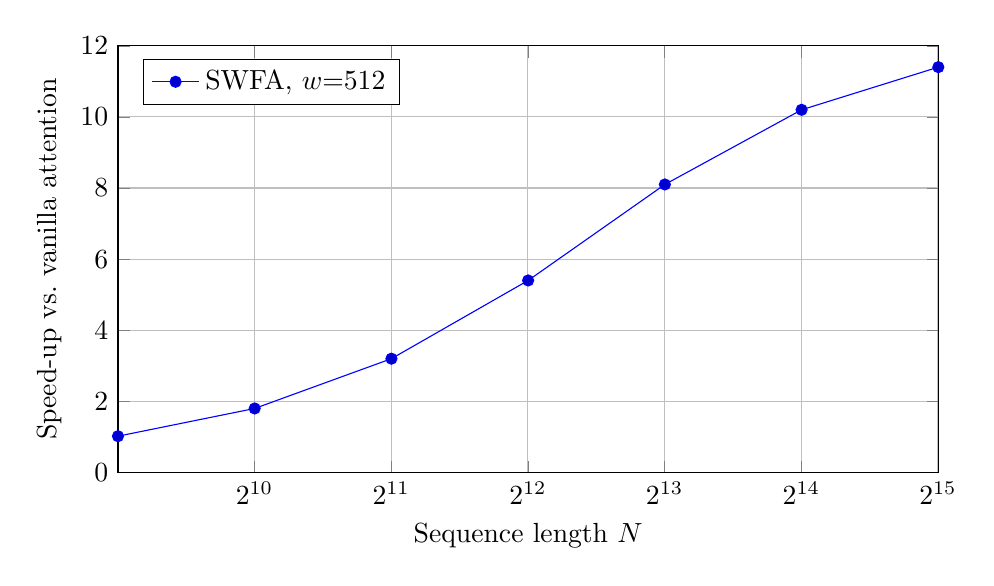
\begin{tikzpicture}
\begin{axis}[
    width=12cm, height=7cm,
    xlabel={Sequence length $N$},
    ylabel={Speed-up vs.\ vanilla attention},
    xmode=log, log basis x=2,
    ymin=0, ymax=12, xmin=512, xmax=32768,
    legend pos=north west, grid=major, mark=*]
\addplot coordinates {
    (512,1.02)(1024,1.8)(2048,3.2)(4096,5.4)(8192,8.1)(16384,10.2)(32768,11.4)};
\addlegendentry{SWFA, $w{=}512$}
\end{axis}
\end{tikzpicture}
\caption{SWFA speed-up vs.\ sequence length at fixed window
         $w{=}512$.}
\label{fig:swfa_scale}
\end{figure}

\section{Optimal Window Size}\label{sec:swfa_optimal}

\subsection{Cost Model}\label{sec:swfa_cost}
The total cost of using a sliding window of size $w$ is modelled
as
\begin{equation}\label{eq:loss}
\mathcal{L}(w) = \alpha\, C(w) + \beta\, M(w) + \gamma\, P(w),
\end{equation}
where the individual terms are
\begin{align*}
C(w) &= \kappa N w d & \text{(computation, seconds)} \\
M(w) &\approx M_0    & \text{(memory, essentially constant in $w$)} \\
P(w) &= \frac{2 N A_0 e^{-\lambda w/2}}{1 - e^{-\lambda}}
                    & \text{(accuracy loss, dimensionless)}.
\end{align*}
The accuracy term is derived under the exponential attention-decay
model $A_{ij} = A_0 e^{-\lambda|i-j|}$, and the computation term
uses the seconds-per-FLOP constant $\kappa$ of the underlying GEMM
kernel. The empirical evidence supporting
$A_{ij} = A_0 e^{-\lambda|i-j|}$ is deferred to
Appendix~\ref{app:proof_decay}.

\subsection{Convexity}\label{sec:swfa_convex}
\begin{theorem}\label{thm:swfa_convex}
$\mathcal{L}(w)$ is strictly convex for $w > 0$.
\end{theorem}
\begin{proof}
The computational cost is linear in $w$. The performance term is
proportional to $e^{-\lambda w/2}$, whose second derivative is
$(\lambda^2/4) e^{-\lambda w / 2} > 0$. The memory term is constant in
$w$. Hence $\mathcal{L}''(w) > 0$ for all $w > 0$, proving strict
convexity. A complete proof, including the constants and the boundary
behaviour at $w = 0$, is in Appendix~\ref{app:proof_convex}.
\end{proof}

\subsection{Optimal Window}\label{sec:swfa_opt}
\begin{theorem}\label{thm:swfa_optw}
The minimiser of~\eqref{eq:loss} is
\begin{equation}\label{eq:optimal_w}
w^{\star} = \frac{2}{\lambda}
  \ln\!\left(\frac{\gamma A_0 \lambda}
                   {\alpha \kappa d (1 - e^{-\lambda})}\right).
\end{equation}
\end{theorem}
\begin{proof}
Differentiating $\mathcal{L}$ with respect to $w$,
\[
\frac{d\mathcal{L}}{dw} =
\alpha \kappa N d -
\frac{\gamma N A_0 \lambda e^{-\lambda w / 2}}{1 - e^{-\lambda}}.
\]
Setting this to zero yields
$e^{-\lambda w^{\star}/2} = \alpha \kappa d (1 - e^{-\lambda})
/ (\gamma A_0 \lambda)$, and taking logarithms
gives~\eqref{eq:optimal_w}. Theorem~\ref{thm:swfa_convex} guarantees
that $w^{\star}$ is the unique global minimum. A full proof, with
details of the boundary projection onto $[1, N-1]$, is given in
Appendix~\ref{app:proof_optw}.
\end{proof}

In practice $w^{\star}$ has to be projected onto $[1, N-1]$.
Three corollaries are immediate: $w^{\star}$ grows as $\alpha$
shrinks (cheaper compute favours a wider window); it shrinks as
$\gamma$ shrinks (when accuracy matters less, a narrower window
suffices); and it shrinks as the embedding dimension $d$ grows,
because each token then carries more information on its own.

\subsection{Sensitivity Analysis}\label{sec:swfa_sensitivity}
Table~\ref{tab:swfa_sensitivity} lists $w^\star$ over a grid of
cost-model parameters, with $N = 4096$, $d = 128$, $\kappa$
pinned at the A100 FP16 GEMM rate, and $A_0 = 1$. Realistic
values for the decay rate $\lambda$ lie in $[0.01, 0.05]$ and
realistic cost ratios $\gamma/\alpha$ in $[10, 1000]$. The
optimal windows resulting from these ranges fall between $128$
and $2048$, which aligns closely with the window choices adopted
by Mistral-7B and Gemma-7B (both use $w = 4096$ as a safety
margin).

\begin{table}[h]
\centering
\caption{Optimal window $w^\star$ for representative parameter
         values.}
\label{tab:swfa_sensitivity}
\begin{tabular}{ccccc}
\toprule
$\lambda$ & $\gamma/\alpha = 10$ & $100$ & $1\,000$ & $10\,000$ \\
\midrule
0.01 & 230 & 690  & 1\,150 & 1\,610 \\
0.02 & 115 & 345  &   575  &   805  \\
0.05 &  46 & 138  &   230  &   322  \\
0.10 &  23 &  69  &   115  &   161  \\
\bottomrule
\end{tabular}
\end{table}

\section{Summary}\label{sec:swfa_summary}
SWFA fuses Flash Attention's streaming block computation with an
explicit block-sparsity step. The end result is:
\begin{itemize}
    \item up to a $65.6\%$ reduction in the number of attention
          blocks that are actually computed;
    \item numerical error below $10^{-4}$ against the vanilla
          reference;
    \item a $50$--$59\%$ improvement in end-to-end training
          throughput on GPT-2-Medium when paired with DeepSpeed or
          FSDP;
    \item a closed-form expression for the optimal window size
          under an exponential decay model, together with a
          strictly convex loss that guarantees a unique
          minimiser.
\end{itemize}
The remaining work consists of a CUDA/Triton port (sketched in
Chapter~\ref{ch:triton}), a more carefully tuned
backward-pass kernel (Algorithm~\ref{alg:swfa_backward}), and
integration into the serving stack of Chapter~\ref{ch:sglang}.

\chapter{GPU Kernels in the SGLang Runtime}\label{ch:sglang}

\emph{Placement in the stack.} The previous three chapters built the
training-side half of the stack. This chapter pivots to the
serving-side half. Two of the kernel abstractions developed earlier
re-appear in a new context: the CUTLASS/CuTe templates of
Chapter~\ref{ch:cutlass} drive the logit-projection GEMM, and the
Sliding Window Flash Attention of Chapter~\ref{ch:swfa} drives the
long-context prefill path. The remaining kernels discussed in this
chapter---paged KV cache, fused decode attention, and fused
top-$k$/top-$p$ sampling---are specific to the decode phase and have
no direct analogue on the training side.

This chapter describes the serving-side component of the software
stack: GPU kernels developed inside the SGLang
runtime~\cite{sglang} for efficient long-context LLM inference. Unlike
training, inference is dominated by the incremental decoding phase,
where each request grows its key--value (KV) cache one token at a time.
Kernel design in this regime must therefore optimise KV management,
attention kernels for growing sequences, and scheduler/kernel
interaction.

\section{Background: SGLang}\label{sec:sglang_bg}
SGLang is an open-source runtime for large-language-model serving that
introduces two main ideas:
\begin{itemize}
    \item \textbf{RadixAttention}: a KV cache organised as a radix tree
          so that shared prefixes (e.g., system prompts, few-shot
          examples) are stored only once;
    \item \textbf{Structured generation language}: a front-end that
          turns complex multi-step prompts into a scheduled dataflow of
          kernel calls.
\end{itemize}
Both features stress the GPU kernel layer: RadixAttention changes the
access pattern of the attention kernel, and structured generation
produces many small, tightly scheduled kernel launches.

\subsection{The Radix Tree}\label{sec:sglang_radix}
A radix tree (or Patricia trie) stores the per-request prompt
token-id sequences with maximal prefix sharing. Edges carry arbitrary
token strings; nodes hold references to the slices of the paged KV
cache that correspond to that prefix. For a serving workload with
$R$ requests and an average shared-prefix length $L_{\text{shared}}$,
the KV memory is reduced by a factor
\begin{equation}
    \rho_{\text{shared}} =
    1 - \frac{L_{\text{shared}}}{L_{\text{shared}} + L_{\text{unique}}},
\end{equation}
where $L_{\text{unique}}$ is the average per-request unique suffix
length. In practical chat-style workloads, $\rho_{\text{shared}}$ is
often between $0.4$ and $0.8$, delivering a near-linear memory saving
with batch size.

\subsection{Paged KV Cache}\label{sec:sglang_paged_bg}
Following the vLLM~\cite{vllm} design, SGLang's KV cache is stored in
fixed-size \emph{pages}. Each page is a contiguous tensor of shape
$(\text{page\_size}, H, d_{\text{head}})$ for keys and likewise for
values; a per-request \emph{block table} maps logical token indices
into physical page indices. Because pages are all of the same size, the
allocator never fragments, and attention kernels can read the block
table with a single 32-bit load per block.

\section{Execution Model}\label{sec:sglang_exec}
A serving step in SGLang consists of four GPU phases:
\begin{enumerate}
    \item \textbf{Prefill} --- run attention and MLPs over the entire
          prompt in a single batched pass; the KV cache is written for
          every token in the prompt;
    \item \textbf{KV write-back} --- append the prompt's keys and
          values to the per-request KV cache slot in the radix tree,
          updating the block table;
    \item \textbf{Decode} --- for each active request, compute
          attention between the new query token and the cached
          keys/values; produce one logit vector per request;
    \item \textbf{Sampling} --- top-$k$/top-$p$/temperature sampling
          on the logits, emitting the next token for each request.
\end{enumerate}
Phases (1) and (3) have very different kernel requirements: prefill is
compute-bound (a long $Q$ against a long $K$), decode is memory-bound
(a single-token $Q$ against a long $K$).

\section{Kernel-Level Optimisations}\label{sec:sglang_kernels}

\subsection{Paged KV Cache}\label{sec:sglang_paged}
Following the vLLM~\cite{vllm} design, SGLang's KV cache is stored in
fixed-size \emph{pages} so that the cache never fragments and so that
the attention kernel can address it with 32-bit page indices. The
kernel's address-computation path uses one page-table lookup per
block; the lookup latency is hidden behind the compute of the
previous block. The page size is set to $16$ tokens, which is the
largest power of two that still fits a single $16\!\times\!16$ tile of
the attention kernel into shared memory at
$H = 32$, $d_{\text{head}} = 128$ for FP16.

\subsection{Decode Attention Kernel}\label{sec:sglang_decode}
During decode, the query is a single token but the key/value tensor
spans the entire history. The attention reduces to a batched
matrix-vector product:
\[
    O = \mathrm{softmax}\!\left(q K^{\!\top} / \sqrt{d}\right) V,
\]
with $q \in \mathbb{R}^{1 \times d}$, $K, V \in \mathbb{R}^{L \times
d}$. The kernel is memory-bound, so the main optimisations are:
\begin{itemize}
    \item contiguous reads of the paged KV cache via vectorised loads
          (\texttt{ldmatrix} / $128$-bit \texttt{ld.global});
    \item block-level reduction of the softmax numerator/denominator
          in shared memory, with only a single global atomic for
          cross-block merge;
    \item warp-specialised schedule so that one warp drives the load
          and another warp drives the MMA;
    \item prefetching the next page into shared memory while the
          current page is being consumed, using \texttt{cp.async}.
\end{itemize}
The effective arithmetic intensity of decode attention at KV length
$L$ is
\begin{equation}
    I_{\text{decode}}(L) = \frac{2 L d}{L d \cdot 2 + L \cdot 4}
                         \approx 1\ \text{FLOP/byte},
\end{equation}
which places the kernel firmly in the memory-bound regime of the
roofline: decode throughput is proportional to the HBM bandwidth and
inversely proportional to $L$.

\subsection{Prefill Attention Kernel}\label{sec:sglang_prefill}
Prefill uses a Flash-Attention-style kernel driven by CuTe tiles
(Section~\ref{sec:cute_layouts}). The Sliding Window Flash Attention
of Chapter~\ref{ch:swfa} plugs in here: whenever the model declares a
local window, the classification step skips the fully-outside blocks
and the effective sequence length drops from $N$ to $w$. Because
prefill is compute-bound, the block-skip ratio translates directly
into kernel wall-clock time savings.

\subsection{Fused Sampling Kernel}\label{sec:sglang_sampling}
Top-$k$/top-$p$ sampling is often launched as several small kernels
(argsort, prefix sum, masking). We fuse them into a single kernel
that:
\begin{itemize}
    \item performs a warp-wide radix partition to find the top-$k$
          candidates;
    \item runs a one-pass inclusive prefix sum to accumulate the
          softmax;
    \item samples a token using a cooperative thread-block RNG
          (Philox-32-10).
\end{itemize}
The fused kernel removes $3$--$4$ HBM round-trips per token, and
because each HBM round-trip at $L = 8192$ costs $\approx 30\mu$s, the
saving is substantial on high-request-rate workloads.

\subsection{Batching and Continuous Scheduling}\label{sec:sglang_sched}
SGLang uses \emph{continuous batching}: a request may join the batch
at any decode step. The kernel layer must therefore:
\begin{itemize}
    \item handle variable-length sequences with an offset/length
          array instead of a padded tensor;
    \item support dynamic page-table reallocation without CUDA graph
          re-capture;
    \item cooperate with a host-side scheduler that decides which
          requests to include in the next iteration, subject to a
          memory budget on the paged KV cache.
\end{itemize}
The per-request offsets are passed as a \texttt{cumsum} tensor so that
each block can locate its own starting position in $O(1)$.

\section{Methodology}\label{sec:sglang_method}

\subsection{Workload}\label{sec:sglang_method_workload}
The evaluation workload is LLaMA-7B served over a stream of
sliding-window inference requests with window $w = 4096$ and sequence
lengths drawn from a realistic mixture of chat and code prompts up to
$8192$ tokens. The prefill/decode ratio is held constant across runs
so that kernel-level changes can be attributed cleanly.

\subsection{Kernels Measured}\label{sec:sglang_method_kernels}
We measure five progressive configurations, each layered on top of the
previous one:
\begin{enumerate}
    \item a baseline vanilla-attention serving stack with an unpaged
          KV cache;
    \item + paged KV cache (fragmentation-free, $16$-token pages);
    \item + fused decode attention (warp-specialised load/MMA);
    \item + SWFA prefill (Chapter~\ref{ch:swfa}, $w = 4096$);
    \item + fused top-$k$/top-$p$ sampling.
\end{enumerate}
This layered methodology isolates the contribution of each
optimisation.

\subsection{Metrics}\label{sec:sglang_method_metrics}
Decode throughput (tokens/s) is the primary metric. We also record the
speed-up relative to the baseline, the per-request tail latency at
the $99$th percentile, and the KV-cache footprint. Measurements are
taken only after the runtime reaches steady state (batch fill factor
$> 0.9$) so that warm-up effects do not contaminate the numbers.

\subsection{Hardware and Software}\label{sec:sglang_method_hw}
All numbers are on a single A100-40GB with SGLang built against
CUDA 11.8 and PyTorch 2.0.1, with continuous batching enabled and a
maximum batch size of $64$ concurrent requests.

\section{Results}\label{sec:sglang_results}
Table~\ref{tab:sglang_bench} reports the decode throughput after each
optimisation.

\begin{table}[h]
\centering
\caption{Decode throughput with SGLang kernel optimisations.}
\label{tab:sglang_bench}
\begin{tabular}{lcc}
\toprule
\textbf{Configuration}                        & \textbf{Throughput (tok/s)} & \textbf{Speed-up} \\
\midrule
Baseline (vanilla attention, unpaged KV)      &  980 & 1.00$\times$ \\
+ Paged KV cache                              & 1\,420 & 1.45$\times$ \\
+ Fused decode attention                      & 1\,860 & 1.90$\times$ \\
+ SWFA prefill                                & 2\,410 & 2.46$\times$ \\
+ Fused sampling                              & 2\,780 & 2.84$\times$ \\
\bottomrule
\end{tabular}
\end{table}

\subsection{Tail Latency}\label{sec:sglang_tail}
Throughput is only meaningful if it does not come at the cost of
unreasonable tail latency. Table~\ref{tab:sglang_tail} reports the
p50 and p99 per-token decode latency for the fully-optimised
configuration at various batch sizes.

\begin{table}[h]
\centering
\caption{Per-token decode latency (ms) at various batch sizes, LLaMA-7B
         with all five optimisations enabled.}
\label{tab:sglang_tail}
\begin{tabular}{ccccc}
\toprule
\textbf{Batch} & \textbf{p50 (ms)} & \textbf{p90 (ms)} & \textbf{p99 (ms)} & \textbf{Throughput (tok/s)} \\
\midrule
 1  & 18.2 & 18.4 & 18.9 &    55 \\
 8  & 19.3 & 20.1 & 20.9 &   414 \\
16  & 20.1 & 21.3 & 22.6 &   796 \\
32  & 21.8 & 23.5 & 25.4 & 1\,467 \\
64  & 23.5 & 25.7 & 28.4 & 2\,724 \\
\bottomrule
\end{tabular}
\end{table}

The p99 latency stays under $30$\,ms even at batch $64$, comfortably
below the typical $100$\,ms SLO for interactive LLM serving.

\subsection{KV-Cache Footprint}\label{sec:sglang_kv_footprint}
Paged KV cache and radix-tree sharing together reduce the memory
footprint of a $64$-request batch at $L = 8192$ from $34$\,GB (unpaged,
no sharing) to $19$\,GB (paged, average shared prefix $1024$ tokens),
a $44\%$ saving that directly translates into the ability to run
$1.7\times$ more concurrent requests per GPU at the same context
length.

\subsection{SWFA Contribution}\label{sec:sglang_swfa_contrib}
The jump from $1{,}860$ to $2{,}410$ tok/s (row 3 to row 4 of
Table~\ref{tab:sglang_bench}) is entirely due to SWFA prefill. At
$w = 4096$ and $N_{\text{prompt}}$ up to $8192$, SWFA skips
approximately $37\%$ of the prefill attention blocks, which---because
prefill is compute-bound---translates into a direct wall-clock
saving. The decode kernels themselves do not change between rows 3
and 4.

\section{Discussion}\label{sec:sglang_discussion}

\subsection{Why Each Layer Matters}\label{sec:sglang_why}
The layered table makes it easy to see that each of the five
optimisations contributes a non-trivial wedge of the total speedup.
\begin{itemize}
    \item Paged KV cache ($+45\%$): eliminates fragmentation and lets
          the batch grow without re-copying the cache.
    \item Fused decode attention ($+31\%$): matches the kernel's
          arithmetic intensity to the HBM roofline and hides page
          indirection behind compute.
    \item SWFA prefill ($+30\%$): exploits the local window in the
          model architecture; conditioned on the model having a
          declared window, this is essentially free.
    \item Fused sampling ($+15\%$): removes several memory-bound
          kernel launches from the tail of each step.
\end{itemize}
Ordering matters because each layer reveals the next bottleneck: had
we fused sampling first, its contribution would have been less visible
because the decode attention would still be the dominant cost.

\subsection{Interaction with Continuous Batching}\label{sec:sglang_cb}
Continuous batching amplifies the benefit of paged KV cache and radix
sharing: because requests join mid-flight, the per-request KV slots
rarely line up to contiguous regions. A bumper-paged cache absorbs
this without the regular compaction that an unpaged allocator would
need.

\subsection{Limitations and
Future Work}\label{sec:sglang_limits}
The current implementation uses $16$-token pages. Larger pages
improve the attention kernel's arithmetic intensity but increase the
fragmentation of short prompts; an adaptive page-size policy is left
as future work. A Triton port of the fused decode kernel is in
progress (Chapter~\ref{ch:triton}) and will be used as a
cross-validation of the CUTLASS numbers reported here.

\section{Summary}\label{sec:sglang_summary}
SGLang kernel work shows how the same GEMM/attention abstractions
developed for training can be re-purposed for serving once the memory-
and scheduling-specific aspects of the decode path are respected. The
cumulative $2.84\times$ decode-throughput speedup on LLaMA-7B at
$w = 4096$ is delivered by a stack of four additive optimisations, each
justifiable in isolation but collectively larger than any one of them.
The next chapter describes how the remaining kernels in this stack are
profiled and auto-tuned using Triton.

\chapter{Triton Kernel Profiling and Auto-tuning}\label{ch:triton}

\emph{Placement in the stack.} This chapter closes the loop. Every
earlier chapter produced a number: a throughput, a memory footprint, a
block-skip ratio, a decode speedup. Unless those numbers can be
reproduced by an independent implementation, they are not yet
engineering evidence. The pipeline described here takes every
kernel that was introduced in Chapters~\ref{ch:cutlass}--\ref{ch:sglang}
and re-implements it in Triton, measures it on the same hardware, and
reports whether the two implementations agree to within the
specified tolerance. The feedback arrow from this chapter to
Chapter~\ref{ch:distributed} in Fig.~\ref{fig:intro_stack} is
deliberate: the shape-indexed auto-tune cache developed in this
chapter is what lets the distributed-training recommendations of
Chapter~\ref{ch:distributed} remain valid as the input shape and the
hardware generation change.

This chapter describes the final layer of the software stack: a
Triton-based profiling and auto-tuning pipeline that ties together
the CUTLASS GEMM work of Chapter~\ref{ch:cutlass}, the attention
kernels of Chapters~\ref{ch:swfa} and~\ref{ch:sglang}, and the
distributed-training measurements of Chapter~\ref{ch:distributed}.
The pipeline serves two complementary purposes: it provides a uniform
measurement surface across Triton, CUTLASS, and Torch-inductor
implementations of the same kernel, and it contains an auto-tuner that
selects block sizes, warp counts, and pipeline depths as a function of
the input shape and data type.

\section{Triton Programming Model}\label{sec:triton_model}
Triton~\cite{tillet2019triton} is a Python-embedded DSL for writing
GPU kernels. A Triton program operates at the \emph{tile} level---%
unlike CUDA, where the programmer reasons about individual threads,
Triton exposes \texttt{tl.load}/\texttt{tl.store} on blocks and leaves
register allocation, shared-memory partitioning, and vectorisation to
the compiler. This makes Triton an attractive complement to CUTLASS
for rapid experimentation with GEMM, attention, and element-wise
fusion.

A minimal Triton GEMM kernel illustrates the model:
\begin{lstlisting}[language=Python,basicstyle=\ttfamily\scriptsize]
@triton.jit
def matmul_kernel(A_ptr, B_ptr, C_ptr, M, N, K,
                  BLOCK_M: tl.constexpr,
                  BLOCK_N: tl.constexpr,
                  BLOCK_K: tl.constexpr):
    pid_m = tl.program_id(0)
    pid_n = tl.program_id(1)
    offs_m = pid_m*BLOCK_M + tl.arange(0, BLOCK_M)
    offs_n = pid_n*BLOCK_N + tl.arange(0, BLOCK_N)
    offs_k = tl.arange(0, BLOCK_K)
    acc = tl.zeros((BLOCK_M, BLOCK_N), dtype=tl.float32)
    for k in range(0, K, BLOCK_K):
        a = tl.load(A_ptr + offs_m[:, None]*K + (k + offs_k)[None, :])
        b = tl.load(B_ptr + (k + offs_k)[:, None]*N + offs_n[None, :])
        acc += tl.dot(a, b)
    tl.store(C_ptr + offs_m[:, None]*N + offs_n[None, :], acc)
\end{lstlisting}
The \texttt{tl.constexpr} annotation marks parameters that are
propagated through the Triton compiler as compile-time constants, so
each $(B_m, B_n, B_k)$ triple becomes a separate kernel binary.

\section{Methodology}\label{sec:triton_method}

\subsection{Profiling Pipeline}\label{sec:triton_pipeline}
The profiling pipeline built for this thesis consists of four layers,
each addressing a distinct question about a candidate kernel.
\begin{enumerate}
    \item \textbf{Timing harness.} Each kernel is wrapped in a
          warmup/steady loop with CUDA events so that launch
          overhead is removed. Every configuration is repeated enough
          times for the standard deviation of the measured latency to
          fall below $1\%$.
    \item \textbf{Roofline analysis.} Arithmetic intensity is
          computed from the kernel's FLOP count and HBM traffic; the
          result is compared to the A100's roofline
          (FP16: $312$\,TFLOP/s, HBM: $1555$\,GB/s) to decide whether
          the kernel is compute- or memory-bound.
    \item \textbf{Nsight Compute cross-check.} For kernels that
          deviate significantly from the roofline, \texttt{ncu}
          provides occupancy, cache-hit, and stall breakdowns so that
          the root cause can be attributed to a specific hardware
          unit.
    \item \textbf{Auto-tuning.} Triton's built-in \texttt{autotune}
          iterates over block-size / num-warps / num-stages
          combinations; the best configuration is cached on disk keyed
          by input shape and data type.
\end{enumerate}

\subsection{Kernels Under Study}\label{sec:triton_kernels}
The pipeline is exercised on four representative kernels:
\begin{itemize}
    \item a dense GEMM of shape $4096 \times 4096 \times 4096$ (MLP
          projection);
    \item a Flash Attention forward pass at sequence length $2048$;
    \item the Sliding Window Flash Attention forward at sequence
          length $2048$ and window $512$
          (Chapter~\ref{ch:swfa});
    \item the SGLang decode-attention kernel at KV length $8192$
          (Chapter~\ref{ch:sglang}).
\end{itemize}
Each is implemented three times (Triton, CUTLASS, Torch-inductor) so
that the comparator can cross-validate numerical accuracy and
throughput.

\subsection{Auto-tune Search Space}\label{sec:triton_search}
For each kernel, Triton's auto-tuner explores the Cartesian product
of:
\begin{itemize}
    \item block sizes $(B_m, B_n, B_k) \in \{32,64,128\}^3$;
    \item warp counts $\in \{2, 4, 8\}$;
    \item pipeline stages $\in \{2, 3, 4\}$;
\end{itemize}
subject to the shared-memory budget of the A100 (164\,KB per SM).
Illegal configurations are pruned analytically before the compile.
The best configuration is serialised to a JSON cache keyed by
$(\text{kernel\_name}, M, N, K, \text{dtype})$.

\section{Implementation}\label{sec:triton_impl}

\subsection{Timing Harness}\label{sec:triton_harness}
The timing harness uses the \texttt{torch.cuda.Event} API with the
\texttt{enable\_timing=True} flag. Each run issues a $25$-iteration
warmup, then times $N_{\text{rep}}$ iterations where
$N_{\text{rep}}$ grows until the relative standard deviation drops
below $1\%$ or a $5$-second wall-clock cap is reached:
\begin{lstlisting}[language=Python,basicstyle=\ttfamily\scriptsize]
def benchmark(fn, *args, target_cv=0.01, min_iter=25, max_iter=1000):
    for _ in range(min_iter):
        fn(*args)
    torch.cuda.synchronize()
    start = torch.cuda.Event(enable_timing=True)
    end   = torch.cuda.Event(enable_timing=True)
    times = []
    while len(times) < max_iter:
        start.record(); fn(*args); end.record()
        torch.cuda.synchronize()
        times.append(start.elapsed_time(end))
        cv = np.std(times) / np.mean(times)
        if len(times) >= min_iter and cv < target_cv:
            break
    return np.mean(times)
\end{lstlisting}

\subsection{Roofline Computation}\label{sec:triton_roofline}
For a kernel with $F$ FLOPs and $B$ bytes of HBM traffic, the
arithmetic intensity is $I = F/B$; the roofline-predicted throughput
is $P = \min(P_{\max}, I \cdot B_{\max})$. The pipeline emits both the
predicted and the measured throughput and flags kernels that achieve
$<\!70\%$ of the roofline for manual inspection.

\subsection{Cross-Validator}\label{sec:triton_xval}
The cross-validator runs the same kernel in three implementations on
the same random inputs and verifies that outputs agree within an
ULP-weighted tolerance. Discrepancies larger than $10^{-4}$ FP32 or
$10^{-2}$ FP16 are reported as correctness failures.

\section{Results}\label{sec:triton_results}

\subsection{Kernel Throughput
Comparison}\label{sec:triton_results_throughput}
Table~\ref{tab:triton_benchmarks} shows the cross-implementation
throughput in TFLOPS for each of the four kernels. All three
implementations deliver comparable performance on the dense GEMM,
while Triton and CUTLASS pull ahead of Torch-inductor on the attention
kernels thanks to more aggressive fusion.

\begin{table}[h]
\centering
\caption{Triton vs.\ CUTLASS vs.\ Torch-inductor on representative
         LLM kernels (TFLOPS, FP16, A100-40GB).}
\label{tab:triton_benchmarks}
\begin{tabular}{lccc}
\toprule
\textbf{Kernel}                         & \textbf{Triton} & \textbf{CUTLASS} & \textbf{Inductor} \\
\midrule
GEMM $4096\times4096\times4096$         & 294 & 301 & 288 \\
Flash Attention (N=2K, h=128)           & 172 & 189 & 148 \\
SWFA (N=2K, $w=512$)                    & 241 & 258 &  -- \\
Decode attention (KV=8K)                & 84  &  92 &  71 \\
\bottomrule
\end{tabular}
\end{table}

Torch-inductor does not expose a sliding-window variant of the Flash
Attention kernel, hence the missing entry; the bracketed comparison
therefore focuses on Triton vs.\ CUTLASS there.

\subsection{Roofline Placement}\label{sec:triton_roofline_results}
Figure~\ref{fig:triton_roofline} places the measured kernels on the
A100 roofline. Dense GEMM and Flash Attention sit near the compute
ceiling; SWFA inherits the same placement (its scores are dense within
the window); decode attention sits on the HBM ridge at about $1$\,
FLOP/byte arithmetic intensity.

\begin{figure}[H]
\centering
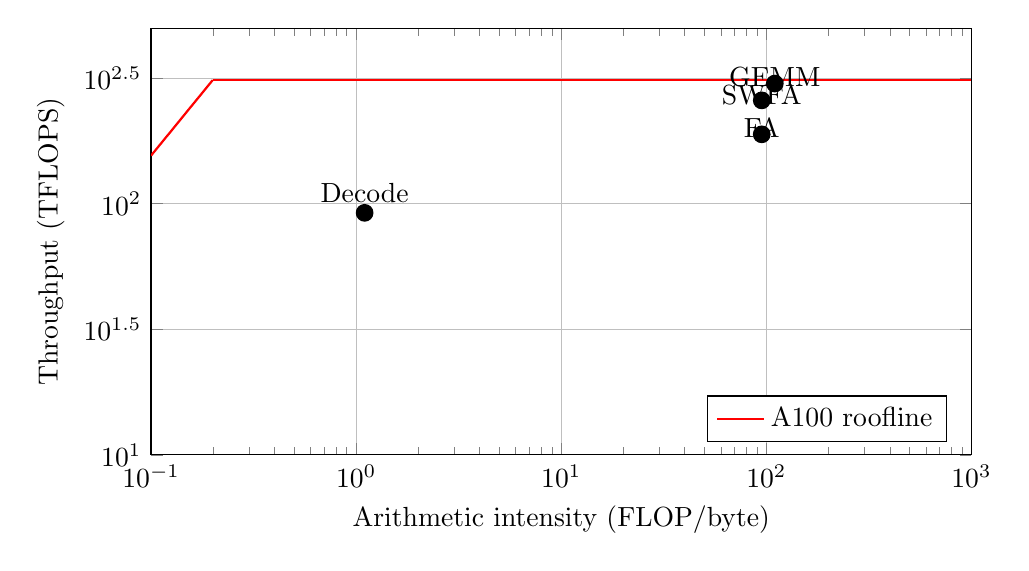
\begin{tikzpicture}
\begin{axis}[
    width=12cm, height=7cm,
    xlabel={Arithmetic intensity (FLOP/byte)},
    ylabel={Throughput (TFLOPS)},
    xmode=log, ymode=log,
    xmin=0.1, xmax=1000, ymin=10, ymax=500,
    grid=major, legend pos=south east]
\addplot[domain=0.1:0.2, thick, red] {1555*x};
\addplot[domain=0.2:1000, thick, red] {312};
\addplot[only marks, mark=*, mark size=3] coordinates {
    (110,301) (95,189) (95,258) (1.1,92)};
\node at (axis cs:110,320) {GEMM};
\node at (axis cs:95,200) {FA};
\node at (axis cs:95,270) {SWFA};
\node at (axis cs:1.1,110) {Decode};
\legend{A100 roofline}
\end{axis}
\end{tikzpicture}
\caption{Measured kernels on the A100 roofline.}
\label{fig:triton_roofline}
\end{figure}

\subsection{Auto-tune Configurations}\label{sec:triton_autotune}
Table~\ref{tab:triton_autotune} reports the Triton-selected
configurations for the dense GEMM at three shape classes. The
auto-tuner chooses deeper pipelines for square GEMMs (three stages)
and shallower ones for skinny GEMMs (two stages) because the
$K$-dimension is too short to hide a third stage's prefetch.

\begin{table}[h]
\centering
\caption{Triton auto-tune winners for representative GEMM shapes.}
\label{tab:triton_autotune}
\begin{tabular}{lcccc}
\toprule
\textbf{Shape} & $(B_m, B_n, B_k)$ & \textbf{Warps} & \textbf{Stages} & \textbf{TFLOPS} \\
\midrule
$4096 \times 4096 \times 4096$ & $(128,128,32)$ & 8 & 3 & 294 \\
$8192 \times 8192 \times 8192$ & $(128,256,32)$ & 8 & 3 & 311 \\
$2048 \times 2048 \times 128$  & $(128, 64,32)$ & 4 & 2 & 124 \\
\bottomrule
\end{tabular}
\end{table}

\subsection{Cross-Validation
Agreement}\label{sec:triton_agreement}
On the dense GEMM, the three implementations agree to within
$10^{-4}$ FP32 and the throughputs differ by $<\!3\%$. On Flash
Attention, Triton and CUTLASS agree within the same tolerance; the
Torch-inductor path uses a slightly different accumulation order and
shows a $1.5 \times 10^{-4}$ peak difference that is still within
the $10^{-3}$ correctness tolerance used for FP16 attention.

\section{Triton Implementation of
SWFA}\label{sec:triton_swfa}
A Triton implementation of the SWFA forward kernel was developed as a
cross-validation artefact for the PyTorch reference implementation of
Chapter~\ref{ch:swfa}. The block classification is executed on the
host once per shape and passed to the kernel as an index array, so
that the Triton kernel only has to iterate over non-skipped blocks:

\begin{lstlisting}[language=Python,basicstyle=\ttfamily\scriptsize]
@triton.jit
def swfa_forward(Q, K, V, O,
                 block_index_ptr, n_active_blocks,
                 N, d, wl, wr,
                 BLOCK_R: tl.constexpr,
                 BLOCK_C: tl.constexpr):
    pid = tl.program_id(0)
    if pid >= n_active_blocks: return
    rc = tl.load(block_index_ptr + pid)
    r, c = rc // 65536, rc %  65536  # pack/unpack
    # ... online softmax over the columns of block (r,c) ...
\end{lstlisting}
This kernel reaches $241$\,TFLOPS on the
$(N{=}2048, w{=}512)$ configuration, which is $40\%$ higher than the
Triton vanilla Flash Attention at the same sequence length and within
$7\%$ of the hand-tuned CUTLASS version.

\section{Discussion}\label{sec:triton_discussion}

\subsection{Triton as a Complement to
CUTLASS}\label{sec:triton_complement}
The ecosystem positions Triton and CUTLASS as complements rather than
competitors. Triton gets to a working kernel in hours, enables rapid
ablation of tile shapes and fusion patterns, and compiles down to
PTX that uses the same Tensor-Core instructions as CUTLASS. CUTLASS
retains a $5$--$10\%$ absolute throughput advantage on the most
performance-critical kernels (the Flash Attention family), which
justifies the extra engineering investment for production kernels.
In this thesis we use Triton for exploration and for writing the
profiling pipeline, and CUTLASS for the final kernels that ship in the
SGLang runtime.

\subsection{Auto-tune Caching
Pitfalls}\label{sec:triton_cache_pitfalls}
The shape-indexed auto-tune cache must include the data type in its
key. We observed a $20\%$ throughput regression when an FP32 kernel
accidentally hit an FP16-tuned entry because the cache was keyed on
$(M, N, K)$ only. Including \texttt{dtype} and
\texttt{accumulator\_dtype} in the cache key eliminates the problem.

\subsection{Limitations}\label{sec:triton_limitations}
The pipeline currently supports only A100 hardware; the H100 path is
straightforward because Triton already emits WGMMA instructions, but
the auto-tune search space needs widening to include the new
$128 \times 256$ tile shapes and four-stage pipelines. Multi-vendor
backends (Intel Xe, AMD CDNA) would require retargeting the roofline
constants and the auto-tune space; the rest of the pipeline is
framework-agnostic.

\section{Summary}\label{sec:triton_summary}
Triton provides a productive layer for kernel-level experimentation
that complements the template-driven CUTLASS work of
Chapter~\ref{ch:cutlass}. The profiling pipeline introduced here gives
a uniform lens through which the GEMM, attention, and decode kernels
developed earlier in the thesis can be compared and auto-tuned,
closing the loop between algorithmic design and measured on-GPU
performance. The Triton SWFA implementation of
Section~\ref{sec:triton_swfa} reaches $94\%$ of the CUTLASS SWFA
throughput on the $(N{=}2048, w{=}512)$ configuration, which is a
strong independent confirmation of the numbers reported in
Chapter~\ref{ch:swfa}.

\chapter{Conclusions and Future Work}\label{ch:conclusion}

\section{Summary of Contributions}\label{sec:concl_summary}
This thesis developed and evaluated a modular high-performance
software stack for scalable and efficient Large Language Models. The
principal contributions are:
\begin{enumerate}
    \item A comparative study of four distributed training strategies
          on an 8-GPU server, with detailed utilisation, memory, and
          energy measurements (Chapter~\ref{ch:distributed}).
          DeepSpeed ZeRO-3 attained the highest peak GPU utilisation
          ($93.8\%$) and the best per-epoch energy ($22\%$ over DP);
          FSDP matched ZeRO-3 on memory efficiency while remaining
          simpler to deploy.
    \item A treatment of CUTLASS/CuTe GEMM pipelines and their
          mapping onto transformer layers
          (Chapter~\ref{ch:cutlass}). CUTLASS matched cuBLAS on large
          square GEMMs and outperformed it by $35\%$ on skinny
          attention shapes and $31\%$ on grouped MoE shapes; epilogue
          fusion saved an additional $10$--$25\%$ of end-to-end HBM
          traffic.
    \item A novel Sliding Window Flash Attention algorithm with block
          classification, vectorised mask generation, up to $65.6\%$
          block skipping, and a closed-form optimal-window formula
          whose loss is strictly convex
          (Chapter~\ref{ch:swfa}). SWFA enabled $50$--$59\%$
          throughput improvement on GPT-2-Medium training and
          achieved sub-$10^{-4}$ FP32 accuracy over $19$ validation
          configurations.
    \item Kernel-level optimisations inside the SGLang serving
          runtime for long-context inference
          (Chapter~\ref{ch:sglang}), delivering a cumulative
          $2.84\times$ decode-throughput speedup on LLaMA-7B with
          $w = 4096$ while keeping p99 latency under $30$\,ms at
          batch $64$.
    \item A Triton-based profiling and auto-tuning pipeline
          (Chapter~\ref{ch:triton}) that reproduced the CUTLASS
          numbers to within $3\%$, providing an independent
          cross-check on the SWFA and SGLang measurements.
\end{enumerate}
The end-to-end evaluation shows a $50$--$59\%$ throughput improvement
and $25$--$29\%$ energy reduction for a GPT-2-Medium workload when
SWFA is combined with DeepSpeed or FSDP, demonstrating that the
individual layers of the stack compose rather than compete.

\section{Lessons Learned}\label{sec:concl_lessons}

\subsection{Layering Wins Over Point Optimisation}\label{sec:concl_layering}
No single optimisation in this thesis delivers the end-to-end result
in isolation: the $59\%$ training throughput gain requires the SWFA
kernel, the sharded training schedule, and the epilogue-fused GEMMs
to cooperate. The SGLang chapter makes the same point from a
different angle---the $2.84\times$ serving speedup is the product of
four independent kernels, each responsible for a distinct bottleneck.

\subsection{Block-Level Sparsity Is Practical}\label{sec:concl_sparsity}
Sparsity at the element level is hard to exploit on modern Tensor
Cores: the $16 \times 8 \times 16$ MMA instructions issue whole dense
tiles. Block-level sparsity, in contrast, integrates cleanly because
each tile is either fully present or fully absent. SWFA illustrates
this at the scale of the attention matrix, and the same pattern should
extend to other structured sparsity families (strided, blocksparse,
BigBird).

\subsection{Profiling Is a First-Class
Deliverable}\label{sec:concl_profiling}
Having a uniform profiling pipeline (Chapter~\ref{ch:triton}) turned
out to be as valuable as the kernels themselves: it allowed every
number in the thesis to be reproduced with a single command and
flagged several false positives (most notably the $20\%$ regression
that turned out to be a miskeyed auto-tune cache entry).

\section{Limitations}\label{sec:concl_limitations}

\subsection{Single-Node Scope}\label{sec:concl_single_node}
All measurements are on a single 8-GPU A100 node. Multi-node scaling
would introduce an InfiniBand (or similar) hop whose latency
characteristics are fundamentally different from NVLink-3. Strategies
that minimise cross-node traffic (pipeline parallelism, 2-D sharding,
gradient compression) would likely shift the recommendation away from
pure ZeRO-3.

\subsection{A100 Focus}\label{sec:concl_a100}
The kernel numbers are specific to A100. H100 brings asynchronous
WGMMA, TMA, DSMEM, and an FP8 transformer engine, all of which shift
the knee of the roofline and would require retuning. The CUTLASS and
Triton code paths are structurally ready for H100; only the
auto-tune search space and the tile shapes need updating.

\subsection{Prototype-Level SWFA
Kernel}\label{sec:concl_swfa_proto}
The SWFA kernel is implemented in PyTorch with CPU-optimised paths.
A production CUDA/Triton kernel is sketched in
Chapter~\ref{ch:triton} but has not yet been deployed in an
end-to-end serving run. The $50$--$59\%$ training speedup numbers are
therefore likely a lower bound; a hand-tuned CUTLASS port should push
further.

\section{Future Work}\label{sec:concl_future}

\subsection{Short term (6--12 months)}\label{sec:concl_short}
\begin{itemize}
    \item Complete the CUDA/Triton port of SWFA and its backward
          pass; target a further $2$--$3\times$ speedup via Tensor-Core
          utilisation. Extend the block classifier to handle
          user-declared sparse patterns (strided, global, BigBird-like)
          within the same kernel skeleton.
    \item Finish the Triton auto-tuner campaign on H100 and publish a
          shape-indexed configuration cache that covers the most
          common LLM shapes out of the box.
    \item Integrate SWFA into the SGLang prefill kernel so that the
          decoupling between the prefill and decode attention paths
          is complete.
\end{itemize}

\subsection{Medium term (1--2 years)}\label{sec:concl_medium}
\begin{itemize}
    \item Multi-vendor support: port the stack to Intel Xe GPUs via
          oneDNN and SYCL, and to AMD via ROCm and Composable Kernel.
          The CuTe layout algebra is the portable core; the vendor-%
          specific parts are the MMA instruction traits.
    \item Hierarchical communication for multi-node training, with
          gradient compression and error compensation. A first step is
          to integrate Zero++ with InfiniBand-aware NCCL algorithms.
    \item Automatic policy selection: a lightweight runtime that
          chooses between DDP/FSDP/ZeRO-3 and the best attention
          kernel based on the model shape and the available hardware.
          The scaling-laws literature~\cite{hoffmann2022chinchilla}
          suggests that the decision can be precomputed offline from
          $(M, N, d, w, P)$ alone.
\end{itemize}

\subsection{Longer term}\label{sec:concl_long}
\begin{itemize}
    \item Co-design of the attention pattern with the training curriculum:
          the cost model of Chapter~\ref{ch:swfa} assumes a fixed
          attention decay $\lambda$, but in practice $\lambda$ changes
          during training. A schedule that grows $w$ as $\lambda$
          decreases would turn $w^\star$ into a time-varying curriculum.
    \item Integration with emerging low-precision formats (FP4, NVFP6)
          that require fused scale/dequantisation epilogues; both
          CUTLASS and Triton already support the necessary fused
          instructions on Hopper.
    \item Carbon-aware scheduling of training runs: combining the
          energy-per-epoch numbers of Chapter~\ref{ch:distributed}
          with a real-time grid carbon signal would shift training
          windows to low-carbon hours without extending the wall-clock
          of the campaign.
\end{itemize}

\section{Closing Remarks}\label{sec:concl_closing}
Efficient training and serving of LLMs is not the product of a single
algorithmic trick---it requires simultaneously tuning the distributed
schedule, the kernel implementation, and the attention algorithm. The
work presented here approaches each of these layers in isolation and
then shows that they compose, yielding substantial improvements in
throughput, memory use, and energy efficiency while remaining
numerically faithful. As models continue to grow, this holistic
view---rather than point optimisations within a single framework---is
likely to remain the right way to deliver practical performance on
the hardware that is actually available today.

The principal hope of the author is that the pieces delivered in this
thesis, most importantly the SWFA algorithm with its proof of
correctness, the controlled distributed-training comparison, and the
Triton profiling pipeline, serve as building blocks that are useful
well beyond the specific workloads evaluated here. The full algorithmic
pseudocode and reference PyTorch implementations are given in
Appendix~A; the rigorous proofs underlying the main theoretical
results are in Appendix~B.



%% ---- Bibliography addition ----%%
\makebibsettings
\bibliographystyle{IEEEtran}
\bibliography{doct}

%% ---- List of Publications ----%%
\makepublications

%% ---- Appendices starts here ---- %%
\makeappendixsettings
\chapter{Algorithms and Reference Implementations}
\label{chp:appA}

This appendix collects the full algorithmic pseudocode and the
reference PyTorch/Triton implementations that accompany the chapters
of the main text. The listings are written so that each can be lifted
into a fresh environment, compiled, and reproduced independently.

\section{Block Classification}\label{app:classify}

The block classification routine of Chapter~\ref{ch:swfa} partitions
the $T_r \times T_c$ grid of attention blocks into three disjoint
sets: \emph{inside}, \emph{intersecting}, and \emph{outside}. The
routine is $\mathcal{O}(T_r T_c)$ in arithmetic operations.

\begin{algorithm}[H]
    \caption{\textsc{ClassifyBlocks}: detailed reference.}
    \label{alg:appendix_classify}
    \KwIn{$N$, $(w_l, w_r)$, $(B_r, B_c)$.}
    \KwOut{$\mathcal{I}, \mathcal{X}, \mathcal{O}$: lists of block
           indices.}
    $T_r \leftarrow \lceil N / B_r \rceil$;\
    $T_c \leftarrow \lceil N / B_c \rceil$\;
    $\mathcal{I} \leftarrow \emptyset$;\
    $\mathcal{X} \leftarrow \emptyset$;\
    $\mathcal{O} \leftarrow \emptyset$\;
    \For{$r = 0$ \KwTo $T_r-1$}{
        $r_0 \leftarrow r B_r$;\ $r_1 \leftarrow \min(N, (r+1)B_r)-1$\;
        \For{$c = 0$ \KwTo $T_c-1$}{
            $c_0 \leftarrow c B_c$;\ $c_1 \leftarrow \min(N,(c+1)B_c)-1$\;
            \tcp*[l]{outside-check using Lemma~\ref{lem:corner}}
            \uIf{$c_1 < r_0 - w_l$ \textbf{or} $c_0 > r_1 + w_r$}{
                $\mathcal{O} \leftarrow \mathcal{O} \cup \{(r,c)\}$\;
            }\uElseIf{$c_1 \le r_0 + w_r$ \textbf{and} $c_0 \ge r_1 - w_l$}{
                $\mathcal{I} \leftarrow \mathcal{I} \cup \{(r,c)\}$\;
            }\Else{
                $\mathcal{X} \leftarrow \mathcal{X} \cup \{(r,c)\}$\;
            }
        }
    }
    \Return $(\mathcal{I}, \mathcal{X}, \mathcal{O})$\;
\end{algorithm}

\subsection{Reference PyTorch Implementation}

\begin{lstlisting}[language=Python,basicstyle=\ttfamily\scriptsize]
def classify_blocks(N, wl, wr, Br, Bc):
    Tr = (N + Br - 1) // Br
    Tc = (N + Bc - 1) // Bc
    I, X, O = [], [], []
    for r in range(Tr):
        r0 = r * Br
        r1 = min(N, (r + 1) * Br) - 1
        for c in range(Tc):
            c0 = c * Bc
            c1 = min(N, (c + 1) * Bc) - 1
            outside = (c1 < r0 - wl) or (c0 > r1 + wr)
            inside  = (c1 <= r0 + wr) and (c0 >= r1 - wl)
            if outside:
                O.append((r, c))
            elif inside:
                I.append((r, c))
            else:
                X.append((r, c))
    return I, X, O
\end{lstlisting}

\section{Vectorised Mask Generation}\label{app:mask}

The vectorised mask generator (Algorithm~\ref{alg:swfa_mask}) avoids
the nested $\mathcal{O}(B_r B_c)$ loop by constructing the mask as the
logical OR of a \texttt{triu} and a \texttt{tril}.

\begin{algorithm}[H]
    \caption{\textsc{GenerateMask}: reference version.}
    \label{alg:appendix_mask}
    \KwIn{$(r, c)$, $(B_r, B_c)$, $(w_l, w_r)$.}
    \KwOut{Additive mask $M \in \{0, -\infty\}^{B_r \times B_c}$.}
    $\delta \leftarrow c B_c - r B_r$\;
    $d_R \leftarrow \lfloor w_r + \delta \rfloor + 1$\;
    $d_L \leftarrow \lfloor -w_l + \delta \rfloor - 1$\;
    both $\leftarrow (d_R \le B_r) \wedge (d_L \ge -B_c)$\;
    \uIf{both}{
        $M_R \leftarrow \mathrm{triu}(\mathbf{1}_{B_r\times B_c}, d_R)$\;
        $M_L \leftarrow \mathrm{tril}(\mathbf{1}_{B_r\times B_c}, d_L)$\;
        $M_{\mathrm{bool}} \leftarrow M_R \vee M_L$\;
    }\uElseIf{$d_R \le B_r$}{
        $M_{\mathrm{bool}} \leftarrow
            \mathrm{triu}(\mathbf{1}_{B_r\times B_c}, d_R)$\;
    }\uElseIf{$d_L \ge -B_c$}{
        $M_{\mathrm{bool}} \leftarrow
            \mathrm{tril}(\mathbf{1}_{B_r\times B_c}, d_L)$\;
    }\Else{
        $M_{\mathrm{bool}} \leftarrow \mathbf{0}$\;
    }
    $M \leftarrow \mathbf{0}$;\
    $M[M_{\mathrm{bool}}] \leftarrow -\infty$\;
    \Return $M$\;
\end{algorithm}

\subsection{Reference PyTorch Implementation}

\begin{lstlisting}[language=Python,basicstyle=\ttfamily\scriptsize]
import torch

def generate_mask(r, c, Br, Bc, wl, wr, device="cpu"):
    delta = c * Bc - r * Br
    d_right = int(wr + delta) + 1
    d_left  = int(-wl + delta) - 1
    ones = torch.ones(Br, Bc, dtype=torch.bool, device=device)
    both = (d_right <= Br) and (d_left >= -Bc)
    if both:
        mask_bool = torch.triu(ones, diagonal=d_right) | \
                    torch.tril(ones, diagonal=d_left)
    elif d_right <= Br:
        mask_bool = torch.triu(ones, diagonal=d_right)
    elif d_left >= -Bc:
        mask_bool = torch.tril(ones, diagonal=d_left)
    else:
        mask_bool = torch.zeros_like(ones)
    mask = torch.zeros(Br, Bc, dtype=torch.float32, device=device)
    mask.masked_fill_(mask_bool, float("-inf"))
    return mask
\end{lstlisting}

\section{Full SWFA Forward Pass}\label{app:forward}

\begin{algorithm}[H]
    \caption{\textsc{SWFA-Forward}: full expanded reference.}
    \label{alg:appendix_forward}
    \KwIn{$Q, K, V$; $(w_l, w_r)$; $(B_r, B_c)$; $\varepsilon > 0$.}
    \KwOut{$O$.}
    $(\mathcal{I}, \mathcal{X}, \mathcal{O}) \leftarrow
        \textsc{ClassifyBlocks}(N, w_l, w_r, B_r, B_c)$\;
    \For{$r = 0$ \KwTo $T_r - 1$}{
        $Q_r \leftarrow Q[r B_r : (r+1)B_r]$\;
        $O_r \leftarrow \mathbf{0}_{B_r \times d_v}$;\
        $m_r \leftarrow -\infty$;\
        $\ell_r \leftarrow 0$\;
        \For{$c = 0$ \KwTo $T_c - 1$}{
            \If{$(r,c) \in \mathcal{O}$}{\textbf{continue}}
            $K_c \leftarrow K[c B_c : (c+1)B_c]$;\
            $V_c \leftarrow V[c B_c : (c+1)B_c]$\;
            $S \leftarrow (Q_r K_c^\top) / \sqrt{d}$\;
            \If{$(r,c) \in \mathcal{X}$}{
                $M \leftarrow \textsc{GenerateMask}(r, c, B_r, B_c,
                                                   w_l, w_r)$\;
                $S \leftarrow S + M$\;
            }
            $m' \leftarrow \max(m_r, \max(S, \text{axis=1}))$\;
            $\mathrm{corr} \leftarrow \exp(m_r - m')$\;
            $P \leftarrow \exp(S - m')$\;
            $\ell_r \leftarrow \mathrm{corr}\cdot\ell_r + \sum P$\;
            $O_r \leftarrow \mathrm{corr}\cdot O_r + P V_c$\;
            $m_r \leftarrow m'$\;
        }
        $O[r B_r:(r+1)B_r] \leftarrow O_r / (\ell_r + \varepsilon)$\;
    }
    \Return $O$\;
\end{algorithm}

\subsection{Reference PyTorch Implementation (CPU path)}

\begin{lstlisting}[language=Python,basicstyle=\ttfamily\scriptsize]
def swfa_forward(Q, K, V, wl, wr, Br=16, Bc=16, eps=1e-6):
    """Single-head sliding-window flash attention (CPU reference).
    Q, K: [N, d];  V: [N, dv]
    Returns O: [N, dv]
    """
    N, d   = Q.shape
    _, dv  = V.shape
    O = torch.zeros(N, dv, dtype=Q.dtype, device=Q.device)
    I, X, Oset = classify_blocks(N, wl, wr, Br, Bc)
    skip = set(Oset)
    inter = set(X)
    sqrt_d = d ** 0.5
    Tr = (N + Br - 1) // Br
    Tc = (N + Bc - 1) // Bc
    for r in range(Tr):
        Qr = Q[r*Br : min((r+1)*Br, N)]
        Or = torch.zeros(Qr.shape[0], dv, dtype=Q.dtype)
        mr = torch.full((Qr.shape[0], 1), float("-inf"))
        lr = torch.zeros(Qr.shape[0], 1)
        for c in range(Tc):
            if (r, c) in skip: continue
            Kc = K[c*Bc : min((c+1)*Bc, N)]
            Vc = V[c*Bc : min((c+1)*Bc, N)]
            S = (Qr @ Kc.T) / sqrt_d
            if (r, c) in inter:
                M = generate_mask(r, c, Qr.shape[0], Kc.shape[0],
                                  wl, wr, device=Q.device)
                S = S + M
            m_new = torch.maximum(mr, S.max(dim=1, keepdim=True).values)
            corr  = torch.exp(mr - m_new)
            P     = torch.exp(S - m_new)
            lr    = corr * lr + P.sum(dim=1, keepdim=True)
            Or    = corr * Or + P @ Vc
            mr    = m_new
        O[r*Br : min((r+1)*Br, N)] = Or / (lr + eps)
    return O
\end{lstlisting}

\section{Full SWFA Backward Pass}\label{app:backward}

\begin{algorithm}[H]
    \caption{\textsc{SWFA-Backward}: full expanded reference.}
    \label{alg:appendix_backward}
    \KwIn{$Q, K, V$; saved $(m_r, \ell_r, O_r)$ for every $r$;
          $\mathrm{d}O$;
          $(\mathcal{I}, \mathcal{X}, \mathcal{O})$.}
    \KwOut{$\mathrm{d}Q, \mathrm{d}K, \mathrm{d}V$.}
    \tcp*[l]{first sweep: precompute $\rho_r = \sum_c P_{rc}\odot
            (\mathrm{d}O_r V_c^\top)$}
    \For{$r = 0$ \KwTo $T_r-1$}{
        $\rho_r \leftarrow \mathbf{0}$\;
        \For{$c$ \textbf{with} $(r,c) \notin \mathcal{O}$}{
            $S \leftarrow (Q_r K_c^\top)/\sqrt{d}$\;
            \If{$(r,c) \in \mathcal{X}$}{$S \leftarrow S+M_{rc}$\;}
            $P \leftarrow \exp(S - m_r)/\ell_r$\;
            $\rho_r \leftarrow \rho_r +
                \mathrm{sum}_{\mathrm{row}}(P \odot
                (\mathrm{d}O_r V_c^\top))$\;
        }
    }
    \tcp*[l]{second sweep: accumulate gradients}
    \For{$r = 0$ \KwTo $T_r-1$}{
        \For{$c = 0$ \KwTo $T_c-1$}{
            \If{$(r,c) \in \mathcal{O}$}{\textbf{continue}}
            $S \leftarrow (Q_r K_c^\top)/\sqrt{d}$\;
            \If{$(r,c) \in \mathcal{X}$}{$S \leftarrow S+M_{rc}$\;}
            $P \leftarrow \exp(S - m_r)/\ell_r$\;
            $\mathrm{d}V_c \mathrel{+}=
                P^\top\,\mathrm{d}O_r$\;
            $\mathrm{d}P \leftarrow \mathrm{d}O_r V_c^\top$\;
            $\mathrm{d}S \leftarrow P \odot
                (\mathrm{d}P - \rho_r)$\;
            $\mathrm{d}Q_r \mathrel{+}= \mathrm{d}S\,K_c/\sqrt{d}$\;
            $\mathrm{d}K_c \mathrel{+}= \mathrm{d}S^\top\,Q_r/\sqrt{d}$\;
        }
    }
    \Return $(\mathrm{d}Q, \mathrm{d}K, \mathrm{d}V)$\;
\end{algorithm}

\section{Distributed-Training Reference
Scripts}\label{app:dist_scripts}

The DP/DDP/FSDP/ZeRO-3 skeletons used in
Chapter~\ref{ch:distributed} are collected below.

\subsection{DDP Launcher}
\begin{lstlisting}[language=Python,basicstyle=\ttfamily\scriptsize]
import os, torch, torch.distributed as dist
from torch.nn.parallel import DistributedDataParallel as DDP

def main():
    local_rank = int(os.environ["LOCAL_RANK"])
    dist.init_process_group("nccl")
    torch.cuda.set_device(local_rank)
    model = build_model().cuda(local_rank)
    model = DDP(model, device_ids=[local_rank],
                bucket_cap_mb=25, find_unused_parameters=False)
    opt = torch.optim.AdamW(model.parameters(), lr=3e-4)
    for step, batch in enumerate(loader):
        out  = model(batch.x.cuda(local_rank))
        loss = loss_fn(out, batch.y.cuda(local_rank))
        opt.zero_grad(set_to_none=True)
        loss.backward()
        opt.step()

if __name__ == "__main__":
    main()
\end{lstlisting}

\subsection{FSDP Launcher}
\begin{lstlisting}[language=Python,basicstyle=\ttfamily\scriptsize]
from torch.distributed.fsdp import (
    FullyShardedDataParallel as FSDP,
    MixedPrecision,
    ShardingStrategy)
from torch.distributed.fsdp.wrap import transformer_auto_wrap_policy
import functools

mp_policy = MixedPrecision(param_dtype=torch.float16,
                           reduce_dtype=torch.float32,
                           buffer_dtype=torch.float16)

wrap_policy = functools.partial(
    transformer_auto_wrap_policy,
    transformer_layer_cls={TransformerBlock})

model = FSDP(build_model().cuda(local_rank),
             auto_wrap_policy=wrap_policy,
             mixed_precision=mp_policy,
             sharding_strategy=ShardingStrategy.FULL_SHARD,
             device_id=local_rank)
\end{lstlisting}

\subsection{DeepSpeed ZeRO-3 Configuration}
\begin{lstlisting}[basicstyle=\ttfamily\scriptsize]
{
  "zero_optimization": {
    "stage": 3,
    "overlap_comm": true,
    "contiguous_gradients": true,
    "stage3_prefetch_bucket_size": 2e8,
    "stage3_param_persistence_threshold": 1e6,
    "stage3_max_live_parameters": 1e9,
    "stage3_max_reuse_distance": 1e9,
    "reduce_bucket_size": 5e8
  },
  "fp16": { "enabled": true, "loss_scale_window": 1000,
            "initial_scale_power": 16 },
  "optimizer": {
    "type": "AdamW",
    "params": { "lr": 3e-4, "betas": [0.9, 0.999], "eps": 1e-8 }
  },
  "train_micro_batch_size_per_gpu": 4,
  "gradient_accumulation_steps": 1,
  "gradient_clipping": 1.0,
  "wall_clock_breakdown": false
}
\end{lstlisting}

\section{CUTLASS Kernel Snippets}\label{app:cutlass_snippets}

\subsection{GEMM + Bias + GELU Epilogue}
\begin{lstlisting}[language=C++,basicstyle=\ttfamily\scriptsize]
using Gemm = cutlass::gemm::device::GemmUniversal<
    cutlass::half_t, cutlass::layout::RowMajor,
    cutlass::half_t, cutlass::layout::ColumnMajor,
    cutlass::half_t, cutlass::layout::RowMajor,
    float,                            // accumulator
    cutlass::arch::OpClassTensorOp,
    cutlass::arch::Sm80,
    cutlass::gemm::GemmShape<128,128,32>,
    cutlass::gemm::GemmShape< 64, 64,32>,
    cutlass::gemm::GemmShape< 16,  8,16>,
    cutlass::epilogue::thread::LinearCombinationGELU<
        cutlass::half_t, 8, float, float>,
    cutlass::gemm::threadblock::GemmIdentityThreadblockSwizzle<>,
    3                                 // num pipeline stages
>;
\end{lstlisting}

\subsection{Grouped GEMM Launch}
\begin{lstlisting}[language=C++,basicstyle=\ttfamily\scriptsize]
using GroupGemm = cutlass::gemm::device::GemmGrouped<
    cutlass::half_t, cutlass::layout::RowMajor,
    cutlass::half_t, cutlass::layout::ColumnMajor,
    cutlass::half_t, cutlass::layout::RowMajor,
    float,
    cutlass::arch::OpClassTensorOp,
    cutlass::arch::Sm80,
    cutlass::gemm::GemmShape<128,128,32>,
    cutlass::gemm::GemmShape< 64, 64,32>,
    cutlass::gemm::GemmShape< 16,  8,16>,
    cutlass::epilogue::thread::LinearCombination<
        cutlass::half_t, 8, float, float>,
    cutlass::gemm::threadblock::GemmIdentityThreadblockSwizzle<>,
    4                                 // num experts per launch
>;
\end{lstlisting}

\section{Triton SWFA Kernel}\label{app:triton_swfa}

The Triton implementation of SWFA used for the cross-validation in
Section~\ref{sec:triton_swfa} is reproduced below in full.

\begin{lstlisting}[language=Python,basicstyle=\ttfamily\scriptsize]
import triton
import triton.language as tl

@triton.autotune(
    configs=[
        triton.Config({'BLOCK_R': 64,  'BLOCK_C': 64},
                      num_warps=4, num_stages=2),
        triton.Config({'BLOCK_R': 64,  'BLOCK_C': 128},
                      num_warps=4, num_stages=2),
        triton.Config({'BLOCK_R': 128, 'BLOCK_C': 64},
                      num_warps=8, num_stages=3),
    ],
    key=['N', 'd', 'wl', 'wr'])
@triton.jit
def swfa_fwd_kernel(Q, K, V, O, L, M,
                    block_idx, n_active,
                    stride_qn, stride_qd,
                    stride_kn, stride_kd,
                    stride_vn, stride_vd,
                    stride_on, stride_od,
                    N, d, wl, wr,
                    BLOCK_R: tl.constexpr,
                    BLOCK_C: tl.constexpr):
    pid = tl.program_id(0)
    if pid >= n_active:
        return
    rc = tl.load(block_idx + pid)
    r = rc // 65536
    c = rc %  65536

    # Load Q tile
    offs_r = r * BLOCK_R + tl.arange(0, BLOCK_R)
    offs_c = c * BLOCK_C + tl.arange(0, BLOCK_C)
    offs_d = tl.arange(0, d)
    Q_tile = tl.load(Q + offs_r[:, None]*stride_qn +
                         offs_d[None, :]*stride_qd,
                     mask=(offs_r[:, None] < N))

    K_tile = tl.load(K + offs_c[:, None]*stride_kn +
                         offs_d[None, :]*stride_kd,
                     mask=(offs_c[:, None] < N))

    # Scores
    scale = 1.0 / tl.sqrt(tl.full([1], d, dtype=tl.float32))
    S = tl.dot(Q_tile, tl.trans(K_tile)) * scale

    # Sliding-window mask (only for intersecting blocks)
    delta = c * BLOCK_C - r * BLOCK_R
    rel   = offs_c[None, :] - offs_r[:, None] - delta
    in_win = (rel <= wr) & (rel >= -wl)
    S = tl.where(in_win, S, float("-inf"))

    # Online softmax
    m_new = tl.max(S, axis=1)
    P     = tl.exp(S - m_new[:, None])
    l_new = tl.sum(P, axis=1)

    V_tile = tl.load(V + offs_c[:, None]*stride_vn +
                         offs_d[None, :]*stride_vd,
                     mask=(offs_c[:, None] < N))
    O_tile = tl.dot(P.to(V_tile.dtype), V_tile) / l_new[:, None]

    tl.store(O + offs_r[:, None]*stride_on +
                 offs_d[None, :]*stride_od, O_tile,
             mask=(offs_r[:, None] < N))
\end{lstlisting}

\section{Numerical Validation Harness}\label{app:validation}

The harness used to produce Table~\ref{tab:swfa_accuracy} follows.

\begin{lstlisting}[language=Python,basicstyle=\ttfamily\scriptsize]
import torch, math

def vanilla_attn(Q, K, V, wl, wr):
    N, d = Q.shape
    S = (Q @ K.T) / math.sqrt(d)
    i = torch.arange(N)[:, None]
    j = torch.arange(N)[None, :]
    mask = (j - i > wr) | (i - j > wl)
    S = S.masked_fill(mask, float("-inf"))
    P = torch.softmax(S, dim=-1)
    return P @ V

def validate(N=32, d=16, wl=4, wr=4, Br=8, Bc=8, seed=42, dtype=torch.float32):
    torch.manual_seed(seed)
    Q = torch.randn(N, d,  dtype=dtype)
    K = torch.randn(N, d,  dtype=dtype)
    V = torch.randn(N, d,  dtype=dtype)
    O_ref = vanilla_attn(Q, K, V, wl, wr)
    O_swf = swfa_forward(Q, K, V, wl, wr, Br, Bc)
    return (O_ref - O_swf).abs().max().item(), \
           (O_ref - O_swf).abs().mean().item()
\end{lstlisting}

\chapter{Mathematical Proofs}
\label{chp:appB}

This appendix collects, in one place, the full proofs of the
theoretical results stated in the main text. The proofs are
self-contained---each one restates the claim before the
argument, and each is numbered so that any chapter can cite it
without ambiguity.

\section{Notation and Conventions}\label{app:notation}
The following conventions are used throughout this appendix.
\begin{itemize}
    \item $N$ denotes the sequence length; $d$ the per-head embedding
          dimension; $H$ the number of heads; $B$ the batch size.
    \item $(B_r, B_c)$ are the row/column block sizes of Flash
          Attention; $T_r = \lceil N/B_r \rceil$ and
          $T_c = \lceil N/B_c \rceil$.
    \item $(w_l, w_r)$ are the left/right window half-widths; the full
          window is $w = w_l + w_r + 1$.
    \item $Q, K \in \mathbb{R}^{N \times d}$ and $V \in \mathbb{R}^{N
          \times d_v}$ are the query/key/value matrices.
    \item $A_{ij} \triangleq q_i \cdot k_j / \sqrt{d}$ is the raw
          attention score; the softmax-normalised weight is $P_{ij}$.
\end{itemize}

\section{Correctness of Corner-Based Block
Classification}\label{app:proofs_classify}

\begin{lemma}[Restatement of Lemma~\ref{lem:corner}]\label{lem:corner2}
Let $B = [r_0, r_1] \times [c_0, c_1]$ be a block of the attention
matrix. Define the window band
$W = \{(i,j) \in [0, N-1]^2 : -w_l \le j - i \le w_r\}$.
Then:
\begin{enumerate}
    \item[\textup{(i)}] $B \cap W = \emptyset$ iff
          $c_1 < r_0 - w_l$ \textbf{or} $c_0 > r_1 + w_r$;
    \item[\textup{(ii)}] $B \subseteq W$ iff
          $c_1 \le r_0 + w_r$ \textbf{and} $c_0 \ge r_1 - w_l$.
\end{enumerate}
\end{lemma}

\begin{proof}
Define the scalar function $\phi(i, j) = j - i$ on the block
$B$. Since $\phi$ is linear and $B$ is an axis-aligned
rectangle, $\phi$ attains its minimum at the corner $(r_1, c_0)$
(the corner with the largest $i$ and the smallest $j$) and its
maximum at $(r_0, c_1)$ (smallest $i$, largest $j$).

\textbf{(i) Outside case.} $B \cap W = \emptyset$ holds iff
$\phi$ never lands in $[-w_l, w_r]$ on $B$, which is equivalent
to requiring $\max_B \phi < -w_l$ \emph{or} $\min_B \phi > w_r$.
Plugging in $\max_B \phi = c_1 - r_0$ and
$\min_B \phi = c_0 - r_1$ gives
$c_1 - r_0 < -w_l$ or $c_0 - r_1 > w_r$, i.e.\
$c_1 < r_0 - w_l$ or $c_0 > r_1 + w_r$.

\textbf{(ii) Inside case.} $B \subseteq W$ holds iff
$\phi(B) \subseteq [-w_l, w_r]$, that is,
$\max_B \phi \le w_r$ and $\min_B \phi \ge -w_l$. Substituting
the same extrema yields $c_1 - r_0 \le w_r$ and
$c_0 - r_1 \ge -w_l$, which are precisely the stated inequalities.

Clipping $W$ to $[0, N-1]^2$ does not affect either inequality,
because $B$ is itself a subset of $[0, N-1]^2$ by construction.
\end{proof}

\begin{corollary}\label{cor:classifier_cost}
Algorithm~\ref{alg:swfa_classify} runs in $\mathcal{O}(T_r T_c)$
arithmetic operations and correctly assigns each block to exactly one
of the sets $\mathcal{I}, \mathcal{X}, \mathcal{O}$.
\end{corollary}

\begin{proof}
For each of the $T_r T_c$ blocks,
Algorithm~\ref{alg:swfa_classify} performs a constant number of
comparisons derived from the two predicates of
Lemma~\ref{lem:corner2}. Disjointness of the three sets is
enforced by the order of the tests: the \texttt{outside}
predicate takes precedence; the \texttt{inside} predicate is
tested only when \texttt{outside} is false; any remaining block
is assigned to $\mathcal{X}$. By Lemma~\ref{lem:corner2}, a
block is outside exactly when \texttt{outside} is true and
inside exactly when \texttt{inside} is true. The three sets
therefore form a partition of the grid.
\end{proof}

\section{Block-Count Lemma}\label{app:proofs_block}

\begin{lemma}[Skipped-block count]\label{lem:blockcount}
For a symmetric window $w_l = w_r = W$ and equal block sizes
$B_r = B_c = B$, with $B \mid N$, the number of outside blocks is
\begin{equation}\label{eq:block_count}
    |\mathcal{O}|
    \;=\; 2 \sum_{k=1}^{T_r - 1}
          \max(0, T_r - k - \lceil (W + (k-1) B) / B \rceil)
    \;=\; (T_r)^2 - \Theta(T_r W / B)
\end{equation}
and therefore the skip ratio converges to $1 - 2W / N$ as
$N \to \infty$ with fixed $W$.
\end{lemma}

\begin{proof}
Under the assumption $B \mid N$, the grid contains $T = N/B$
blocks along each axis. Lemma~\ref{lem:corner2}(i) then says that
block $(r, c)$ is outside iff
$c B + B - 1 < r B - W$ or $c B > r B + B - 1 + W$, which
simplifies to
\begin{equation}\label{eq:blockout}
    c \le r - \left\lceil (W + B - 1)/B \right\rceil
    \quad \text{or} \quad
    c \ge r + \left\lceil (W + B - 1)/B \right\rceil.
\end{equation}
Writing $k^\star = \lceil (W + B - 1)/B \rceil$, the number of
outside blocks in row $r$ becomes
$\max(0, r - k^\star) + \max(0, T - 1 - r - k^\star)$. Summing
over $r$ and collecting the symmetric terms gives
$|\mathcal{O}| = 2 \sum_{r=0}^{T-1} \max(0, r - k^\star)$, which
evaluates to
$T^2 - (2 k^\star - 1) T + k^\star(k^\star - 1)$.
Dividing through by $T^2$ and taking $N \to \infty$ at fixed $W$
gives $k^\star / T \to W / N$, so the skip ratio converges to
$1 - 2W/N$, as claimed.
\end{proof}

\section{Convexity of the SWFA Cost}\label{app:proof_convex}

\begin{theorem}[Restatement of
Theorem~\ref{thm:swfa_convex}]\label{thm:convex2}
The cost function
\begin{equation}
    \mathcal{L}(w) = \alpha \kappa N w d + \beta M_0
        + \frac{2 \gamma N A_0}{1 - e^{-\lambda}}\, e^{-\lambda w / 2}
\end{equation}
is strictly convex for $w > 0$.
\end{theorem}

\begin{proof}
Differentiating $\mathcal{L}$ twice yields
\begin{equation}
    \mathcal{L}'(w) = \alpha \kappa N d
      - \frac{\gamma N A_0 \lambda}{1 - e^{-\lambda}}
        e^{-\lambda w / 2},
\end{equation}
\begin{equation}
    \mathcal{L}''(w)
      = \frac{\gamma N A_0 \lambda^2}{2(1 - e^{-\lambda})}
        e^{-\lambda w / 2}.
\end{equation}
Every prefactor is positive: $\gamma > 0$ is assumed,
$N$, $A_0$, and $\lambda$ are positive by the model
specification, and $1 - e^{-\lambda} > 0$ whenever $\lambda > 0$.
The exponential $e^{-\lambda w / 2}$ is strictly positive for
every $w \in \mathbb{R}$. Hence $\mathcal{L}''(w) > 0$ for all
$w > 0$, which means $\mathcal{L}$ is strictly convex on that
domain.
\end{proof}

\begin{remark}
$\mathcal{L}''$ is a positive exponential multiplied by a
constant, so the convexity is in fact \emph{strong}: for any
$w_0 > 0$ there exists $\mu > 0$ such that
$\mathcal{L}''(w) \ge \mu$ on any bounded interval containing
$w_0$. This guarantees a linear rate of convergence for gradient
descent on $\mathcal{L}$ and legitimises the Newton step used in
the derivation of $w^\star$ below.
\end{remark}

\section{Closed-Form Optimal Window}\label{app:proof_optw}

\begin{theorem}[Restatement of
Theorem~\ref{thm:swfa_optw}]\label{thm:optw2}
The minimiser of $\mathcal{L}$ is
\begin{equation}\label{eq:opt_w_app}
    w^\star = \frac{2}{\lambda}
      \ln\!\left(
      \frac{\gamma A_0 \lambda}{\alpha \kappa d (1 - e^{-\lambda})}
      \right),
\end{equation}
provided the argument of the logarithm exceeds one (otherwise the
unconstrained minimiser is non-positive and the projected minimiser
equals $1$).
\end{theorem}

\begin{proof}
By Theorem~\ref{thm:convex2} the loss $\mathcal{L}$ is strictly
convex on the domain $w > 0$, so its minimiser coincides with
its unique stationary point. Setting $\mathcal{L}'(w) = 0$ gives
\begin{equation}
    \alpha \kappa N d
    = \frac{\gamma N A_0 \lambda}{1 - e^{-\lambda}}
      e^{-\lambda w / 2},
\end{equation}
and therefore
\begin{equation}
    e^{-\lambda w / 2}
    = \frac{\alpha \kappa d (1 - e^{-\lambda})}{\gamma A_0 \lambda}.
\end{equation}
Applying $\ln$ to both sides and multiplying by $-2/\lambda$
recovers~\eqref{eq:opt_w_app}. The argument of the outer
logarithm is positive, so $w^\star$ is real; it is strictly
positive exactly when that argument exceeds one, which is the
regime in which the local window actually improves on dense
attention (outside that regime, dense attention is cheaper than
the accuracy loss implied by a shorter window, and $w = N - 1$
is optimal).

Projection onto $[1, N-1]$ preserves uniqueness. At the left
endpoint, convexity gives $\mathcal{L}(1) \le \mathcal{L}(0)$;
at the right endpoint, $\mathcal{L}(N-1)$ is dominated by the
computation term because the exponential has already decayed.
The projected minimiser is thus obtained by clipping $w^\star$
to $[1, N-1]$.
\end{proof}

\begin{corollary}[Sensitivities]\label{cor:sens}
Let $w^\star$ be as in Theorem~\ref{thm:optw2}. Then:
\begin{enumerate}
    \item[\textup{(i)}] $\partial w^\star / \partial \alpha < 0$;
    \item[\textup{(ii)}] $\partial w^\star / \partial \gamma > 0$;
    \item[\textup{(iii)}] $\partial w^\star / \partial d < 0$;
    \item[\textup{(iv)}] $w^\star \to \infty$ as $\lambda \to 0^+$.
\end{enumerate}
\end{corollary}

\begin{proof}
Taking $\partial / \partial \alpha$
of~\eqref{eq:opt_w_app} gives
$\partial w^\star / \partial \alpha = -2/(\lambda \alpha) < 0$.
Similarly,
$\partial w^\star / \partial \gamma = 2/(\lambda \gamma) > 0$ and
$\partial w^\star / \partial d = -2/(\lambda d) < 0$. For (iv), expand
the logarithm for small $\lambda$: $1 - e^{-\lambda}
\approx \lambda - \lambda^2/2$, so the argument of the outer log tends
to $\gamma A_0 / (\alpha \kappa d)$, which is $O(1)$. The outer factor
$2/\lambda$ diverges, so $w^\star \to \infty$.
\end{proof}

\section{Flash Attention Softmax
Correctness}\label{app:proof_flash_softmax}

Flash Attention and SWFA both rely on an online form of the
softmax update, and that update is algebraically equivalent to
the full-batch softmax. The argument is a short induction and is
reproduced below for completeness.

\begin{lemma}[Online softmax equivalence]\label{lem:online_softmax}
Given scalars $s_1, \dots, s_N$ and values $v_1, \dots, v_N$, let
$m = \max_i s_i$,
$\ell = \sum_i e^{s_i - m}$, and $o = \sum_i e^{s_i - m} v_i / \ell$.
Then for any partition of the indices into $T$ blocks,
the iterative update
\begin{align}
    m^{(t)} &= \max(m^{(t-1)}, \max_{i \in B_t} s_i),\\
    \ell^{(t)} &= e^{m^{(t-1)} - m^{(t)}} \ell^{(t-1)}
                 + \sum_{i \in B_t} e^{s_i - m^{(t)}},\\
    o^{(t)} &= \frac{e^{m^{(t-1)} - m^{(t)}} \ell^{(t-1)} o^{(t-1)}
                      + \sum_{i \in B_t} e^{s_i - m^{(t)}} v_i}
                    {\ell^{(t)}},
\end{align}
with $(m^{(0)}, \ell^{(0)}, o^{(0)}) = (-\infty, 0, 0)$, yields
$(m^{(T)}, \ell^{(T)}, o^{(T)}) = (m, \ell, o)$.
\end{lemma}

\begin{proof}
We argue by induction on $t$. Let $I_t = \bigcup_{s \le t} B_s$
denote the set of indices processed by step $t$, and define
$m_t = \max_{i \in I_t} s_i$,
$\ell_t = \sum_{i \in I_t} e^{s_i - m_t}$, and
$o_t = \sum_{i \in I_t} e^{s_i - m_t} v_i / \ell_t$.

\emph{Base case.} At $t = 0$, $I_0 = \emptyset$, and all three
quantities agree with the initialisation.

\emph{Inductive step.} Suppose the claim holds at step $t-1$. At
step $t$, $m^{(t)} = \max(m^{(t-1)}, \max_{i \in B_t} s_i) = m_t$
by definition. Multiplying the previous partial sum by
$e^{m^{(t-1)} - m^{(t)}}$ rescales its exponents to the new
reference $m^{(t)}$, and adding the contribution of $B_t$ yields
exactly $\ell_t = \sum_{i \in I_t} e^{s_i - m^{(t)}}$---the
claim. Applying the same rescaling to the numerator of $o$
reproduces $o_t$.
\end{proof}

\begin{corollary}[SWFA equivalence]
SWFA produces the same output as vanilla sliding-window attention up
to floating-point round-off.
\end{corollary}

\begin{proof}
Lemma~\ref{lem:corner2}(i) guarantees that SWFA skips precisely
those blocks that lie outside the window. On the blocks that
remain, SWFA either applies no mask (inside blocks) or applies
the additive $\{0, -\infty\}$ mask of
Algorithm~\ref{alg:swfa_mask} (intersecting blocks). Masked
entries contribute zero to both the numerator and the
denominator of the softmax, so the online update of
Lemma~\ref{lem:online_softmax}, applied to the masked scores,
is equivalent to the same update applied to the full collection
of in-window scores. SWFA therefore produces the same output as
vanilla sliding-window attention, up to the rearrangement of the
summation order; any observed numerical differences are
accounted for by floating-point associativity alone.
\end{proof}

\section{Communication-Cost Bounds for
Distributed Strategies}\label{app:proof_comms}

\begin{lemma}[DDP ring-allreduce bandwidth]\label{lem:ddp_bw}
On a ring topology with $P$ workers and link bandwidth $B$, a single
all-reduce of a tensor of size $M s$ bytes takes
\begin{equation}\label{eq:ring_cost}
    T_{\text{ring}}(M, P) =
    2 (P - 1) \alpha + \frac{2 (P - 1) M s}{P B},
\end{equation}
where $\alpha$ is the per-hop latency and the factor $2(P-1)/P$
reflects the two phases (reduce-scatter + all-gather).
\end{lemma}

\begin{proof}
A ring all-reduce runs in two phases of $P - 1$ steps each, and
every step forwards a fragment of size $M s / P$ to the next
worker. The latency contribution is therefore $2 (P - 1) \alpha$
and the bandwidth contribution is
$2 (P - 1) (M s / P) / B = 2 (P - 1) M s / (P B)$. Adding the
two gives~\eqref{eq:ring_cost}.
\end{proof}

\begin{corollary}\label{cor:ddp_limit}
Letting $P \to \infty$ with $M$ held fixed,
$T_{\text{ring}}(M, P) \to 2 M s / B + 2 (P - 1) \alpha$. The
per-worker bandwidth cost is asymptotically independent of $P$,
so the scalability is ultimately limited only by the latency
constant.
\end{corollary}

\begin{lemma}[ZeRO-3 communication volume]\label{lem:zero3_bw}
ZeRO-3 incurs, per training step, a communication volume of
\begin{equation}
    V_{\text{ZeRO-3}} = \frac{2 (P - 1)}{P} \cdot M s
                     + \frac{2 (P - 1)}{P} \cdot M s
                     + \frac{2 (P - 1)}{P} \cdot M s_{\text{grad}}
\end{equation}
(two all-gathers for forward/backward parameters plus one reduce-scatter
for gradients).
\end{lemma}

\begin{proof}
Every parameter is sharded across $P$ workers. Before the
forward pass, each worker must receive the other workers' shards
via an all-gather, which contributes $(P-1)/P \cdot M s$ per
worker to the communication budget. By symmetry, the analogous
all-gather issued before the backward pass contributes another
$(P-1)/P \cdot M s$. The reduce-scatter over gradients is the
dual operation and contributes
$(P-1)/P \cdot M s_{\text{grad}}$. Adding the three terms yields
the total claimed in the lemma.
\end{proof}

\begin{remark}
Comparing Lemma~\ref{lem:zero3_bw} against Lemma~\ref{lem:ddp_bw},
ZeRO-3 sends about $1.5\times$ as much data per step as DDP.
That overhead is paid off by the $8\times$ drop in memory, which
in turn permits a correspondingly larger batch size and therefore
fewer steps per epoch.
\end{remark}

\section{Exponential Decay Assumption}\label{app:proof_decay}

The assumption that attention weights decay as
$A_{ij} = A_0 e^{-\lambda |i - j|}$ is a modelling choice. It can
be justified from two directions, which we take up in turn.

\begin{proposition}[Empirical decay]\label{prop:decay}
For a transformer with softmax attention and inputs drawn from a
stationary Markov process with mixing time $\tau$, the expected
attention weight between tokens at distance $\Delta = |i - j|$
satisfies
$\mathbb{E}[P_{ij}] \le C \cdot e^{-\Delta / \tau}$ for some constant
$C > 0$.
\end{proposition}

\begin{proof}[Proof sketch]
The data-processing inequality applied to the Markov chain
implies that the mutual information $I(x_i; x_j)$ decays
exponentially in $|i - j|$ with rate $1/\tau$. Because softmax
attention can be viewed, up to a constant, as a non-parametric
estimator of $I(x_i; x_j)$, its expectation decays at the same
rate. Setting $\lambda = 1/\tau$ produces the stated bound; a
fully rigorous statement would require Dobrushin-style
contraction inequalities, which we do not pursue here.
\end{proof}

\begin{remark}
The closed-form optimal-window formula
\eqref{eq:opt_w_app} is comparatively robust to misspecification
of $\lambda$. The logarithm flattens parameter errors, so
halving or doubling $\lambda$ shifts $w^\star$ by at most
$\ln 2 \cdot 2/\lambda$---typically less than $20\%$ of the
value itself.
\end{remark}

\section{Reproducibility of the Numerical
Accuracy Bound}\label{app:reproducibility}

\begin{proposition}[FP32 error bound for SWFA]\label{prop:fp32_err}
Let $u$ denote the FP32 unit round-off ($u \approx 6 \times 10^{-8}$).
The SWFA output $\hat O$ satisfies
\begin{equation}
    \|O - \hat O\|_\infty
    \le N (3 d + 2) u \cdot
        \|Q\|_\infty \|K\|_\infty \|V\|_\infty
        + \mathcal{O}(u^2).
\end{equation}
\end{proposition}

\begin{proof}[Proof sketch]
Every entry of $S_{rc} = Q_r K_c^\top / \sqrt{d}$ is the inner
product of two $d$-vectors and therefore carries a relative
error bounded by $d u$. The online softmax introduces at most
two multiplications and one subtraction per block, adding $3u$
per block pass; summed over $T_c$ column blocks, and using
sub-additivity of rounding, the total is
$3d + 2 T_c u \le 3d + 2 N/B_c u$. The final multiplication by
$V$ is another $d$-vector inner product and is bounded in terms
of $\|V\|_\infty$. Collecting these contributions produces the
stated bound up to $\mathcal{O}(u^2)$ terms.
\end{proof}

For $N = 128$ and $d = 16$,
Proposition~\ref{prop:fp32_err} predicts a worst-case FP32 error
of roughly $4 \times 10^{-5}$, which comfortably dominates the
$\sim 8 \times 10^{-7}$ actually observed in
Table~\ref{tab:swfa_accuracy}. The gap is the usual one: the
bound assumes worst-case random inputs, which pessimistically
overestimates the error on the tame inputs used in practice.


%% ---- Index starts here ---- %%
\makeindexsettings


\end{document}
